\documentclass[a4paper]{article}
\usepackage{graphicx}
\usepackage{algorithm}
\usepackage{algorithmic}
\usepackage{lscape}
\usepackage{hyperref}
\usepackage{amssymb,longtable}
\usepackage[centertags]{amsmath}
\usepackage{amsfonts}
\usepackage{amsthm}
\usepackage{newlfont}
\usepackage{caption}
\usepackage{epsfig}
 \usepackage{graphics}
 \usepackage{graphicx}
 \usepackage{float}
 \usepackage[british]{babel}
\usepackage{subcaption}

\newcommand{\norm}[1]{\left\Vert#1\right\Vert}

\textwidth  17.17cm
\textheight 23.4cm
\oddsidemargin -0.7mm
\evensidemargin -0.7mm
\def\baselinestretch{1.1}

\topmargin -8.4mm

\begin{document}

\title{FFT Library Comparisons for Fortran Codes}
\author{H. Sue Thorne and Philippe Gambron}

\maketitle

%\begin{abstract}
%The abstract text goes here.
%\end{abstract}

\section{Introduction}


\section{Fast Fourier Transforms}\label{Sec:FFT}


Assuming indexing starts at 1, the discrete 1D Fourier transform of a
vector $x$ of length $n$ is defined as
\begin{equation}\label{Eqn:fft}
  z(k) = \sum_{m=1}^{n} x(m) \exp(-2\pi i (k-1) (m-1) / n), \quad l=1,\ldots,n.
\end{equation}
In this work, we consider FFT libraries that have both multi-threading
(OpenMP) and MPI capabilities.

\subsection{Half-complex format}
For input data that is purely real, the discrete Fourier transform satisfies 
the ``Hermitian'' redundancy: in 1D, if $x$ is a real array, then $z$ computed 
via (\ref{Eqn:fft}) will be a complex array satisfying
$$z(k) = \left[z(n-k+2)\right]^*, \quad k=2,\ldots,n.$$ Also note that the 
imaginary part of $z(1)$ is always 0; for $n$ even, the imaginary part of 
$z(n/2 + 1) $ is also always 0. This special symmetry in $z$ is known as 
\textit{half-complex} format and means that it can 
be stored more efficiently using a real array $y$ of length $n.$ The method of 
storing $z$ in $y$ will vary according to the library being used but one 
possibility is to define the values of $y$ as
\begin{eqnarray*}
y(1) & = & real(z(1)),\\
y(i) & = & real(z(i)), \quad i=2,\ldots,\lfloor n/2 \rfloor +1,\\
y(n-i+2) & = & imag(z(i)), \quad i=2,\ldots, \lfloor (n+1)/2  \rfloor.
\end{eqnarray*} 
Half-complex format can 
be extended to more dimensions. Note that if the input vector $x$ is 
half-complex format, then $z$ will be a real vector.

\section{Benchmark}\label{Sec:Benchmark}


[ADD]

[Include Github location]


\section{FFT Libraries and testing environment}\label{Sec:libs}

In this work, we planned to compare the libraries listed in
Table~\ref{Tbl:libs}. We chose libraries that have multithreading
capabilities as well as MPI provision.  The datatypes listed are real
(R), complex (C) and half-complex (H). The column "Dimensions"
indicates the dimensions for which interfaces are provided.  We had
also planned to compare the FFTE (version 6.0) library but the library
is not documented and, when tested, we found that there was no way of
checking whether the subroutine had successfully completed the FFT
calculation and it just returns to the user as if it had been
successful, which can be very dangerous: through our tests, we found
that the MPI version was restrictive on the number of processes that
it could handle, which is not documented, and the OpenMP version was
not reliable. For these reasons, we do not recommend using FFTE.

\begin{table}[h]
\begin{center}
\begin{small}
\begin{tabular}{|l|c|c|c|l|l|c|}
\hline
\textbf{Library} & \textbf{Data types} & \textbf{Dimensions} & \textbf{Valid $n$} & \textbf{Parallelism} & \textbf{License} & \textbf{Citation} \\ \hline
FFTW & R $\rightarrow$ H & Any   & Any but optimised for  & OpenMP, & GPL v3 & \cite{FFTW} \\
     & C $\rightarrow$ C & Any      & $2^a\times 3^b\times 5^c\times 7^d\times 11^e\times 13^f$ &  OpenMP+MPI & & \\
     & H $\rightarrow$ R & Any      & with $e+f = 0$ or $1$ & & & \\ \hline
MKL  & R $\rightarrow$ H & Any   & Any & OpenMP, & Intel Simplified & \cite{MKL} \\
     & C $\rightarrow$ C & Any      & & OpenMP+MPI & Software License & \\
     & H $\rightarrow$ R & Any   & & & & \\ \hline
P3DFFT & R $\rightarrow$ H & 3   & Any & OpenMP+MPI & GPL v3 & \cite{P3DFFT} \\
     & H $\rightarrow$ R & 3   & & & & \\ \hline
%P3DFFT++ & R $\rightarrow$ H & 1,3   & Any & MPI & GPL v3 & \cite{P3DFFT} \\
%     & C $\rightarrow$ C &  1,3     & & &  & \\
%     & H $\rightarrow$ R & 1,3   & & & & \\ \hline

\end{tabular}
\caption{Libraries being benchmarked.  For ``valid $n$'', the values $a,$ $b,$ $c,$ $d,$ $e$ and $f$ are all assumed to be non-negative integers.}\label{Tbl:libs}
\end{small}
\end{center}
\end{table}

All benchmark runs were run on ARCHER **ADD REF**, where each compute
node contains two 2.7 GHz, 12-core E5-2697 v2 (Ivy Bridge) series
processors. Each of the cores in these processors can support 2
hardware threads (Hyperthreads) but we do not activate hyperthreading
within our benchmark tests. Within the node, the two processors are
connected by two QuickPath Interconnect (QPI) links. All of our
benchmarks were run on standard compute nodes, which have 64 GB of
memory shared between the two processors. During our benchmark runs,
we set the following environment variables:
\begin{itemize}
\item \texttt{KMP\_AFFINITY} to \texttt{disabled};
\item \texttt{OMP\_NUM\_THREADS} to the number of OpenMP threads;
\item \texttt{MKL\_NUM\_THREADS} to the number of OpenMP threads to
  ensure that the MKL runs use the full number of threads.
\end{itemize}
The benchmarks were launched via \texttt{aprun} with the flags set as
\texttt{-cc none -n \$nprocs -d \$nthreads}, where \texttt{\$nprocs}
is the number of MPI processes and \texttt{nthreads} is the number of
OpenMP threads.

The default modules for FFTW and Intel on ARCHER were used in our
benchmarks, namely, versions 3.3.4.11 and 17.0.0.098,
respectively. The Intel module contains MKL.  P3DFFT version 2.7.9 was
installed by following its installation instructions: the Intel
compiler was used with the default Intel and FFTW modules;
\texttt{configure} was called with the following flags:

\noindent \texttt{--prefix=[LOCAL] -enable-openmp}

\noindent \texttt{--enable-intel --enable-fftw
  --with-fftw=/opt/cray/fftw/default/ivybridge}

\noindent where \texttt{[LOCAL]} was set as a local directory.

Our benchmark code was compiled using the Intel compiler: on ARCHER
this was accessed via the PrgEnv-intel module (version 5.2.82)
\noindent \texttt{module swap PrgEnv-cray PrgEnv-intel} and then
calling the compiler via the command \texttt{ftn} with flags
\texttt{-O3 -openmp}.



[ADD INFO ABOUT wallclock, median value, accuracy checked, etc]

\section{Effect of domain size and multithreading for 1D benchmarks}\label{Sec:1DMulti}

In this section, we discuss the benchmark results for libraries that
apply the fast Fourier transform to 1D arrays.  The P3DFFT library
cannot be used on 1D problems and, hence, is excluded. These
benchmarks were performed with the OpenMP versions of FFTW and MKL.

In these benchmarks, we set $n_2=4,$ $n_q=4$ and $n_1=N,$ were $N$ is
defined as follows.  For one set of tests, we let $N=2^k$ for
$k=8,\ldots,20.$ For the other set of tests, $N$ is defined to be the
closest prime number to $2^k,$ $k=8,\ldots,20:$ if two primes are
equidistant, we choose the larger one.


\subsection{1D FFTW Library}\label{Sec:1DFFTW}
For values of $N$ that are powers of 2, we could only perform
computations up to $2^{14}$ due to the Fortran to C interface relying on
C\_INTPTR\_T, which, on ARCHER, has size 4 bytes. This similarly
restricted how large we could take $N$ when it was prime.

In Figure~\ref{1DFFTW}, we compare single node experiments for FFTW
with 1, 4 and 16 OpenMP threads ($thr$). We provide both the initialisation
time ``INIT'' for the FFT library call and the DFT computation time
``DFT''.  The initialisation times for prime values of $N$ are
significantly larger than when $N$ is a power of 2. Increasing the
number of threads also increases the initialisation times but we note
that the difference in initialisation time gets smaller as $N$
increases for the complex-valued case. For real signals, only the
largest value of $N=2^{14}$ sees an advantage of using four threads
instead of a single threads when computing the DFT but there is no
advantage of using 16 threads. When the signal is complex-valued, for
values of $N$ smaller than $2^{12}$ the single thread is optimal but
there is a small improvement using 16 threads when $N=2^{14}$.

To further understand the results, we provide Table~\ref{Tbl:FFTW1d},
which provides the (wall clock) execution times of the initialisation
stage and the DFT calculations along with their ratio with respect to
one thread for $thr=1,$ 2, 4, 8, 12, 16 and 24. Results for both real
and complex input signals are given for $N=2048,$ 2053, 16381 and
16384.

For $N=2048$ and $N=2053$ with real input signals, we start by
noting that both the initialisation and DFT times tend to increase as
the number of threads increases. This is not unsurprising because they
are very small problems. The
initialisation times are between 13.2 and 19.8 times larger when $N$
is prime compared to $N$ being a power of 2 ($thr=1$ had the smallest
ratio); the DFT computation times are 5.5 and 11.5 times larger for
the prime value of $N$ compare with $N$ being a power of 2 (the
smallest ratio was for $thr=8$). For $N=2048,$ the initialisation time
is between 3400 and 7500 times larger than the average time to perform
one DFT: in general, the ratio decreased as the number of threads
increased. When $N=2053,$ the initialisation time was between 5300 and
14250 times larger than the average DFT time with the lower ratios
occuring for the larger values of $thr.$

For complex-valued signals and $N=2048$ or 2053, increasing the number
of threads also increases the wallclock times. When $N$ is a power of
2 ($N=2048$), the initialisation times are between a factor of 8.0 and
9.6 times smaller than for the nearest prime value of $N;$ the DFT
times are between a factor of 7.7 and 4.4 times smaller. When
$N=2048,$ the initialisation times are between 4290 and 10600 times
larger than the average DFT time; for $N=2053,$ the ratio between
initialisation and DFT times is between 4933 and 13300. In both cases,
the ratio drops as the number of threads increases and, for each value
of $thr,$ the ratio is larger for $N=2053$ than that of $n=2048.$



\begin{figure}[htb]
    \centering
    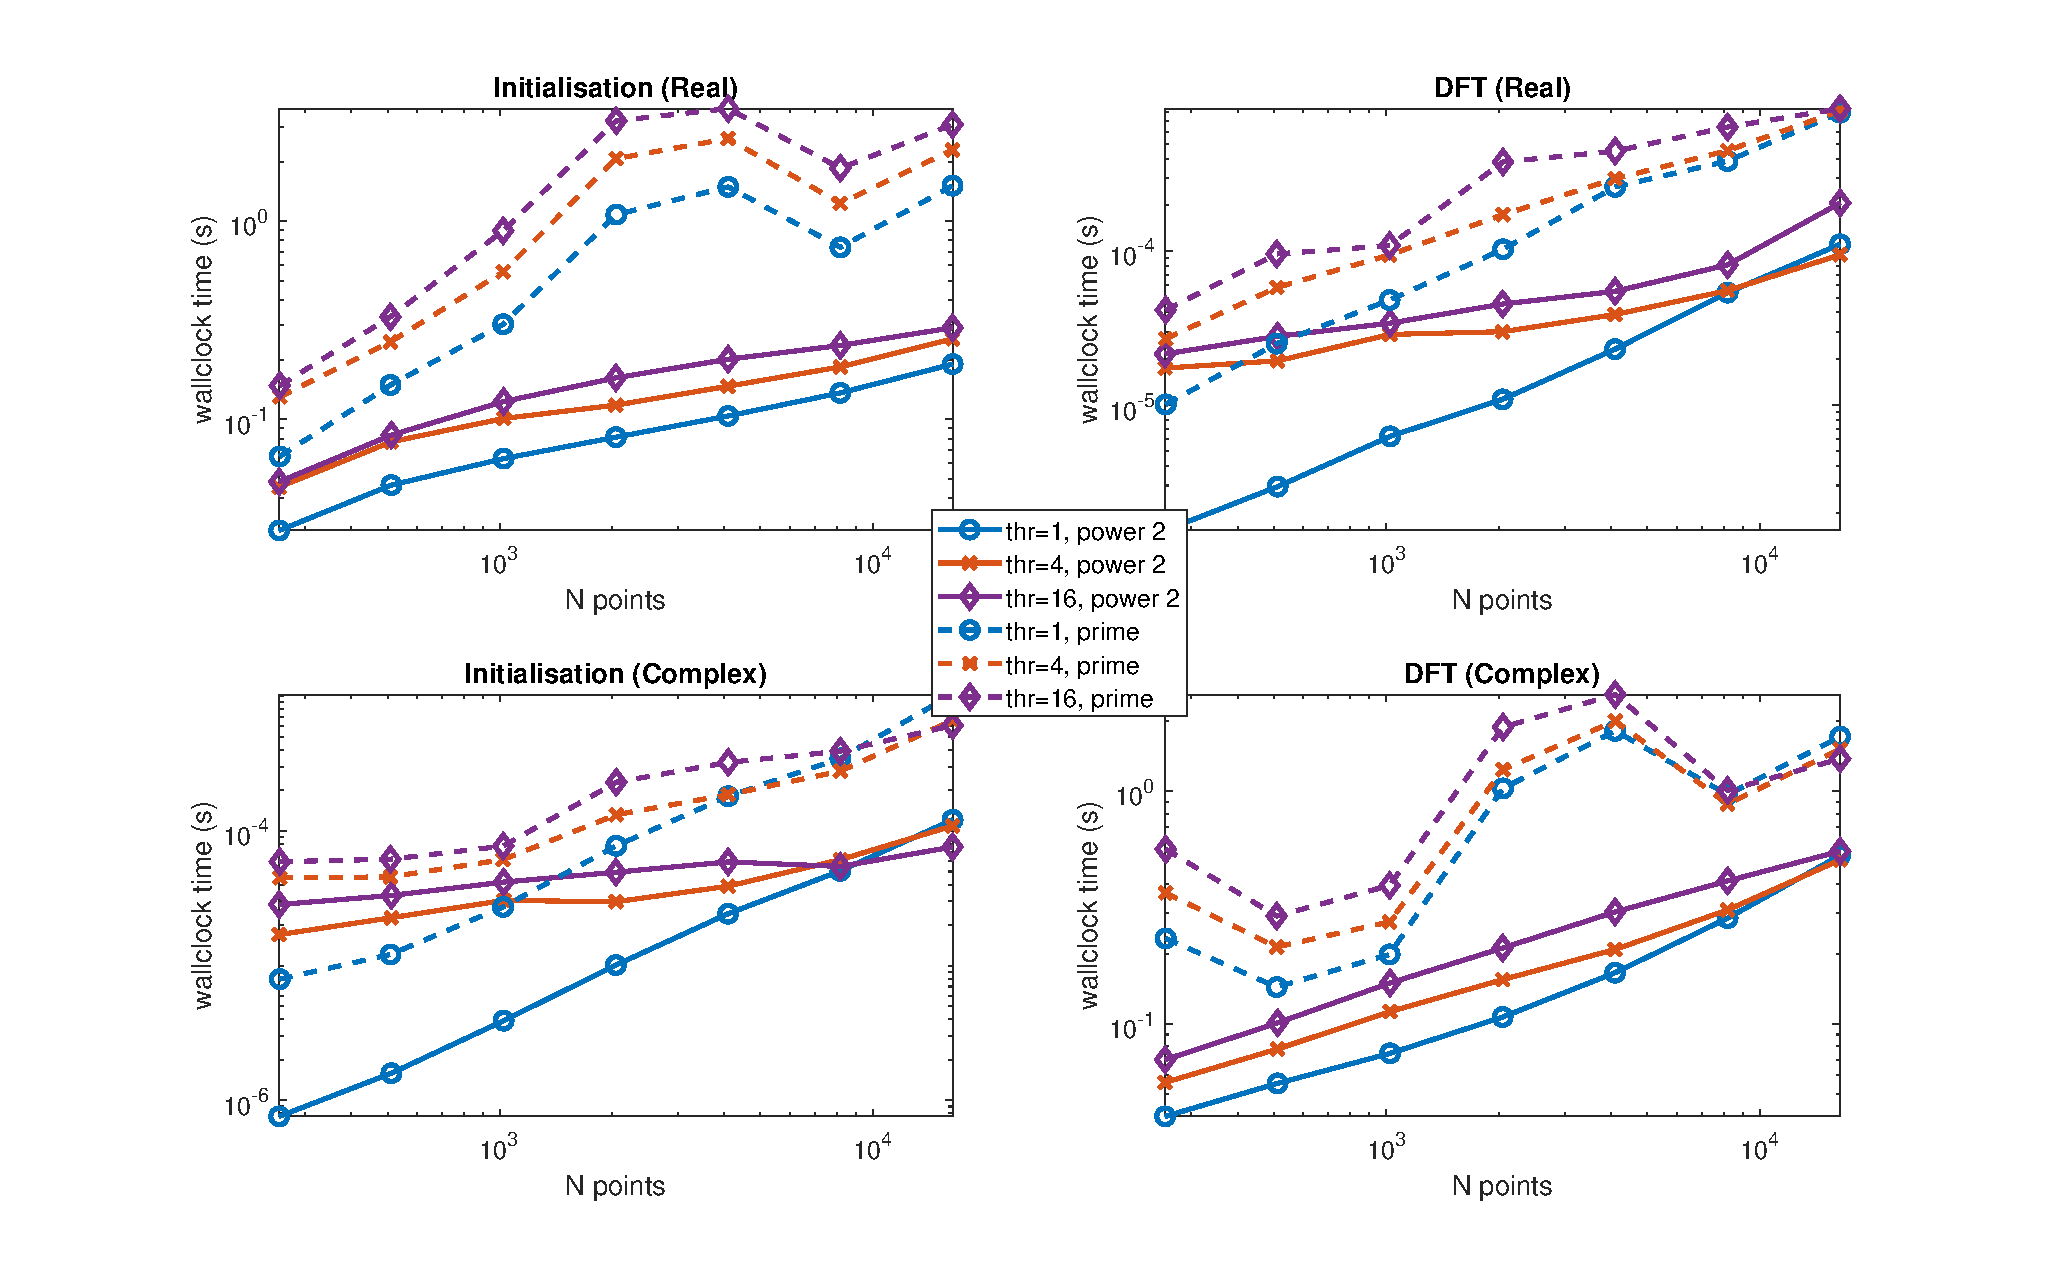
\includegraphics[width=\linewidth]{../results/fftw_1d_thr.eps}
  \caption{Initialisation and DFT execution times of FFTW library applied to 1D signal as a function of the
    number of points, $N,$ and varying the number of threads, $thr.$ }
  \label{1DFFTW}
\end{figure}



\subsection{1D MKL Library}\label{Sec:1DMKL}

The 1D MKL library benchmark runs for 1, 4 and 16 threads ($thr$) are compared
in Figure~\ref{1DMKL}. Initialisation times for $N$ a power of 2 are
nearly always lower than when $N$ is a prime number. For a single
thread, the initialisation time increased as the value of $N$
increased but the rate of increase was much larger when $N$ was
prime. For 4 or 16 threads and $N$ a power of 2, the initialisation
time stays almost constant for $N\le 2^{17}$ and then drops: in the
real case, it then starts rising again for the largest values of $N$
considered. When $N$ is a prime value and 4 or 16 threads are used,
the initialisation times remain almost constant for $N\le 2^{14}$ and
then rises with problem size for larger values of $N.$ For the smaller
values of $N,$ the initialisation times is significantly lower when
one thread is used instead of 4 or 16 (a factor of approximately 10
difference).

As expected, the DFT times are higher when $N$ is prime compared to
$N$ being a power of 2. There is little effect on the DFT time when
the number of threads is varied but $N$ is prime. However, when $N$ is
a power of 2 and greater than $2^{14}$ (real case) or $2^{17}$
(complex case), there is an advantage to using musing multiple threads
with respect to DFT wallclock time. In Table~\ref{Tbl:MKL1d}, we
provide the (wall clock) execution times of the initialisation stage
and the DFT calculations along with their ratio with respect to one
thread for $thr=1,$ 2, 4, 8, 12, 16 and 24. Results for both real and
complex input signals are given for $N=2048,$ 2053, 16381, 16384,
1048573 and 1048576. We observe that when $N$ is prime, there is
little difference between the real and complex results. The DFT time
is almost unchanged when the number of threads is increased but the
initialisation time increases significantly for the two smaller values
of $N$ in the table. Additionally, the initialisation times are
between two and three orders of magnitude larger than the DFT times
for $N=2053$ and 16381. For the largest prime value of $N$ considered,
increasing the number or threads increases the DFT time very slightly
(upto 6\% increase for 24 threads) and also results in a slight
increase in initialisation time (upto 10\%), with the initialisation
time being roughly 90\% greater than the DFT time.

For the values of $N$ that are powers of 2, the table shows that
increasing the number of threads does, in general, result in an
increase in initialisation time and for the smaller values of $N$ the
initialisation time can increase by a factor of almost 10 (real) or 6
(complex): given that there is little difference in DFT time for
differing numbers of threads, we do not advocate using multiple
threads for these smaller values of $N.$ For $N=1048576$ increasing
the number of threads from a single thread results in at most an
increase of 79\% (real) or 32\% (complex) in initialisation time. For
the real case, 16 threads reduces the DFT time by a factor of ~4 and,
for the complex case, the DFT time is reduced by a factor of
~2.4. Given that the initialisation and DFT times are at most a factor
of 10 different, only a small number of DFT computations are required
to overcome the increase in initialisation time.


\begin{figure}[htb]
    \centering
    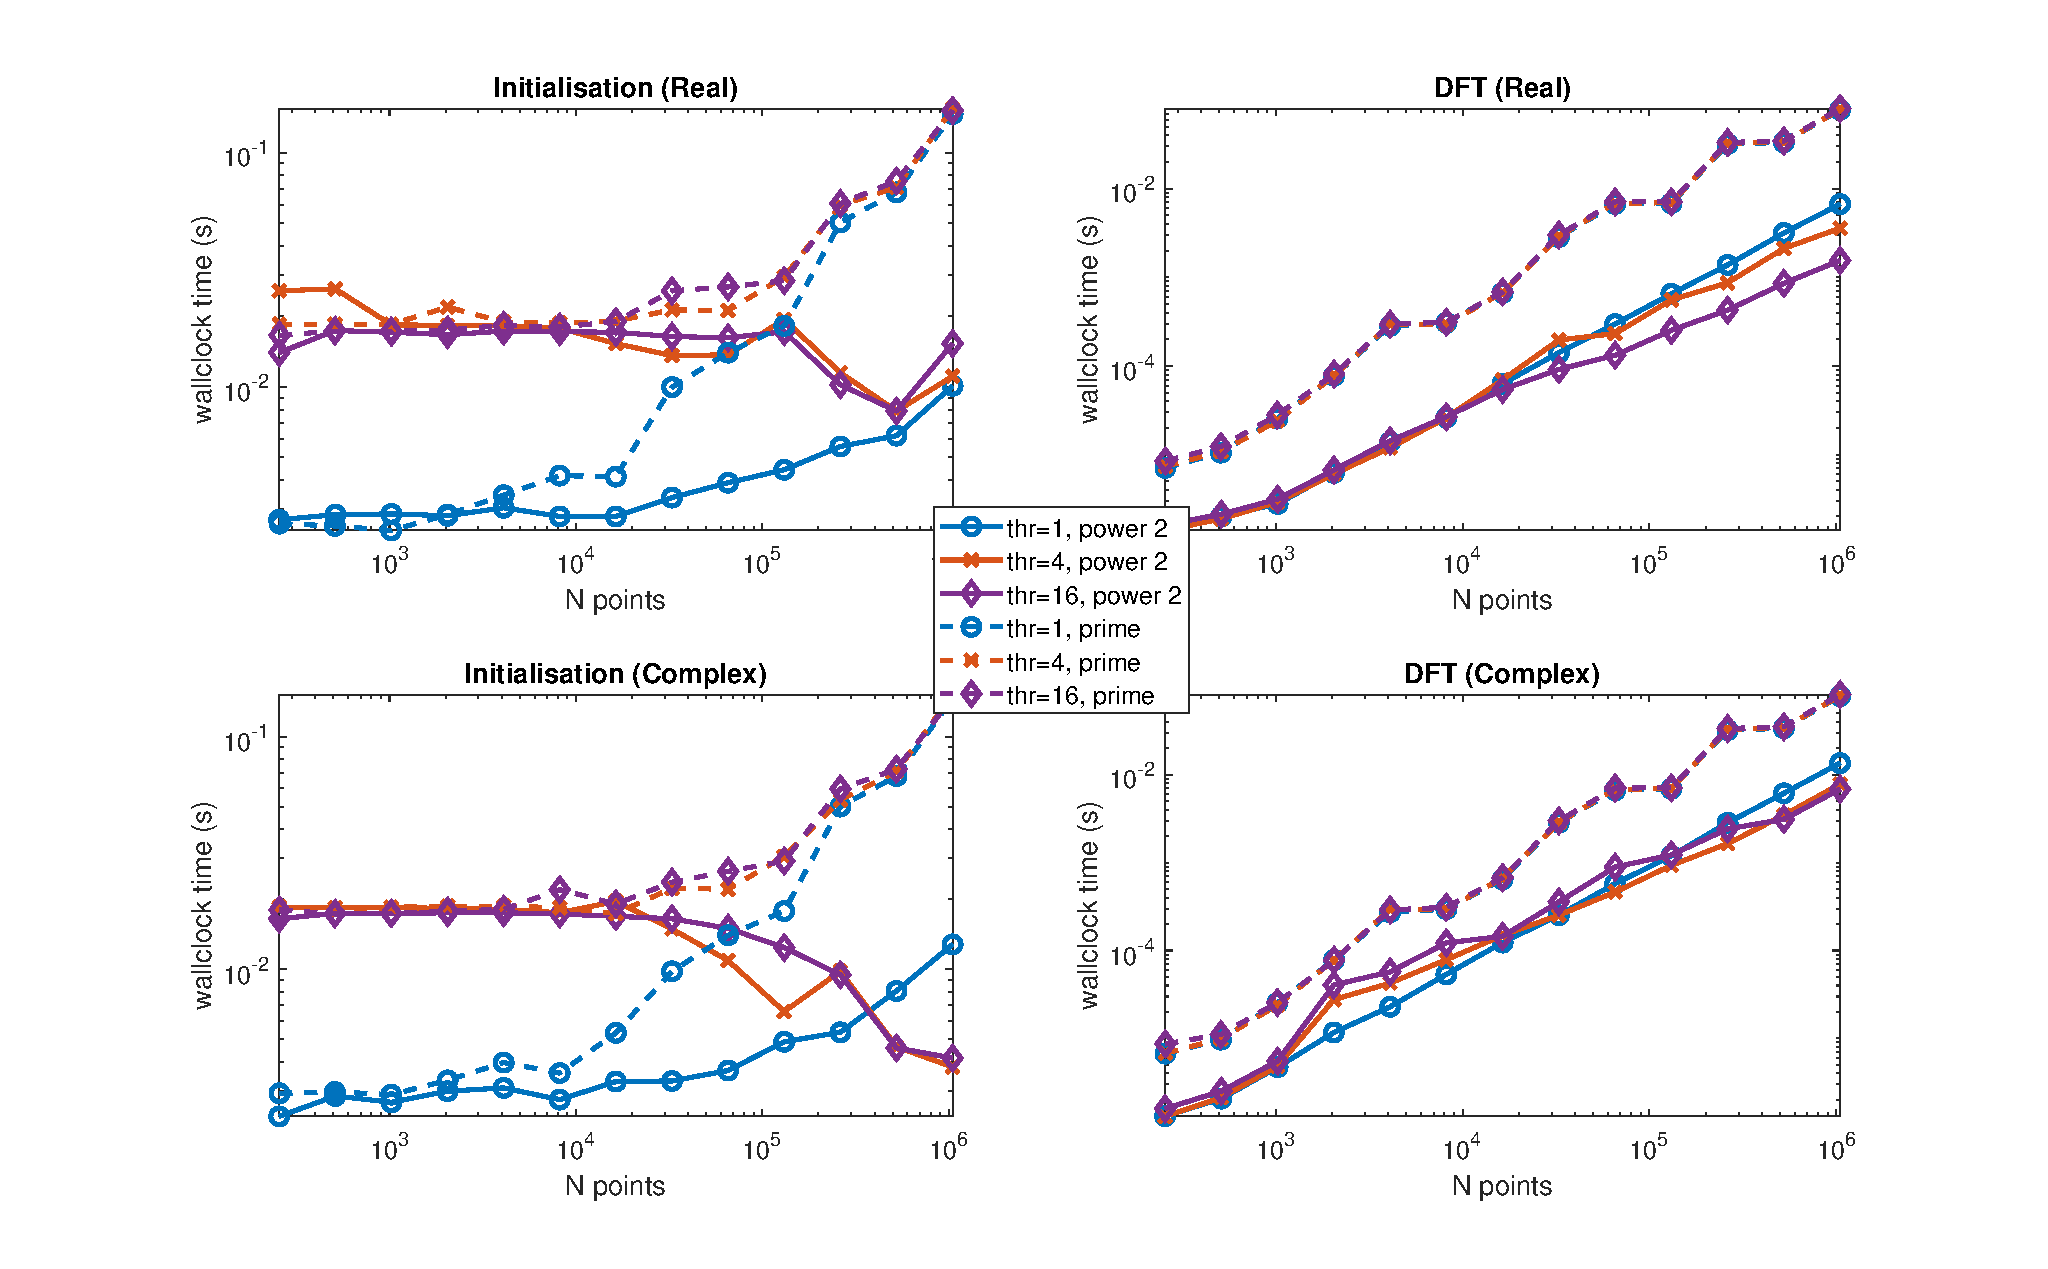
\includegraphics[width=\linewidth]{../results/mkl_1d_thr.eps}
  \caption{Initialisation and DFT execution times of MKL library applied to 1D signal as a function of the
    number of points, $N,$ and varying the number of threads, $thr.$ }
  \label{1DMKL}
\end{figure}






\subsection{Comparison of libraries for 1D benchmarks}\label{Sec:1DComp}

In Figure~\ref{1DFFTWMKL2}, we compare the 1D FFTW and MKL libraries
with multithreading for values of $N$ that are prime numbers. Our
first observation is that, in our computing environment, the MKL
library can perform DFT computations for larger values of $N.$ For the
values of $N$ where we can compare the libraries, MKL has
significantly lower initialisation times. For DFT times, in the real
case, MKL is always faster than FFTW but in the complex case, the MKL
library is best for the very small values of $N$ but as we approach
$N=16384,$ the times appear to be similar. Given the substantial
difference in initialisation time and the larger values of $N$
available for use by the user, we recommend that the MKL library is
used.



\begin{figure}[htb]
    \centering
    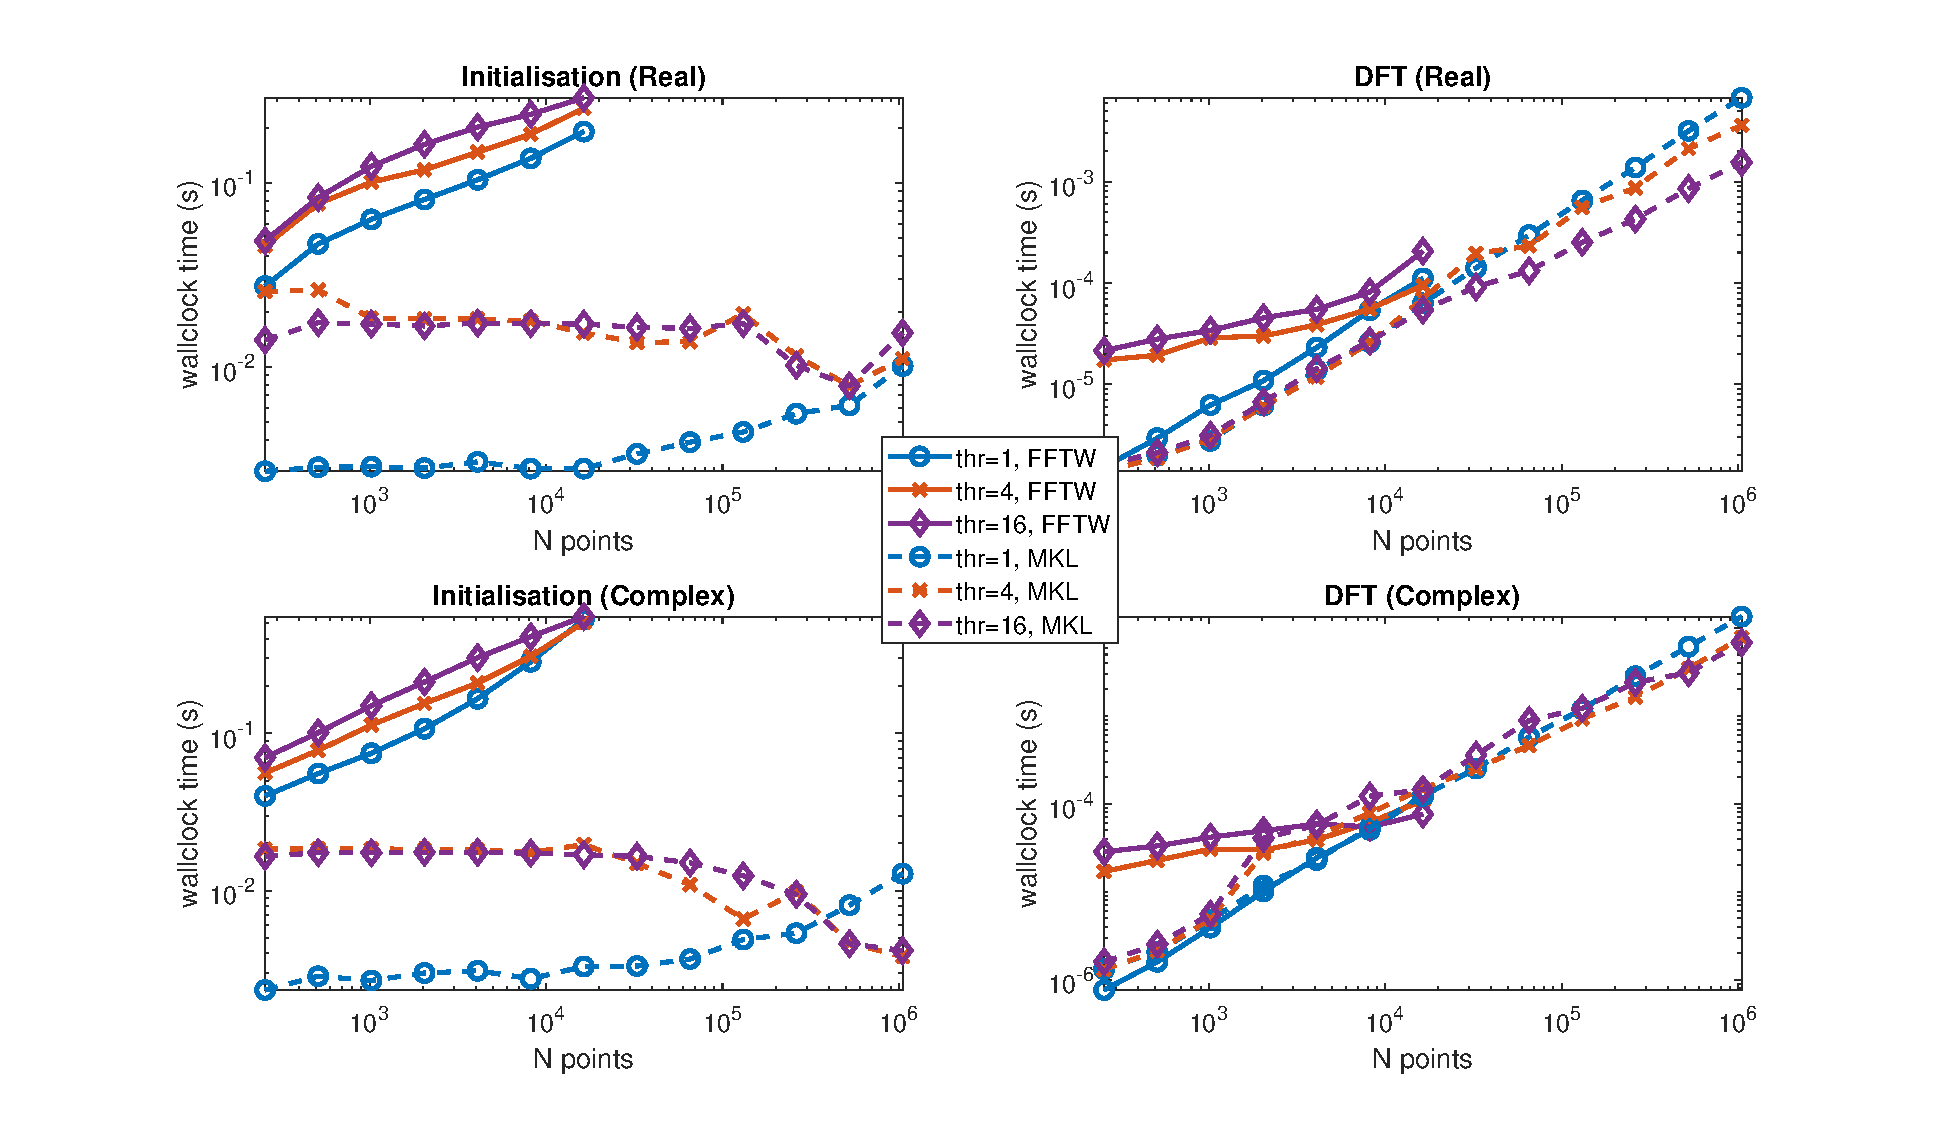
\includegraphics[width=\linewidth]{../results/fftw_mkl_2_1d_thr.eps}
  \caption{Initialisation and DFT execution times of FFTW and MKL libraries applied to 1D signal as a function of the
    number of points, $N,$ and varying the number of threads, $thr.$ $N$ is a power of 2.}
  \label{1DFFTWMKL2}
\end{figure}



The FFTW and MKL libraries are compared in Figure~\ref{1DFFTWMKLPrime}
for prime values of $N.$ As with the case when $N$ is a power of 2,
the initialisation times are significantly lower for the MKL
library. The difference in DFT times is not as pronounced as in the
former case but MKL is still generally faster than FFTW (although, if
the library could accommodate larger values of $N,$ FFTW looks like it
would be faster for these values). Therefore, when $N$ is a prime
number, we recommend using the MKL library over the FFTW library.

\begin{figure}[htb]
    \centering
    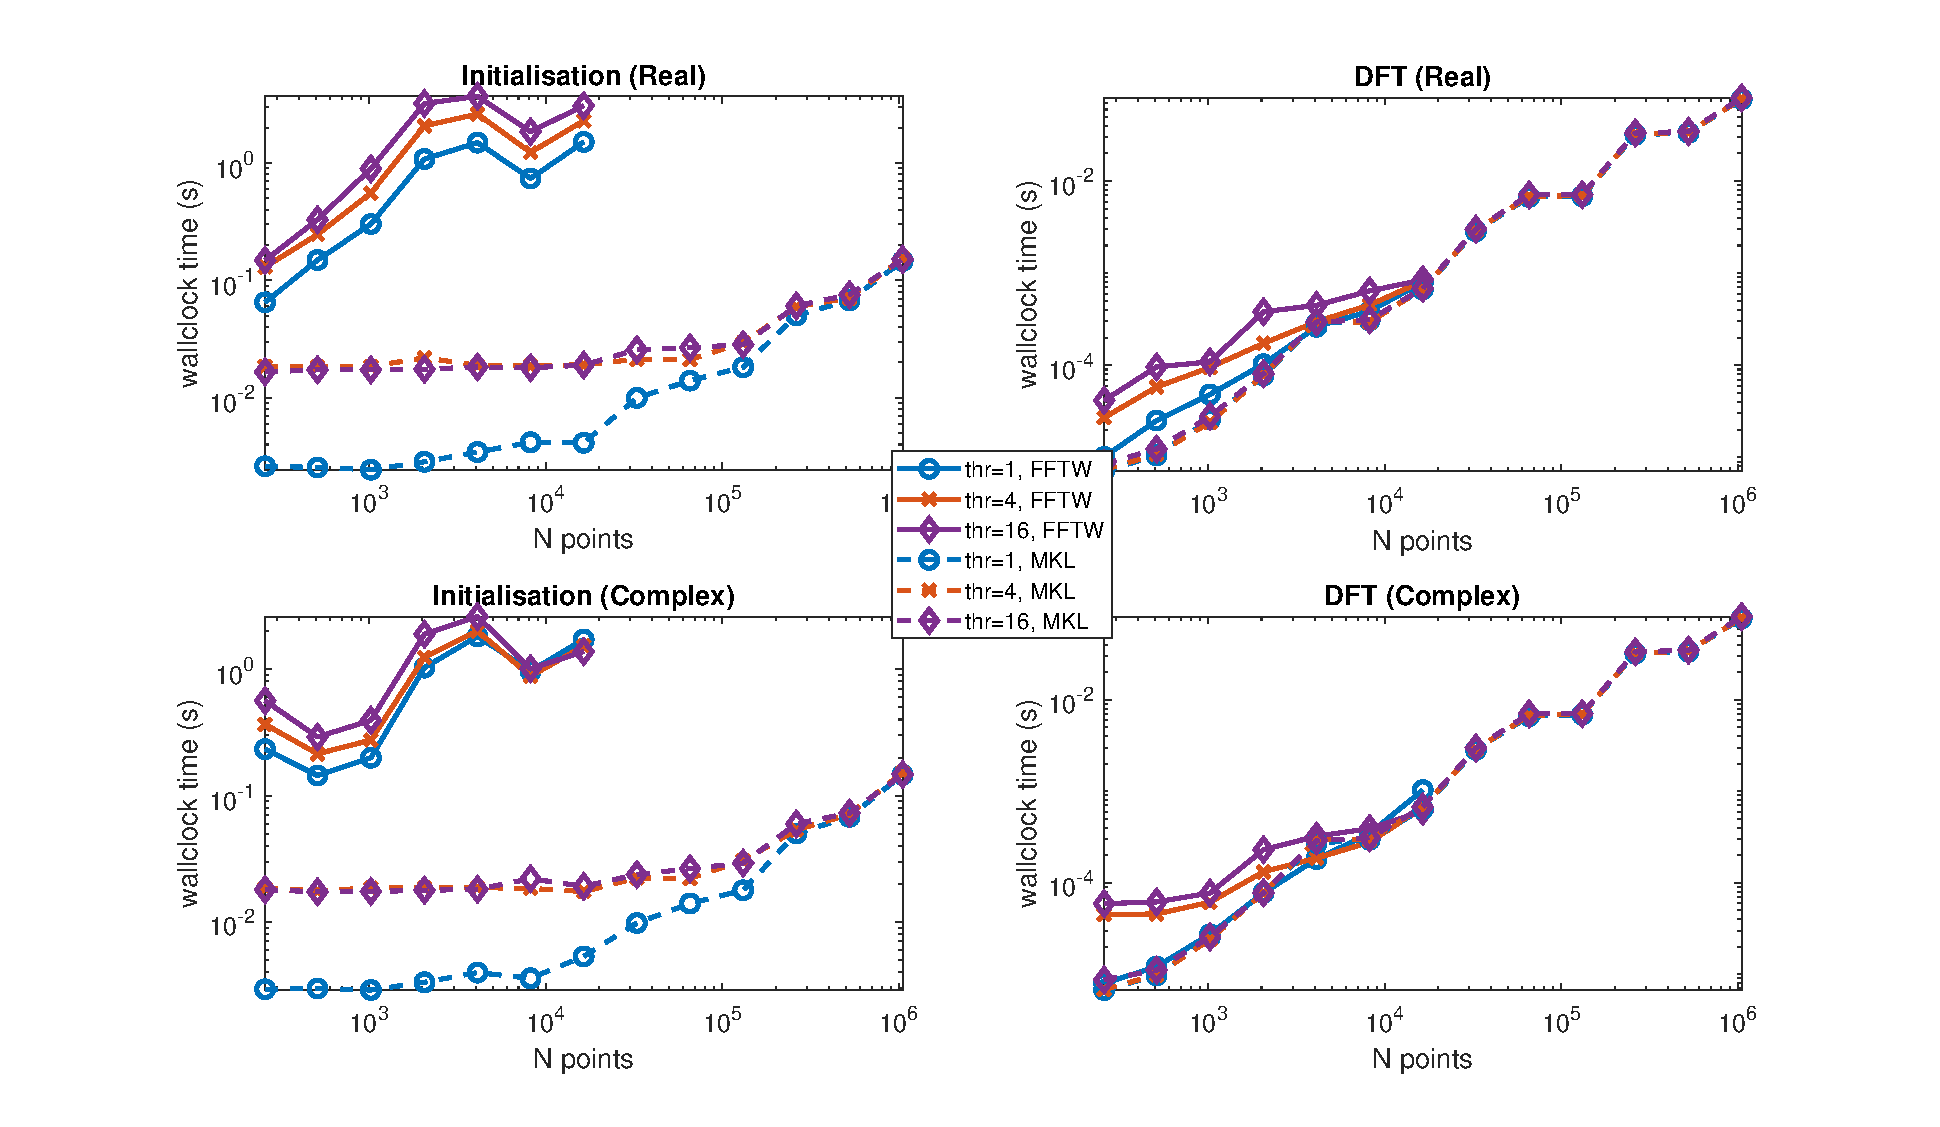
\includegraphics[width=\linewidth]{../results/fftw_mkl_prime_1d_thr.eps}
  \caption{Initialisation and DFT execution times of FFTW and MKL libraries applied to 1D signal as a function of the
    number of points, $N,$ and varying the number of threads, $thr.$ $N$ is a prime number.}
  \label{1DFFTWMKLPrime}
\end{figure}


\section{Effect of domain size and multithreading for 2D benchmarks}\label{Sec:2DMulti}
The benchmark results for libraries that perfrom the fast Fourier
transform over a 2D domain are discussed in this section. As with the
1D results in Section~\ref{Sec:1DMulti}, the P3DFFT library cannot be
used on these problems so we compare the OpenMP versions of the FFTW
and MKL libraries.

Similarly to the benchmarks in Section~\ref{Sec:1DMulti}, we set
$n_3=4,$ $n_q=4$ and $n_1=n_2=N,$ were $N$ is defined as follows.  For one
set of tests, we let $N=2^k$ for $k=5,\ldots,12.$ For the other set of
tests, $N$ is defined to be the closest prime number to $2^k,$
$k=5,\ldots,12:$ if two primes are equidistant, we choose the larger
one.

\subsection{2D FFTW Library}\label{Sec:2DFFTW}

In Figure~\ref{2DFFTW}, we compare our single node benchmark
experiments for the multithreaded FFTW library for 1, 4 and 16 OpenMP
threads. There is a difference in behaviour between the real and
complex benchmarks. For $N$ smaller than 200, the initialisation times
for the real case are smaller when $N$ is prime compared to when $N$
is a power of 2; for the complex case, the initialisation times for
$N$ prime are, in general, greater than $N$ a power of 2. For larger
values of $N,$ the initialisation times for prime values of $N$ are
larger than $N$ a power of 2 in both the real and complex cases but
the complex initialisation times appear to be higher than in the real
case. Increasing the number of threads also increases the
initialisation times but, as the problem size increases, the
difference between 4 and 16 threads generally diminishes. For further
clarity of the benchmark results, we provide the (wall clock)
execution times of the initialisation stage and the DFT calculations
along with their ratio with respect to one thread for $thr=1,$ 2, 4,
8, 12, 16 and 24 in Table~\ref{Tbl:FFTW2d}. Results for both real and
complex input signals are given for $N=31,$ 32, 256, 257, 2048 and
2053. These confirm that the initialisation times are lower for the
real case compared to the complex case. Additionally, increasing the
number of threads has less of an effect when $N$ is prime compared to
when $N$ is a power of 2. However,

Comparing the DFT times in Figure~\ref{2DFFTW}, for the larger values
of $N,$ increasing the number of threads is always improving the
wallclock time. When $N$ is a power of 2, a single thread is
prefereable for $N\le 128.$ The DFT times are larger when $N$ is a
prime number instead of being a power of 2. Using
Table~\ref{Tbl:FFTW2d}, we see observe that increasing the number of
threads results in lower ratios when $N$ is a prime compared to when
$N$ is a power of 2. Given that the initialisation times are at least
one order of magnitude larger than the DFT times, when a small number
of DFT calculations are being performed with a single initialisation,
it is normally best to use a single thread when $N$ is small (less
than 300) but for a large value of $N$ we recommend using 16 or 24
threads (the latter if performing a large number of DFT calculations).




\begin{figure}[htb]
    \centering
    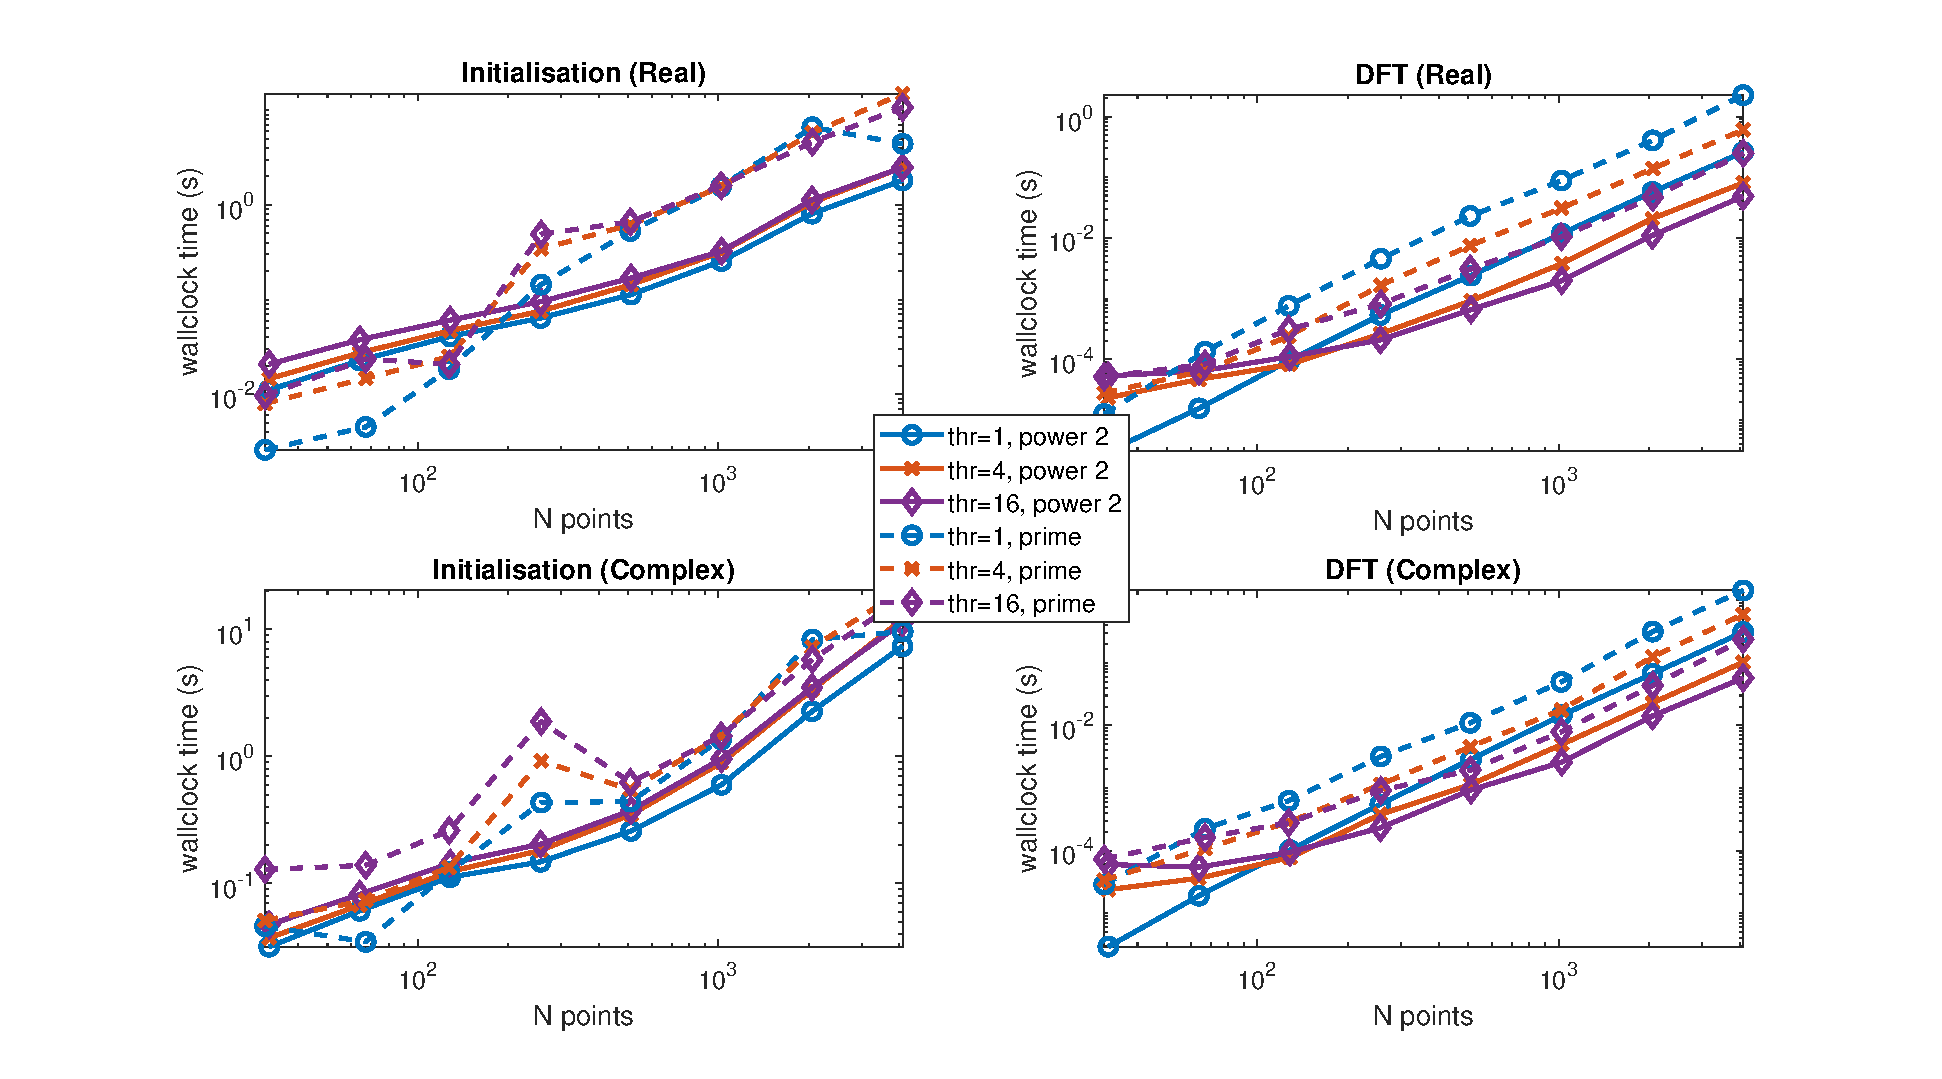
\includegraphics[width=\linewidth]{../results/fftw_2d_thr.eps}
  \caption{Initialisation and DFT execution times of FFTW library applied to 2D signal as a function of the
    number of points, $N,$ and varying the number of threads, $thr.$ }
  \label{2DFFTW}
\end{figure}



\subsection{2D MKL Library}\label{Sec:2DMKL}

In Figure~\ref{2DMKL} we do the same comparisions as in
Figure~\ref{2DFFTW} but for the MKL library. For a single thread, when
$N$ is lower than 600, the initialisation times remain roughly
constant as $N$ increases and, once $N$ is greater than 600, the
initialisation time increases but at a faster rate for real signal
inputs. When mulitple threads are used, the initialisation time is
initially high but starts to decrease as $N$ increases. For 16
threads, this decrease starts sooner when the input signal is complex
and, once $N$ is greater than 1000, the multiple threads leads to
smaller initialisation times than when a signal thread is used; in the
real case, the multithreads have improved initialisation times for
$N>2000.$ In general, there is little difference between $N$ being
prime and a power of 2 for one or 16 threads with real input signals
although, for the larger values of $N$, the initialisation time is
better when $N$ is a power of 2. For complex input signals, switching
between $N$ being a power of two and $N$ being prime has little effect
on the initialisation time when one or four threads is used. For the
larger problem sizes, increasing the number of threads has a positive
affect on the initialisation time.  This is confirmed in
Table~\ref{Tbl:MKL2d}, where we see that the initialisation time is
roughly halved when 24 threads are used compared to a single thread.



\begin{figure}[htb]
    \centering
    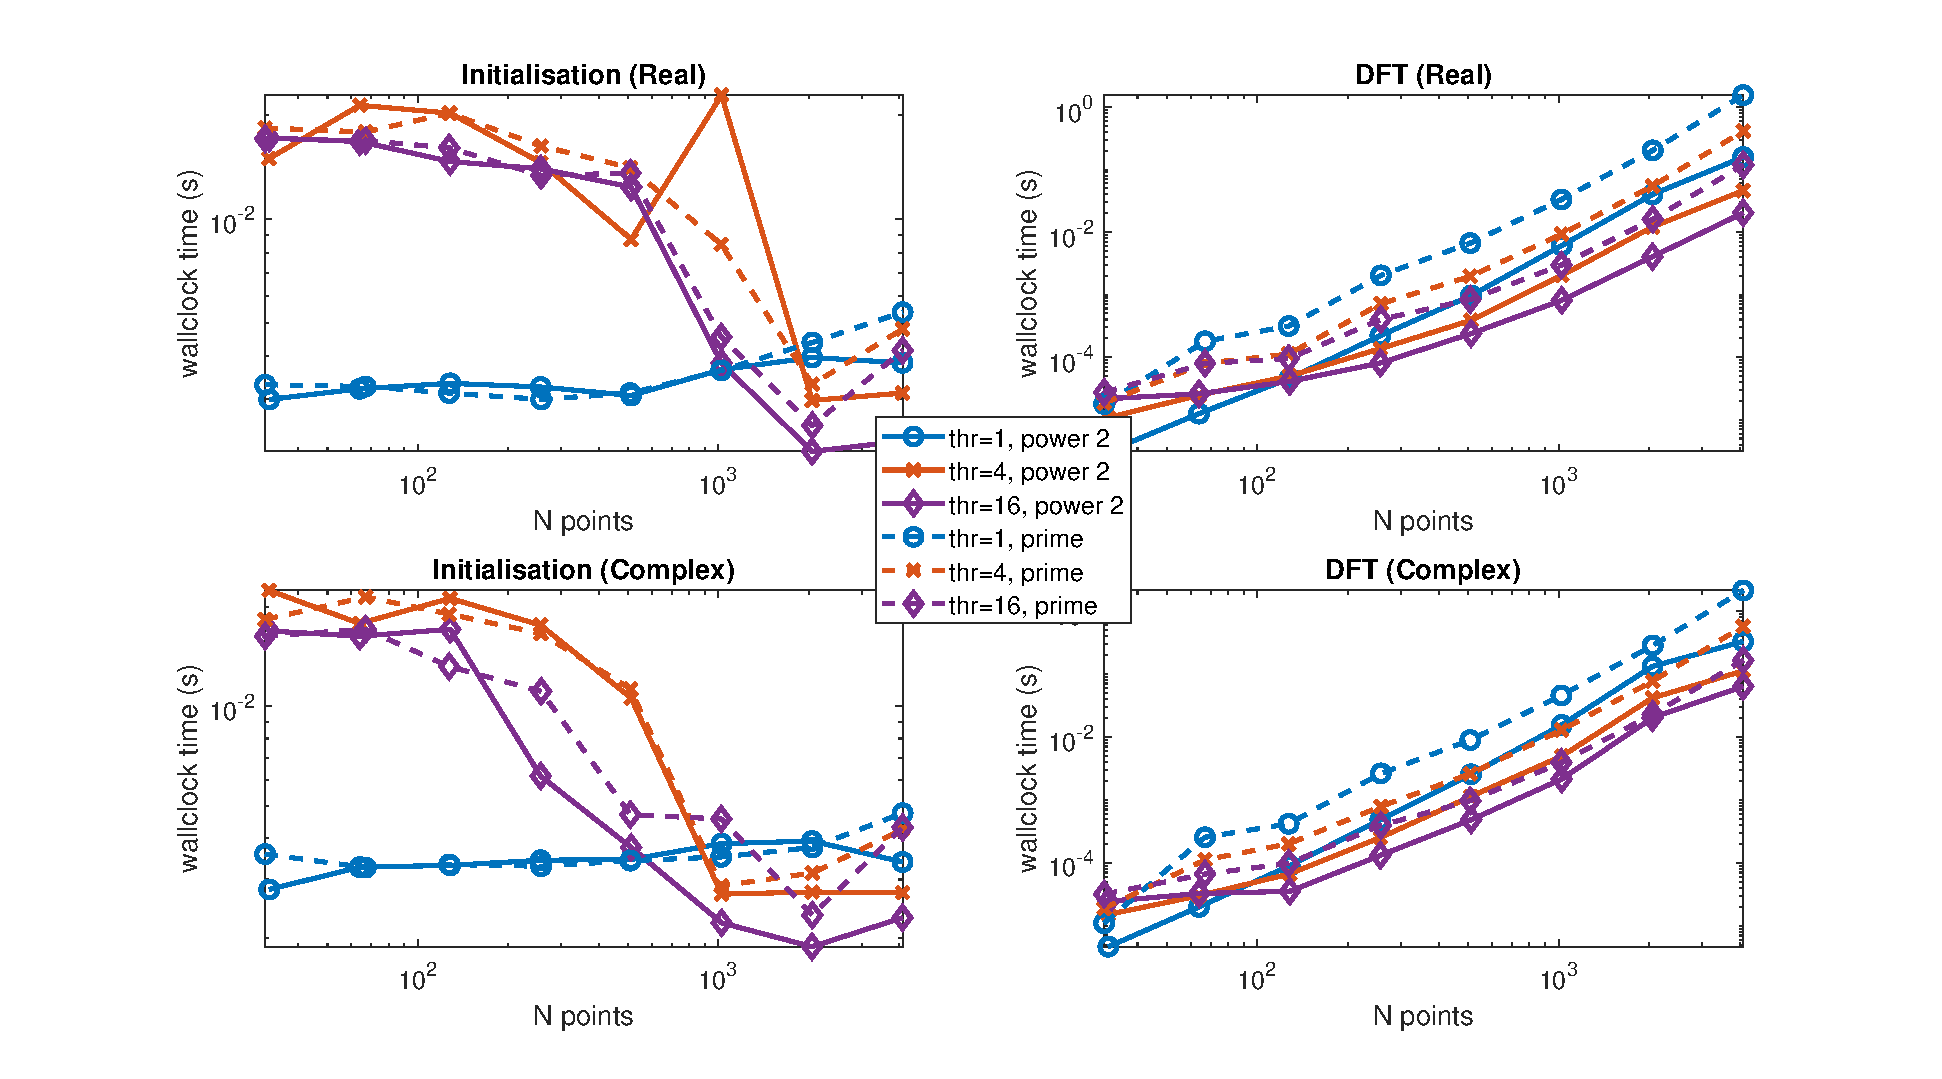
\includegraphics[width=\linewidth]{../results/mkl_2d_thr.eps}
  \caption{Initialisation and DFT execution times of MKL library applied to 2D signal as a function of the
    number of points, $N,$ and varying the number of threads, $thr.$ }
  \label{2DMKL}
\end{figure}




As expected, in Figure~\ref{2DMKL} we observe that increasing the
problem size increases the DFT calculation time. Except for the very
smallest value of $N,$ where $N$ is prime, increasing the number of
threads from 1 to 4 to 16 produces monotonic reductions in the DFT
time in both the real and complex cases. For $N$ a power of 2 and
smaller than 256 (real case) or 128 (complex case), using multiple
threads increases the DFT time. For larger values of $N,$ multiple
threads decreases the DFT times. This is confirmed in
Table~\ref{Tbl:MKL2d} but we see that there is little gain with
respect to DFT time in going above 12 threads. However, the additional
reduction in initialisation time for using more than 12 threads for
large values of $N$ leads us to conclude that, on a single node of
ARCHER, it is advantageous to use all the threads available when $N$
is greater than 2000 (real case or complex case with $N$ prime) or
1000 (complex case with $N$ a power of 3). For $N=256,$ we can work
out the number of DFT calculations, $k,$ that would be required for
$thr$ threads to have a lower time than a single thread when
performing a single initialisation and $k$ DFT calculations. We
provide this information in Table~\ref{Tbl:MKL2dk} and observe that
multithreading can be positively utilised for lower values of $k$ when
$N$ was prime because of the greater time to perform a DFT calculation
(a factor of 4-5 difference) but the initialisation times are, in
general, similar. Additionally, the complex case also requires smaller
values of $k$ compared to the real case.



\begin{table}
\begin{center}
%\being{small}
\begin{tabular}{|r||r|r||r|r|}
  \hline
 & \multicolumn{2}{|c||}{$k(N=256)$} & \multicolumn{2}{|c|}{$k(N=257)$} \\
$thr$ &  Real & Complex &  Real & Complex  \\ \hline
  2 & 49 & 0   &  1 & 2 \\
  4 & 135 & 62 & 11 & 8 \\
  8 & 70 & 42 & 12 & 8 \\
  12 & 86 & 29 & 11 & 3 \\
  16 & 77 & 8  & 7 & 4 \\
  24 & 83 & 31 &10 & 6  \\ \hline
\end{tabular}
\caption{ For $N=256$ and $N=257,$ the number of DFT calculations, $k,$ required for $thr$ threads to have a lower wallclock time than a single thread when performing  a single initialisation and $k$ DFT calculations are performed with the 2D interface to the FFTW library.  }\label{Tbl:MKL2dk}
%\end{small}
\end{center}
\end{table}

\subsection{Comparison of libraries for 2D benchmarks}\label{Sec:2DComp}

In Figure~\ref{2DFFTWMKL2}, we compare the initialisation and DFT
wallclock times for the FFTW and MKL libraries with our 2D benchmark
runs for $N$ a power of 2. For the real case, there is a stark
difference in initialisation times as $N$ grows with MKL being faster:
when $N=4096$ the FFTW time is a factor of 475 larger than that of MKL
when a single thread is used; for $thr=4,$ the factor is 800; and for
$thr=24,$ factor is 1500. Looking at Figure~\ref{2DFFTWMKL2}, the
complex case appears to have similar differences in initialisation
times but for $N=4096,$ the factors are 2170, 4380 and 3350 for
$thr=1,$ 4 and 24, respectively. Additionally, the MKL DFT wallclock
times are lower than those of FFTW (real case) or, in general, very
similar for the complex case. Thus, when $N$ is a power of 2, we
recommend using the MKL library.


\begin{figure}[htb]
    \centering
    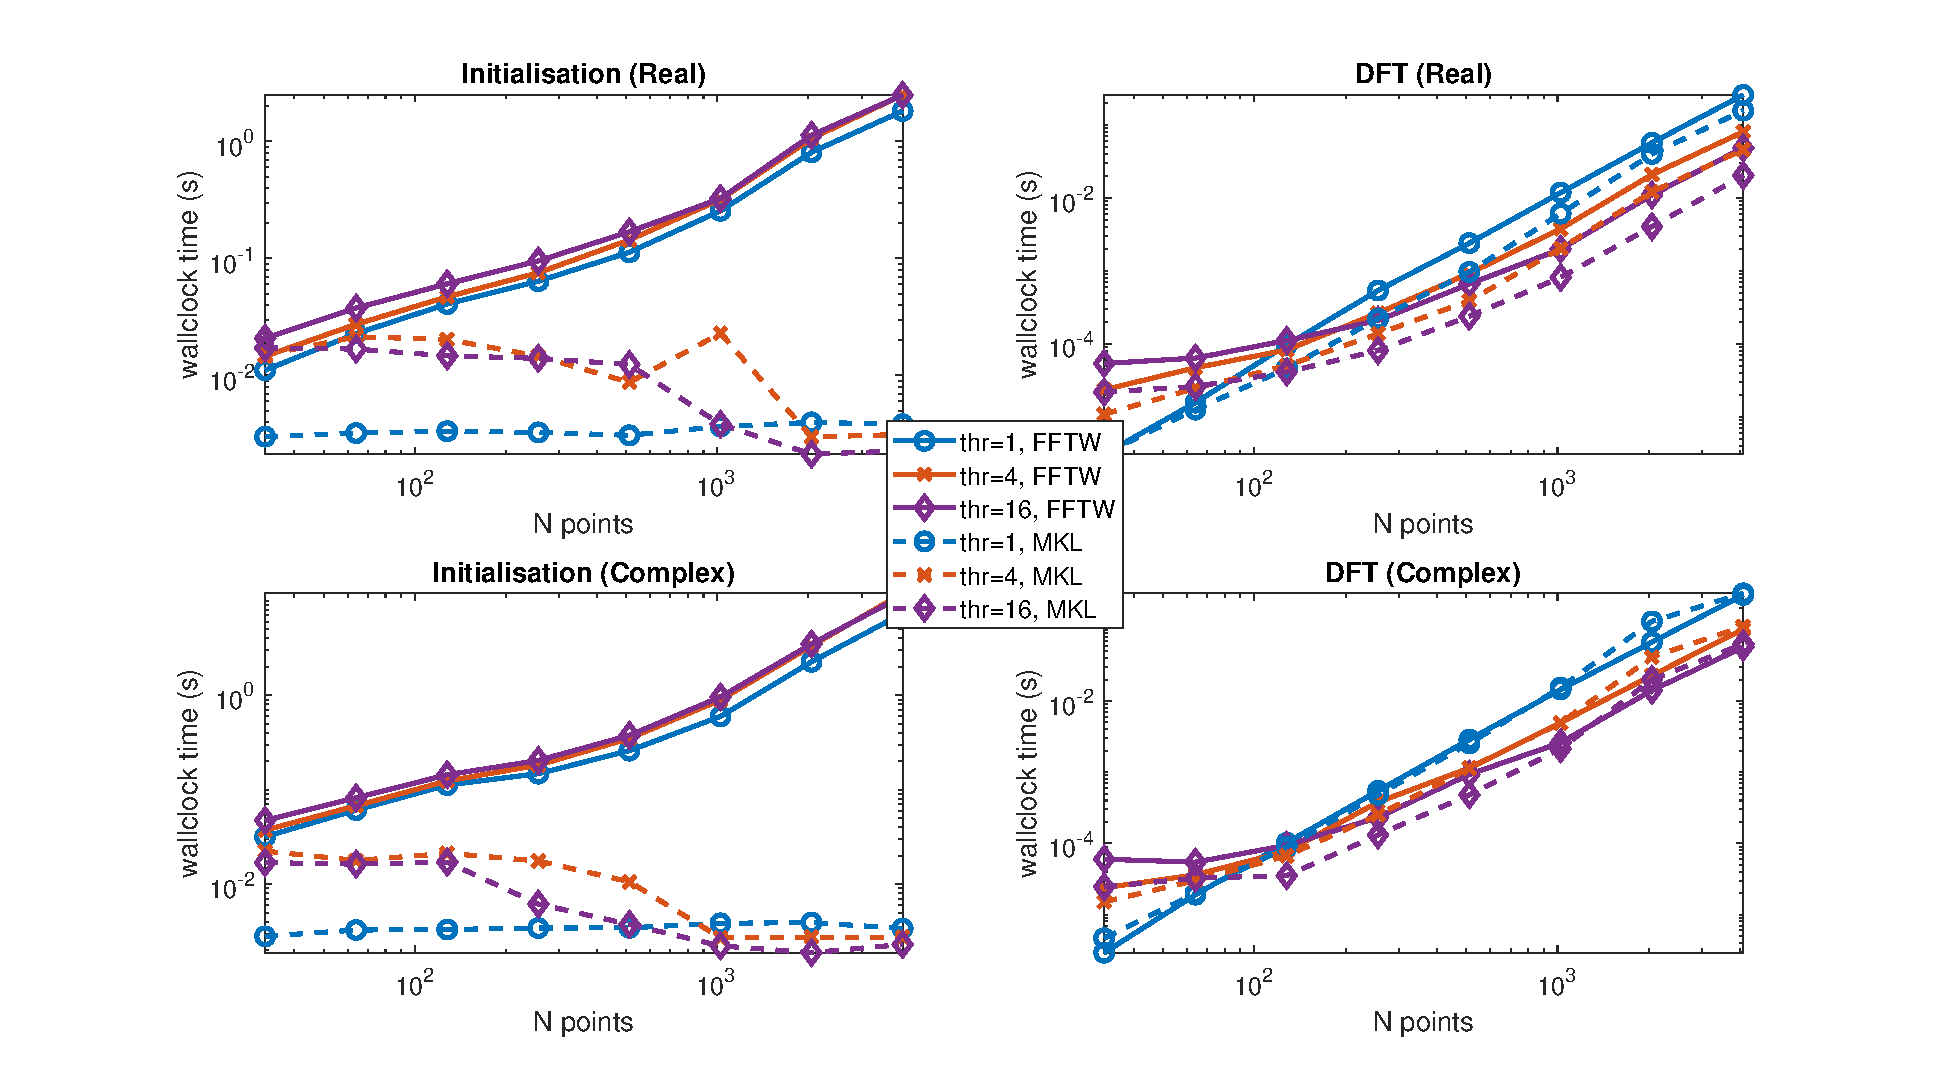
\includegraphics[width=\linewidth]{../results/fftw_mkl_2_2d_thr.eps}
  \caption{Initialisation and DFT execution times of FFTW and MKL libraries applied to 2D signal as a function of the
    number of points, $N,$ and varying the number of threads, $thr.$ $N$ is a power of 2.}
  \label{2DFFTWMKL2}
\end{figure}


We compare the FFTW and MKL library initialisation and DFT times for
prime values of $N$ in Figure~\ref{2DFFTWMKLPrime}. As with the case
when $N$ is a power of 2, there is a marked difference in
initialisation time for large values of $N$ with the MKL library have
significantly lower times. For $N=4099$ with $thr=1,$ 4 and 24, the
difference in initialisation time is a factor of 820, 3120 and 1920,
respectively, for the real case, and 2010, 4750 and 5360,
respectively. In general, the DFT times are slightly better for the
MKL library in both the real and complex cases and, hence, we
recommend using the MKL library.

\begin{figure}[htb]
    \centering
    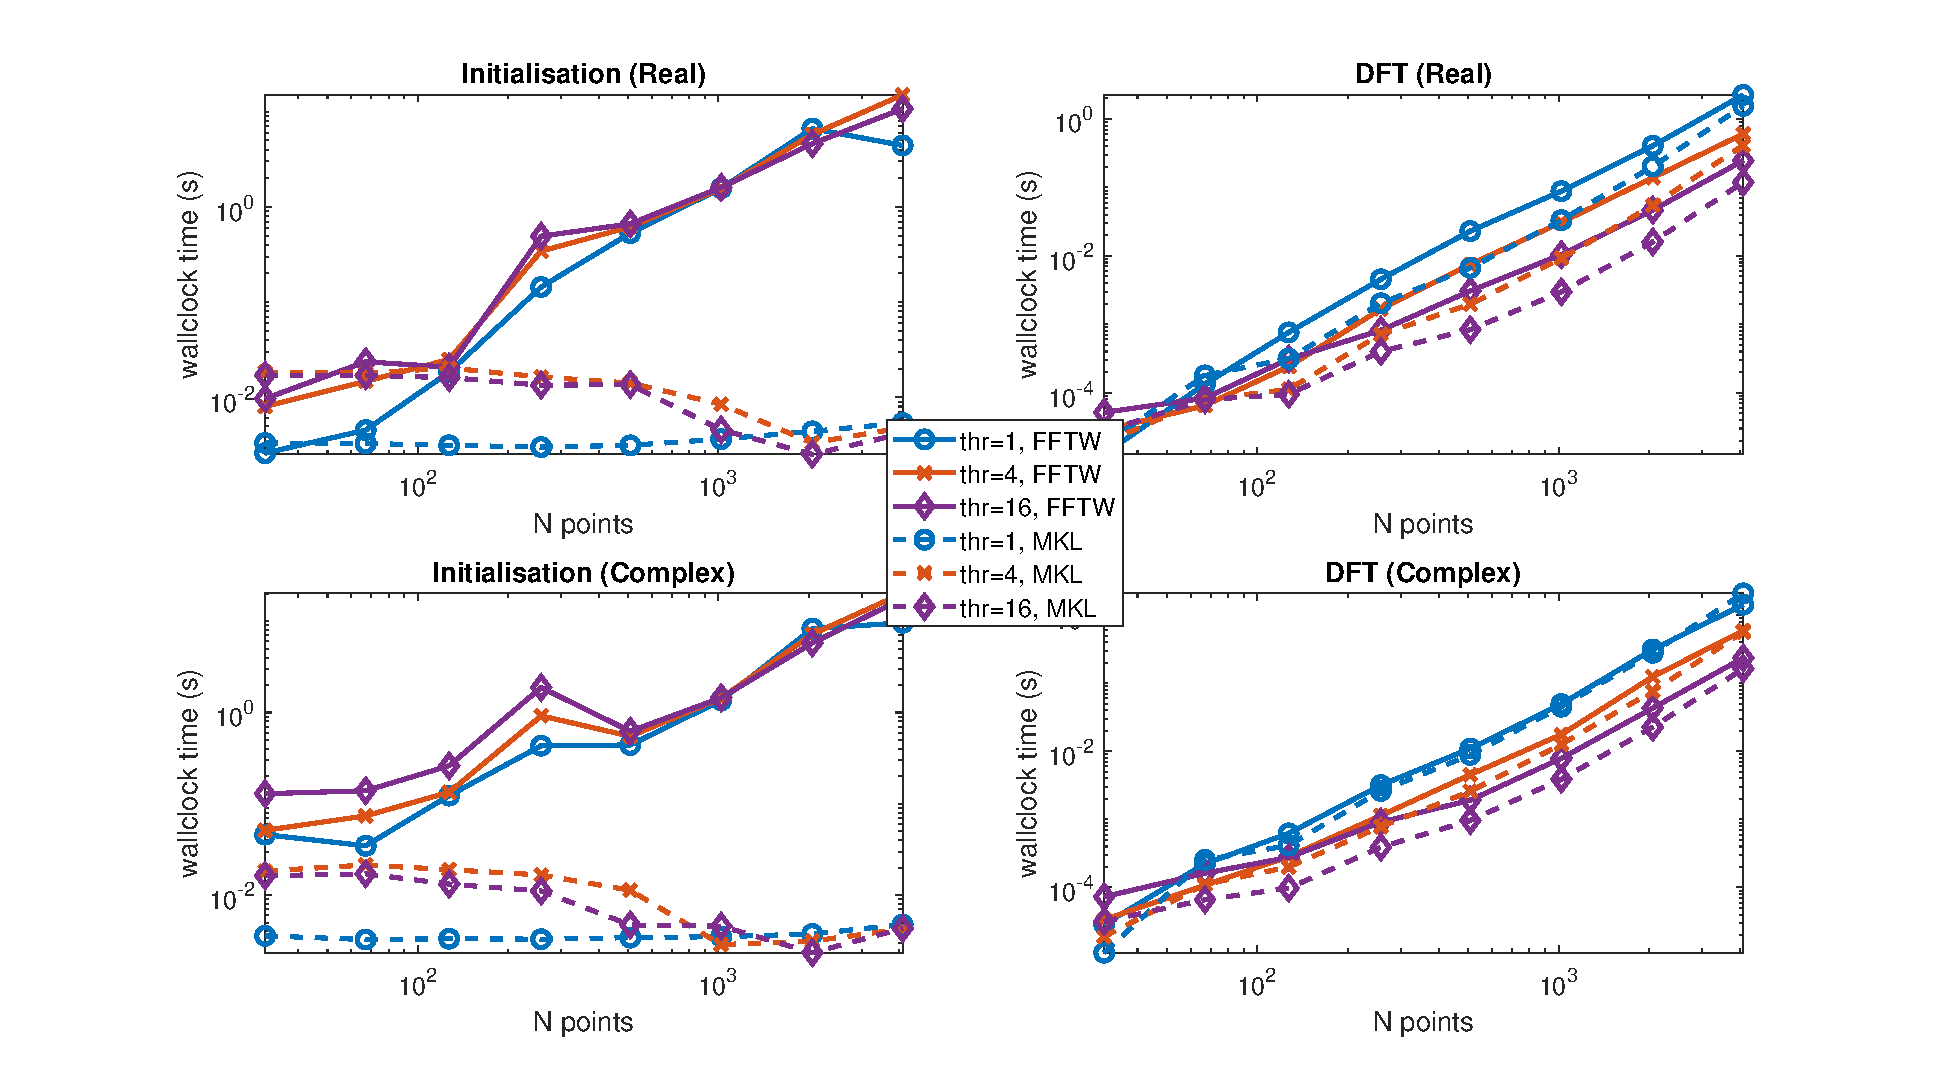
\includegraphics[width=\linewidth]{../results/fftw_mkl_prime_2d_thr.eps}
  \caption{Initialisation and DFT execution times of FFTW and MKL libraries applied to 2D signal as a function of the
    number of points, $N,$ and varying the number of threads, $thr.$ $N$ is a prime number.}
  \label{2DFFTWMKLPrime}
\end{figure}





\section{Effect of domain size and multithreading for 3D benchmarks}\label{Sec:3DMulti}
The results for libraries that perform the fast Fourier transform over
a 3D domain are discussed in this section. The P3DFFT library only
provides a version with both MPI and OpenMP provision and, hence, we
use this version of the library but set the number of MPI processes to
one.

Similarly to the benchmarks in Section~\ref{Sec:1DMulti} and \ref{Sec:2DMulti}, we set
$n_q=4$ and $n_1=n_2=n_3=N,$ were $N$ is defined as follows.  For one
set of tests, we let $N=2^k$ for $k=3,\ldots,9.$ For the other set of
tests, $N$ is defined to be the closest prime number to $2^k,$
$k=3,\ldots,9:$ if two primes are equidistant, we choose the larger
one.

\subsection{3D FFTW Library}\label{Sec:3DFFTW}
The initialisation and DFT times for the FFTW library applied to the
3D benchmark are compared in Figure~\ref{3DFFTW} for 1, 4 and 16
threads. Initialisation times for a single thread are generally lower
than when 4 or 16 threads are used and, in general, the initialisation
times are slightly higher for prime values of $N$ compared to when
they are a power 2. In both the real and complex cases, when $N$ is a
power of 2, it is better to use a single thread with respect to DFT
calculation time for $N$ smaller than 32 and, when $N$ is larger than
32, we start to see the gains in using multiple threads. When $N$ is
prime, multithreading becomes advantageous for values of $N$ greater
than 31 with respect to DFT times. 

To further analyse the benchmark results, we provide the DFT and
initialisation wall clock times for $N=7,$ 8, 31, 32, 509 and 512 with
1,2,4,8,16 and 24 threads. When $N=7$ or 8, the use of multiple
threads has a catastrophic affect on the DFT time: 24 threads results
in a factor of 62 (real case) or 75 (complex case) increase in DFT
time when $N=7$ and a factor 47 (real case) or 82 (complex case) when
$N=8;$ additionally, the initialisation times triple in the complex
case and increase by a factor of 5 for the real case. When $N=31,$
increasing the number of threads results in the DFT wallclock time
decreasing but the initialisation time increases: in
Table~\ref{Tbl:FFTW3dk} we provide the number of DFT calculations,
$k,$ (on average) that would be required for $thr$ threads to have a
lower time than a single thread when performing a single
initialisation and $k$ DFT calculations for $N=31,$ 32, 509 and
$N=512.$ For $N=31,$ (on average) increasing the number of threads is
never going to improve the overall time spent initialising and then
performing a DFT when the input is complex. However, for real input,
83 or more DFTs per initialisation will see an improvement in wall
clock when using 8 threads over using a single thread. For $N=32,$
hundreds of DFTS per initialisation are required in the cases where it
is possible to outperform a single thread. With real signals and
$N=509,$ it is always advantageous to use multithreading with the
architecture and benchmark set-up that we used, and 24 threads is
optimal on a single node with respect to wallclock time. For complex
input signals with $N=509,$ when 8 or more threads are used, just 2 or
more DFT calculations per initialisation will see a saving in overall
wallclock time over using a single thread.

\begin{figure}[htb]
    \centering
    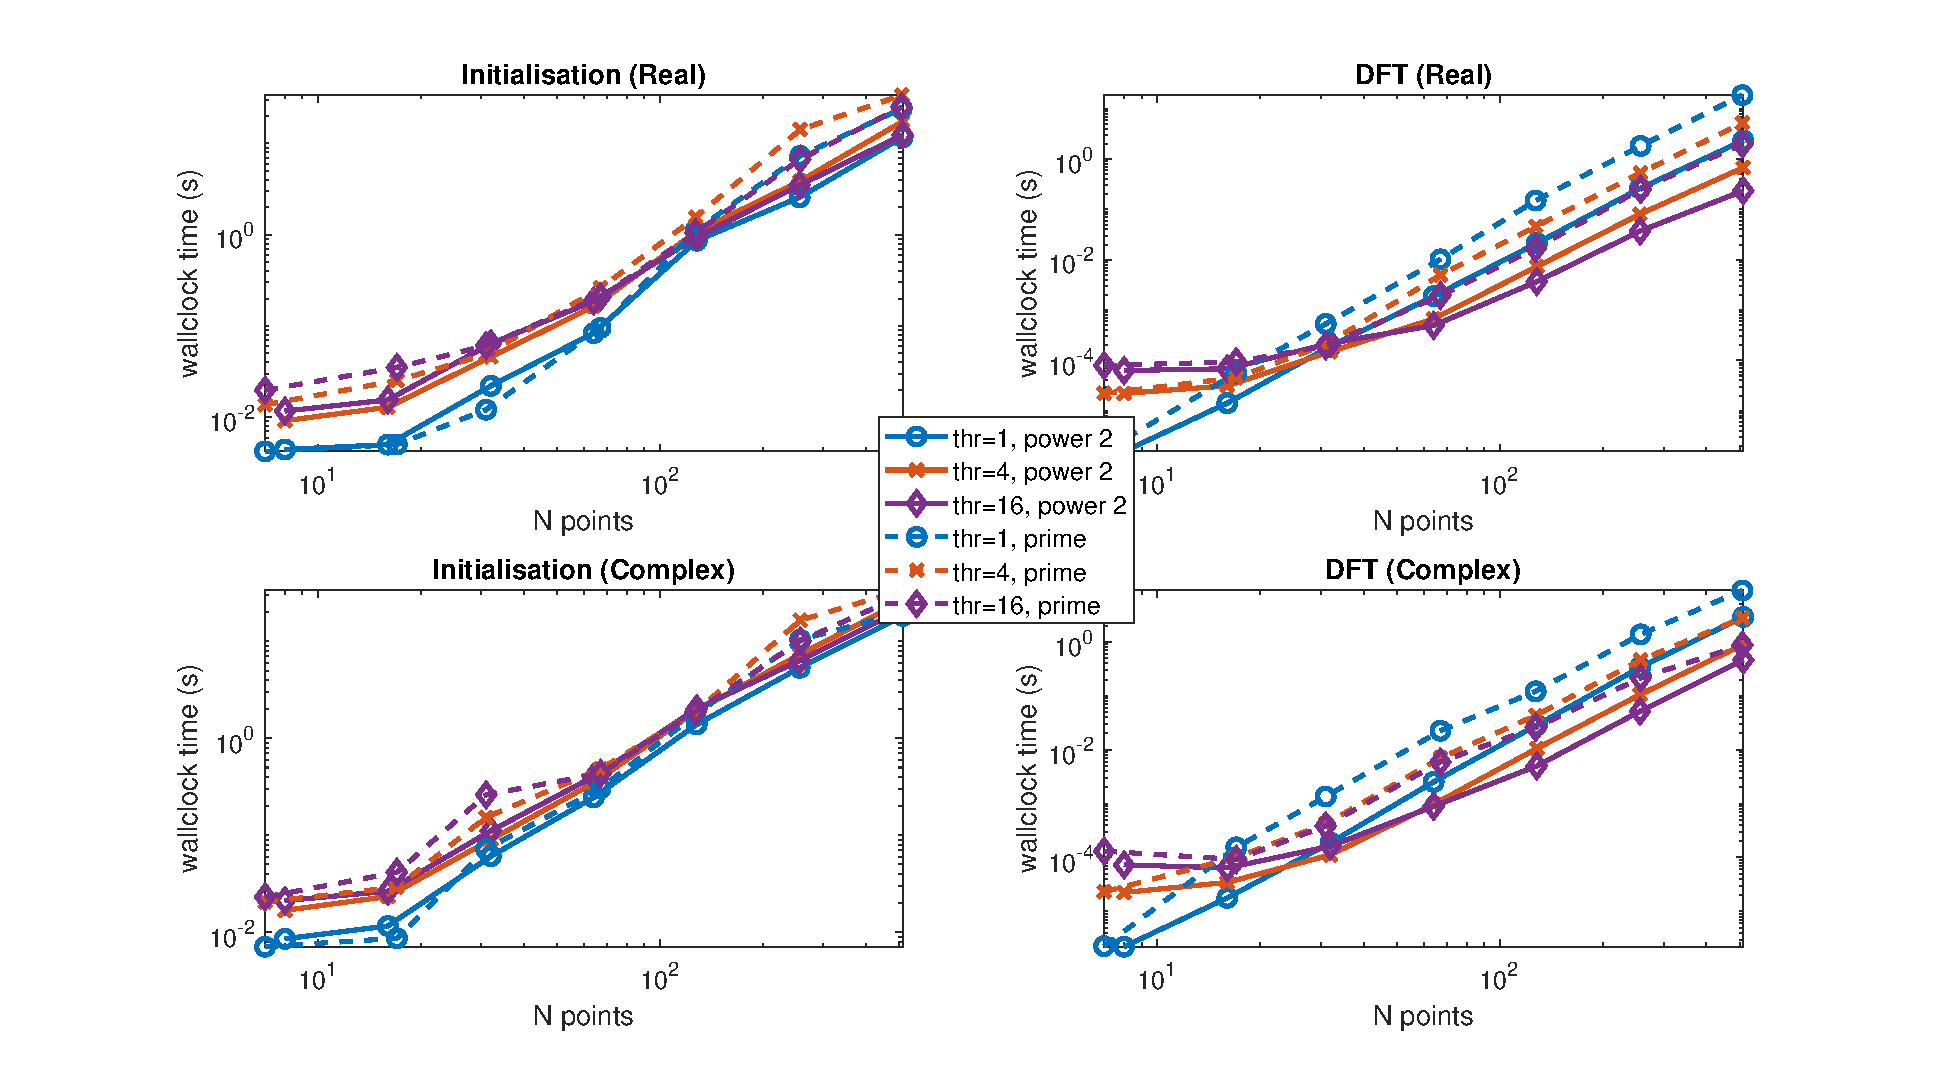
\includegraphics[width=\linewidth]{../results/fftw_3d_thr.eps}
  \caption{Initialisation and DFT execution times of FFTW library applied to 3D signal as a function of the
    number of points, $N,$ and varying the number of threads, $thr.$ }
  \label{3DFFTW}
\end{figure}




\begin{table}
\begin{center}
%\being{small}
\begin{tabular}{|r||r|r||r|r||r|r||r|r|}
  \hline
 & \multicolumn{2}{|c||}{$k(N=31)$} & \multicolumn{2}{|c||}{$k(N=32)$} & \multicolumn{2}{|c||}{$k(N=509)$} & \multicolumn{2}{|c|}{$k(N=512)$} \\
$thr$ &  Real & Complex &  Real & Complex &  Real & Complex &  Real & Complex \\ \hline
  2 & 139  & -  &  825  & 420  & 1 &  6   & 8  & 10 \\
  4 & 114  & -  &  583  & 387  & 1 &  3   & 4  & 4  \\
  8 & 83   & -  &  -    & 353  & 1 &  2   & 2  & 2  \\
  12 & 149 & -  & 14367 & 1176 & 1 &  2   & 4  & 5  \\
  16 & 146 & -  &  -    & 1935 & 1 &  2   & 1  & 2  \\
  24 & 242 & -  &  -    &  -   & 0 &  1   & 3  & 3  \\ \hline
\end{tabular}
\caption{ For $N=31,$ 32, 509 and $N=512,$ the number of DFT calculations, $k,$ required for $thr$ threads to have a lower wallclock time than a single thread when performing  a single initialisation and $k$ DFT calculations are performed with the 3D interface to the FFTW library.  }\label{Tbl:FFTW3dk}
%\end{small}
\end{center}
\end{table}


\subsection{3D MKL Library}\label{Sec:3DMKL}

In Figure~\ref{3DMKL}, we compare the 3D benchmark runs for the MKL
library. As with the 2D runs, we observe that increasing the problem
size has little effect on the initialisation time when a single thread
is used: in this case there is also little difference in
initialisation time when switiching between $N$ being a power of 2 or
prime. When multiple threads are used, the initialisation times drops
significantly as the value of $N$ increases from 7 to 256. For $N=509$
and 512, the initialisation times are very similar to when a single
thread is used. In all cases, the initialisation time decreases when
moving from 4 to 16 threads. For further analysis, we provide the data
for $N=7,$ 8, 64, 67, 509 and 512 in Table~\ref{Tbl:MKL3d}. For $N=7,$
there is a factor of 6 difference in initialisation times when
comparing 1 and 16 threads. For a single thread and real input
signals, increasing $N$ from 7 to 509 increases the initialisation
time by 27\% and increasing $N$ from 8 to 512 increases the
initialisation time by 24\% whilst the overall problem size is
increased by over 5 orders of magnitude; for a single thread with
complex input signals, there are 18\% and 2\% increases in
initialisation times when $N$ increases from 7 to 509 and 8 to 512,
respectively. In comparison, for 16 threads and real input signals,
there are 80\% reductions in initialisation times when switching from
either $N=7$ to 509 or $N=8$ to 512; for complex input signals the
reduction is 77\%.

As expected, increasing $N$ increases the wallclock DFT time and the
time increases when switching from $N$ a power of 2 to the closer
prime number. In Figure~\ref{3DMKL}, we observe that when $N$ is
prime, the DFT decreases as the number of threads increases from 1 to
4 and then to 16 but there appears to be a bigger impact for larger
$N,$ and this is certainly the case for the values of $N$ provided in
Table~\ref{Tbl:MKL3d}. Additionally, multithreading has a lesser
impact when $N$ is a power of 2 than when $N$ is the nearest prime
number to a power of 2.

\begin{figure}[htb]
    \centering
    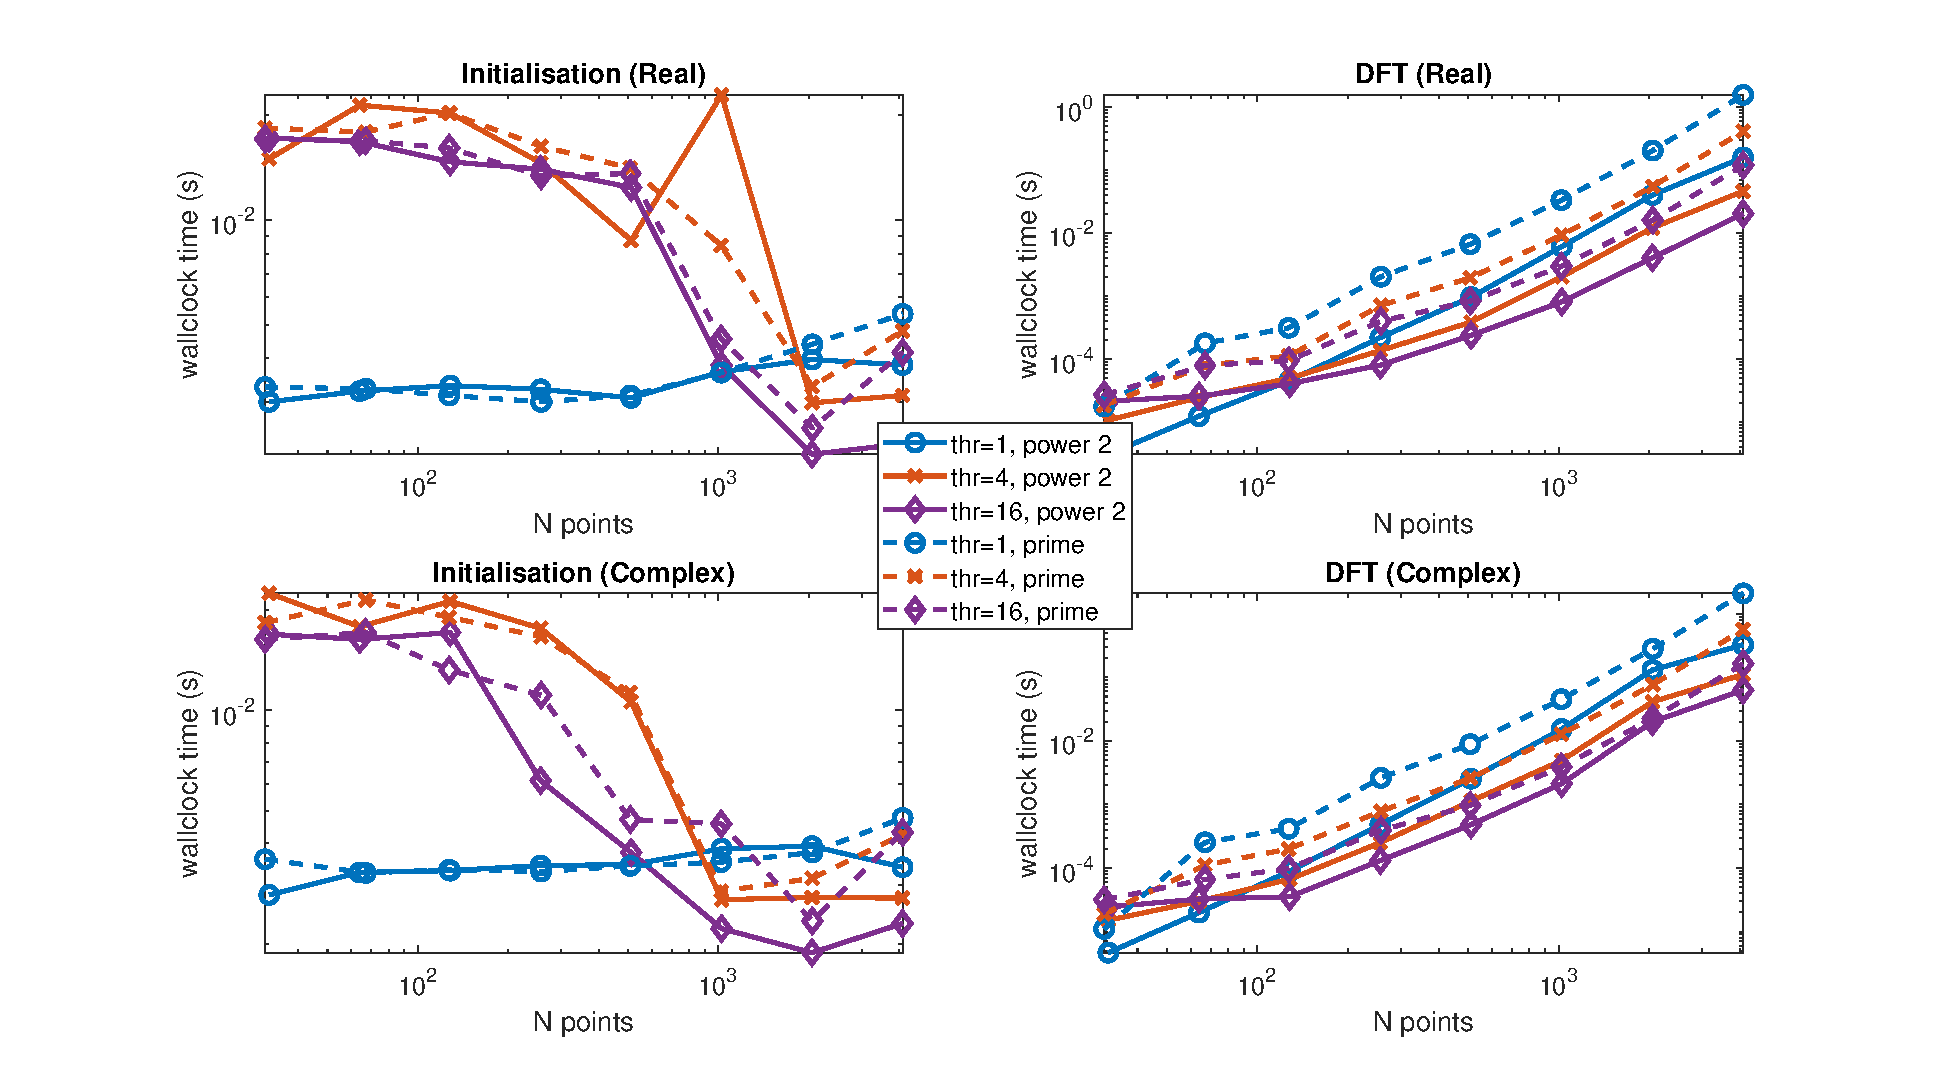
\includegraphics[width=\linewidth]{../results/mkl_3d_thr.eps}
  \caption{Initialisation and DFT execution times of MKL library applied to 3D signal as a function of the
    number of points, $N,$ and varying the number of threads, $thr.$ }
  \label{3DMKL}
\end{figure}





As in Section~\ref{Sec:3DFFTW}, we have calculated the number of DFT
calculations, $k,$ (on average) that would be required for $thr$
threads to have a lower time than a single thread when performing a
single initialisation and $k$ DFT calculations for $N=31,$ 32, 509 and
$N=512:$ these values are provided in
Table~\ref{Tbl:MKL3dk}. Comparing the results for $N=31$ and $N=32,$
multithreading becomes more advantageous far sooner for the prime
value of $N$ and this is primarily because of multithreading having
more affect on the DFT wallclock time. For $N=509$ and $N=512,$ the
use of multiple threads is always advantageous in our benchmark
results.


\begin{table}
\begin{center}
%\being{small}
\begin{tabular}{|r||r|r||r|r||r|r||r|r|}
  \hline
 & \multicolumn{2}{|c||}{$k(N=31)$} & \multicolumn{2}{|c||}{$k(N=32)$} & \multicolumn{2}{|c||}{$k(N=509)$} & \multicolumn{2}{|c|}{$k(N=512)$} \\
$thr$ &  Real & Complex &  Real & Complex  \\ \hline
  2 & 32    & 25  & 446   & 119  & 1 &  1   & 1  &  1 \\
  4 & 48    & 26  & 292   & 225  & 1 &  1   & 1  &  1 \\
  8 & 44    & 26  & 242   & 152  & 1 &  1   & 0  &  1 \\
  12 & 25   & 24  & 193   & 98   & 1 &  1   & 1  &  1 \\
  16 & 24   & 19  & 129   & 91   & 0 &  1   & 1  &  1 \\
  24 & 26   & 17  & 250   & 101  & 1 &  0   & 1  &  1 \\ \hline
\end{tabular}
\caption{ For $N=31,$ 32, 509 and $N=512,$ the number of DFT calculations, $k,$ required for $thr$ threads to have a lower wallclock time than a single thread when performing  a single initialisation and $k$ DFT calculations are performed with the 3D interface to the MKL library.  }\label{Tbl:MKL3dk}
%\end{small}
\end{center}
\end{table}


\subsection{3D P3DFFT Library}\label{Sec:3DP3DFFT}
The P3DFFT library can only take real signals as input: we provide the
benchmark results in Figure~\ref{3DP3DFFT}. The initialisation times
for $N$ a power of 2 are always lower than when $N$ is a prime
number. With the exception of the 3 lowest values of $N$ is the two
different classes of $N,$ in general, multithreading reduces the
initialisation time as we move from 1 to 4 and then 4 to 16
threads. Increasing the problem size increases the initialisation
time. In Table~\ref{Tbl:P3DFFT3d}, we provide the benchmark data for
$N=7,$ 8, 31, 32, 509 and 512. For the largest values of $N$
considered, the effect of multithreading on the wallclock
initialisation time is greater when $N$ is a power 2 than when $N$ is
prime.

Considering the DFT results in Figure~\ref{3DP3DFFT}, when $N$ is a
power of 2 and less than or equal to 64, increasing the number of
threads is also increasing the DFT time; for the larger values of $N$
increasing the number of threads decreases the wallclock DFT time but
there appears to be little difference between 4 and 16 threads,
however, Table~\ref{Tbl:P3DFFT3d} reveals that the DFT time for four
threads is 31\% higher than that of sixteen threads. For prime values
of $N,$ when $N$ is smaller than 31 we observe that increasing the
number of threads increases the DFT time but for larger values of $N$
we get a decrease in DFT time. For $n=509,$ the DFT wallclock time
ratio relative to a single thread is 0.34 for 4 threads, 0.17 for 16
threads and 0.16 for 24 threads. Multithreading has a bigger effect on
DFT time when $N$ is prime compared on $N$ being a power of 2.



\begin{figure}[htb]
    \centering
    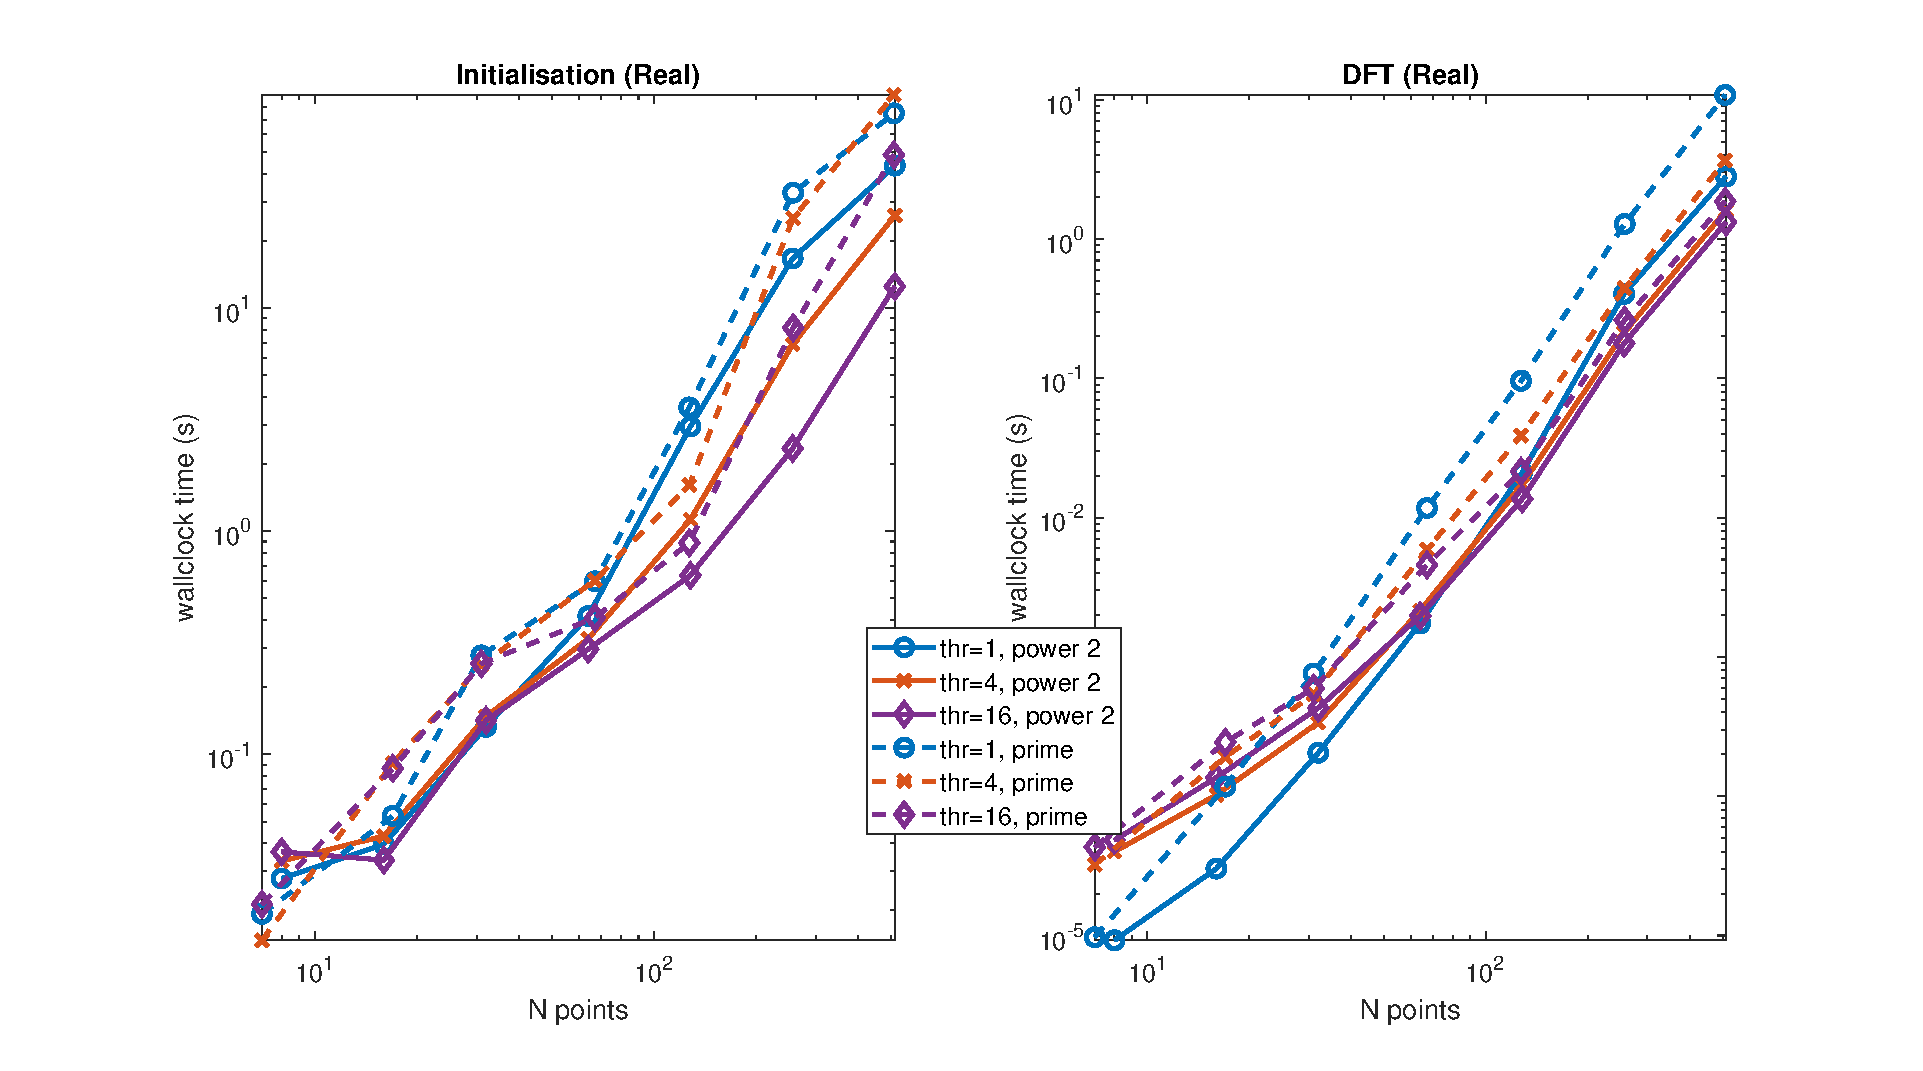
\includegraphics[width=\linewidth]{../results/p3dfft_3d_thr.eps}
  \caption{Initialisation and DFT execution times of P3DFFT library applied to 3D signal as a function of the
    number of points, $N,$ and varying the number of threads, $thr.$ }
  \label{3DP3DFFT}
\end{figure}







\subsection{Comparison of libraries for 3D benchmarks}\label{Sec:3DComp}

We compare the initialisation and DFT wallclock times for FFTW, MKL
and P3DFFT in Figures~\ref{3DFFTWMKL2} ($N$ a power of 2) and
\ref{3DFFTWMKLPrime} ($N$ prime). For all cases, MKL is the fastest in
terms of initialisation time and P3DFFT is, in general, the slowest in
the real input signal cases. The differences are generally significant
and, using the data from Tables~\ref{Tbl:FFTW3d}, \ref{Tbl:MKL3d} and
\ref{Tbl:P3DFFT3d}, we provide the ratio of initialisation and DFT
times for FFTW and P3DFFT with respect to the MKL library in
Tables~\ref{Tbl:Init3dr}, \ref{Tbl:Init3dc}, \ref{Tbl:DFT3dr} and
\ref{Tbl:DFT3dr}. In the real case (Table~\ref{Tbl:Init3dr}), we see
that the FFTW and P3DFFT initialisation time ratios are higher for
$N=509$ than for $N=512,$ and the ratios are very large. For the two
smallest values of $N,$ the initialisation times for the real case are
comparable for all the libraries when a large number of threads are
used but, for a small number of threads, we note that the difference
is much greater for P3DFFT than for FFTW. In the complex case
(Table~\ref{Tbl:Init3dc}), the initialisation ratios are similar to
those of the real case for the FFTW library.

Considering the real case and DFT times, we observe that increasing
the number of threads generally increases the ratio of P3DFFT relative
to MKL, whilst the ratios remain similar for the FFTW library when $N$ is
large: this is also the case for complex input signals.

Combining all of these comparisons together, we conclude that the MKL
library is, in general, outperforming both the FFTW and P3DFFT
libraries.




\begin{figure}[htb]
    \centering
    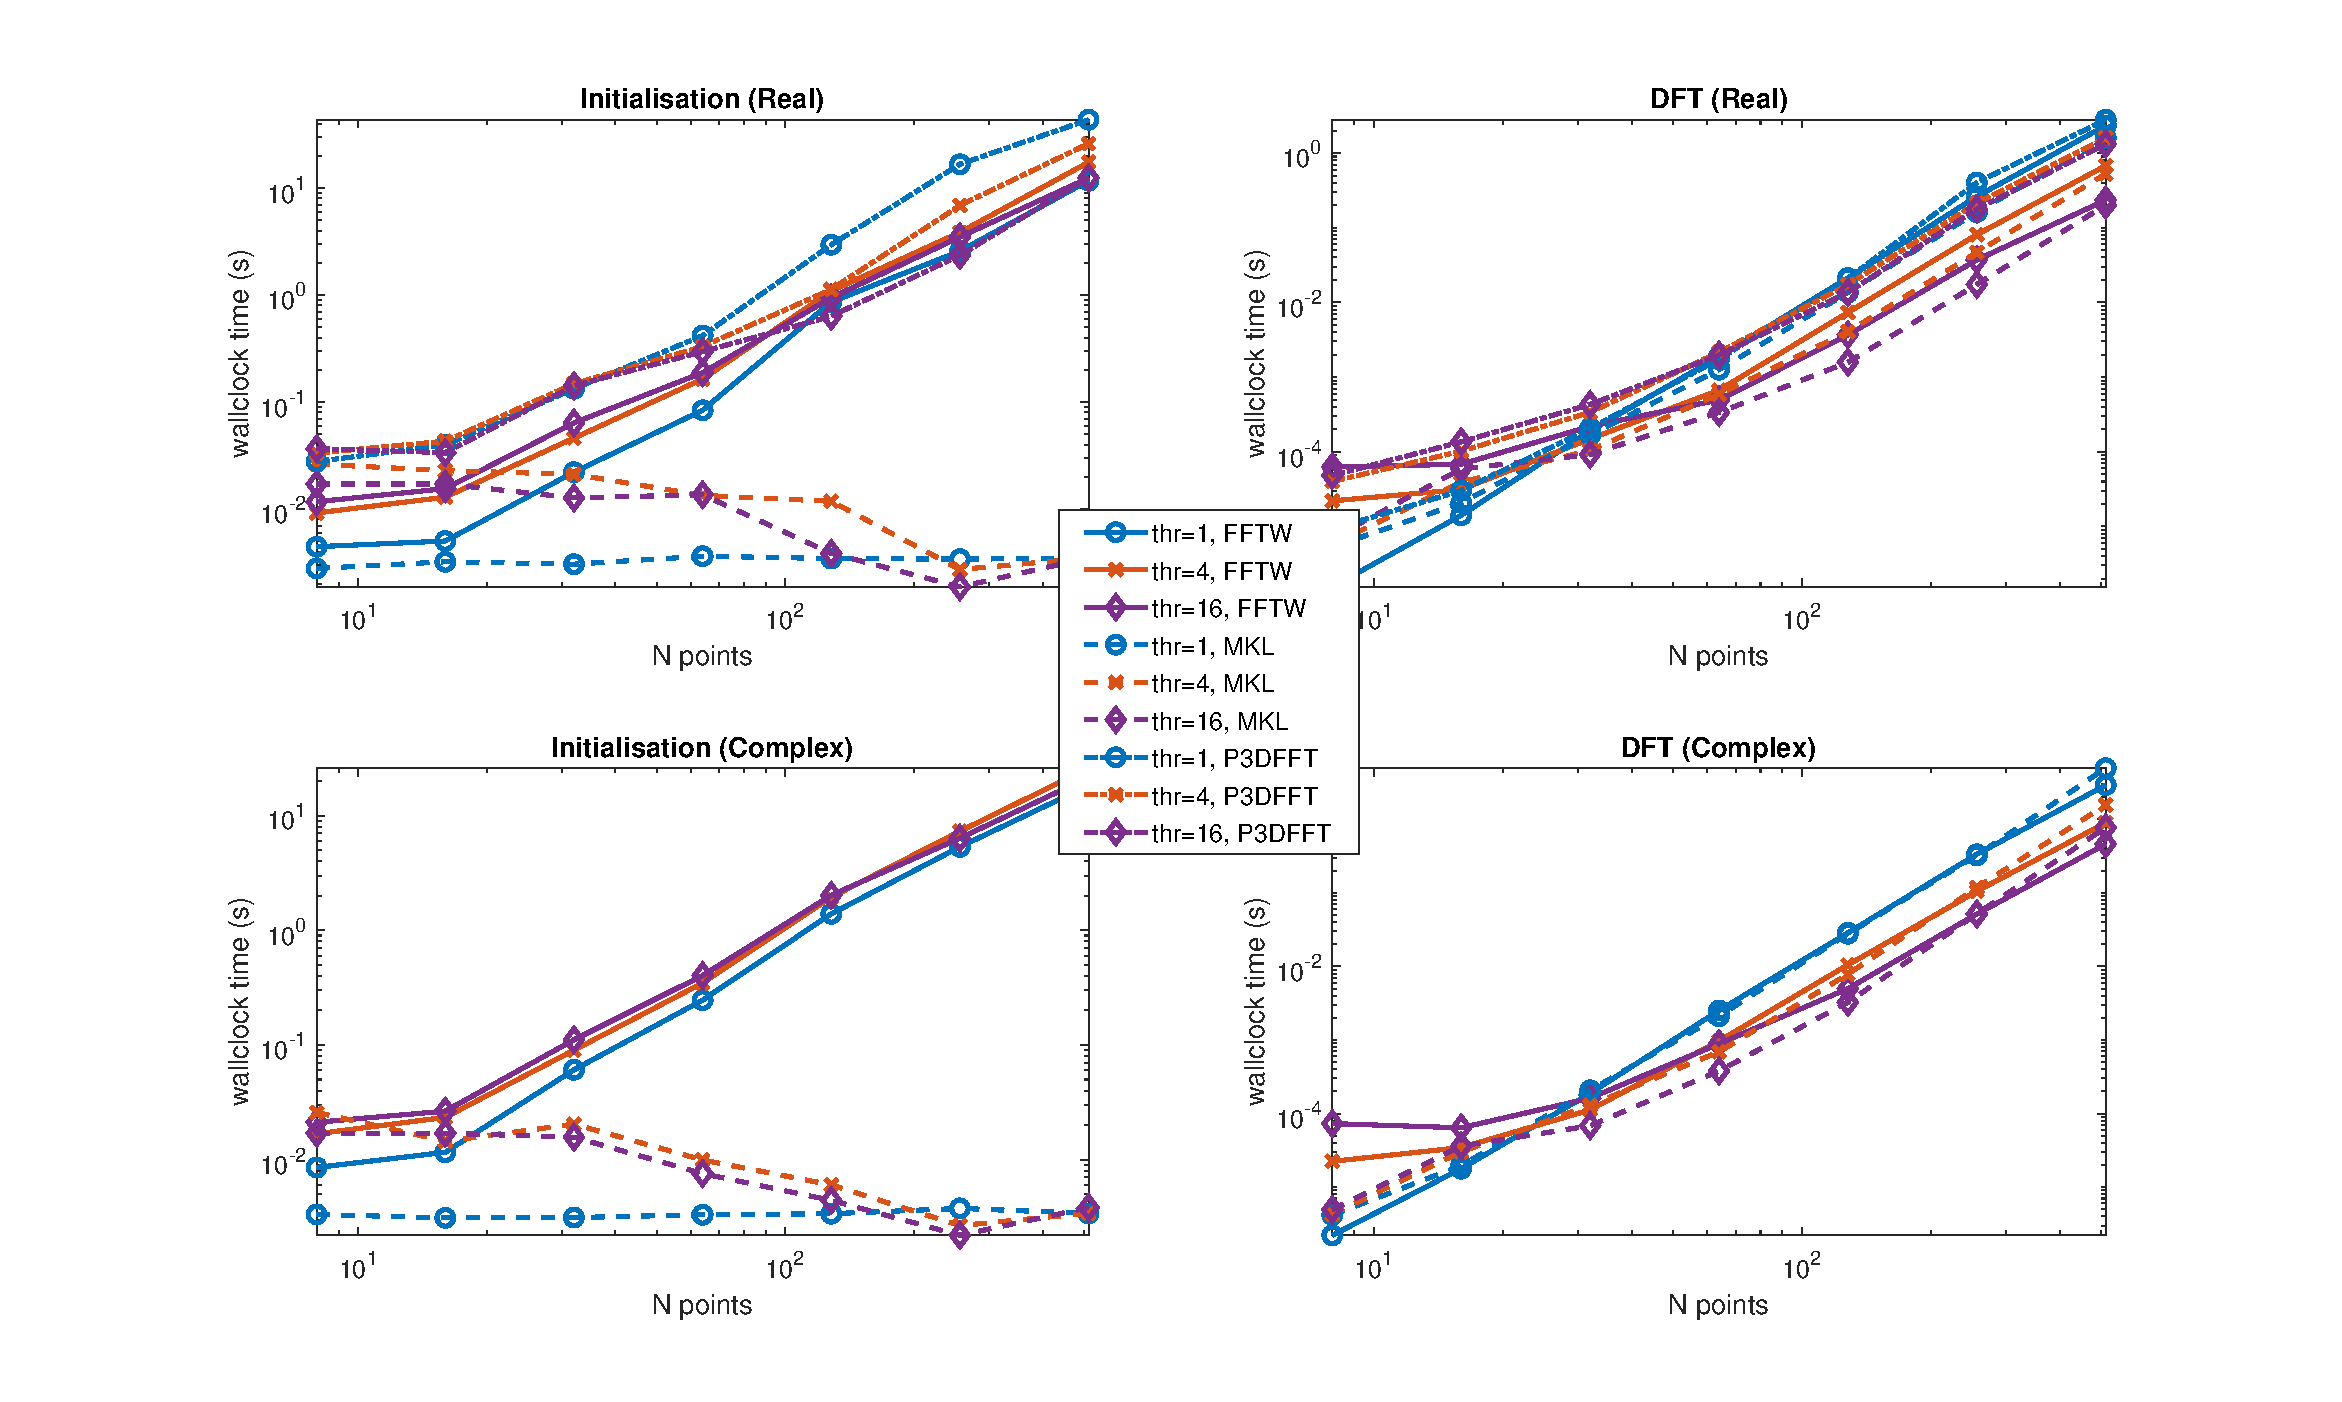
\includegraphics[width=\linewidth]{../results/fftw_mkl_p3dfft_2_3d_thr.eps}
  \caption{Initialisation and DFT execution times of FFTW, MKL and P3DFFT libraries applied to 3D signal as a function of the
    number of points, $N,$ and varying the number of threads, $thr.$ $N$ is a power of 2.}
  \label{3DFFTWMKL2}
\end{figure}


\begin{figure}[htb]
    \centering
    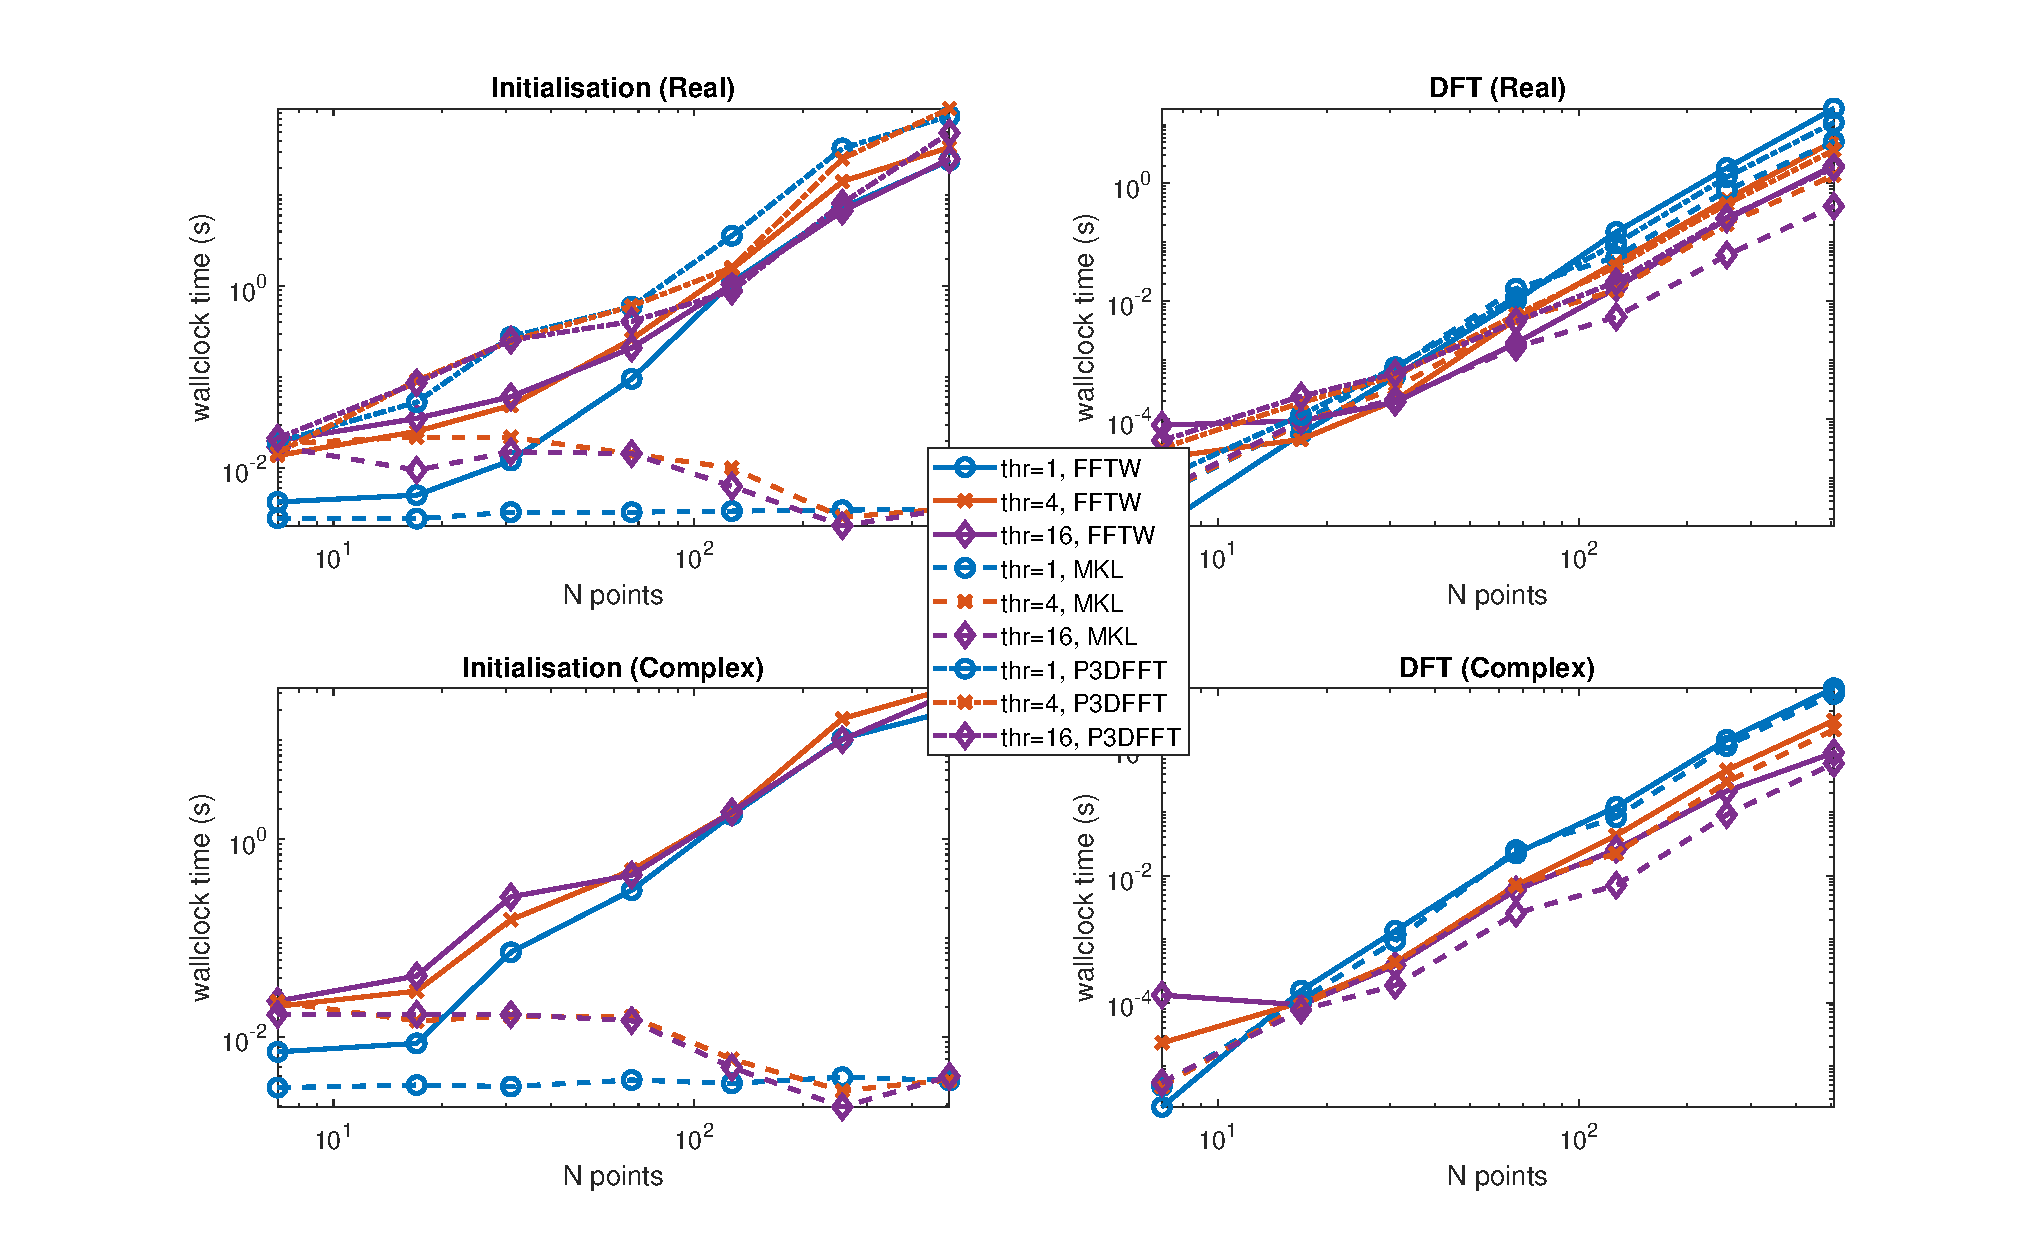
\includegraphics[width=\linewidth]{../results/fftw_mkl_p3dfft_prime_3d_thr.eps}
  \caption{Initialisation and DFT execution times of FFTW, MKL and P3DFFT libraries applied to 3D signal as a function of the
    number of points, $N,$ and varying the number of threads, $thr.$ $N$ is a prime number.}
  \label{3DFFTWMKLPrime}
\end{figure}

\begin{table}
\begin{center}
%\being{small}
\begin{tabular}{|r||r|r||r|r||r|r||r|r|}
  \hline
  &    \multicolumn{2}{|c||}{$N=7$} & \multicolumn{2}{|c||}{$N=8$} & \multicolumn{2}{|c||}{$N=509$} & \multicolumn{2}{|c|}{$N=512$}  \\
$thr$  & FFTW & P3DFFT & FFTW & P3DFFT & FFTW & P3DFFT & FFTW & P3DFFT  \\  \hline 
   1  &   1.51e+0 &   6.87e+0 &   1.60e+0 &   1.00e+1 &   6.80e+3 &   2.10e+4 &   3.38e+3 &   1.26e+4   \\
   2  &   4.13e+0 &   7.88e+0 &   3.25e+0 &   1.35e+1 &   8.78e+3 &   2.81e+4 &   5.20e+3 &   9.28e+3   \\
   4  &   7.41e-1 &   7.95e-1 &   3.49e-1 &   1.27e+0 &   9.44e+3 &   2.52e+4 &   5.00e+3 &   7.47e+3   \\
   8  &   1.21e+0 &   1.23e+0 &   2.88e-1 &   7.93e-1 &   6.11e+3 &   1.68e+4 &   4.55e+3 &   5.68e+3   \\
   12 &   1.49e+0 &   1.30e+0 &   9.55e-1 &   2.12e+0 &   8.61e+3 &   1.62e+4 &   5.23e+3 &   9.38e+3   \\
   16 &   1.15e+0 &   1.24e+0 &   6.84e-1 &   2.14e+0 &   7.04e+3 &   1.37e+4 &   3.55e+3 &   3.58e+3   \\
   24 &   1.34e+0 &   1.28e+0 &   1.37e+0 &   1.94e+0 &   5.93e+3 &   9.80e+3 &   5.03e+3 &   5.62e+3   \\ \hline
\end{tabular}
\caption{ For $N=7,$ 8, 509 and $N=512,$ the ratio of initialisation time for FFTW and P3DFFT with respect to the MKL library  with real input signals. }\label{Tbl:Init3dr}
%\end{small}
\end{center}
\end{table}

\begin{table}
\begin{center}
%\being{small}
\begin{tabular}{|r|r|r|r|r|}
  \hline
  $thr$ & $N=7$ & $N=8$ & $N=509$ & $N=512$ \\ \hline
   1  &      2.29e+0 &   2.57e+0 &   5.40e+3 &   5.38e+3  \\
   2  &      1.37e+0 &   6.14e+0 &   1.16e+4 &   8.56e+3  \\
   4  &      9.07e-1 &   6.51e-1 &   9.03e+3 &   7.57e+3  \\
   8  &      1.45e+0 &   7.58e-1 &   8.09e+3 &   6.35e+3  \\
   12 &      1.41e+0 &   1.49e+0 &   8.80e+3 &   8.83e+3  \\
   16 &      1.37e+0 &   1.25e+0 &   7.36e+3 &   5.61e+3  \\
   24 &      1.24e+0 &   1.37e+0 &   6.85e+3 &   7.30e+3  \\ \hline
\end{tabular}
\caption{ For $N=7,$ 8, 509 and $N=512,$ the ratio of initialisation time for FFTW with respect to the MKL library  with complex signals. }\label{Tbl:Init3dc}
%\end{small}
\end{center}
\end{table}

\begin{table}
\begin{center}
%\being{small}
\begin{tabular}{|r||r|r||r|r||r|r||r|r|}
  \hline
  &    \multicolumn{2}{|c||}{$N=7$} & \multicolumn{2}{|c||}{$N=8$} & \multicolumn{2}{|c||}{$N=509$} & \multicolumn{2}{|c|}{$N=512$}  \\
 $thr$  & FFTW & P3DFFT & FFTW & P3DFFT & FFTW & P3DFFT & FFTW & P3DFFT   \\  \hline 
   1  &   2.95e-1 &   1.85e+0 &   2.92e-1 &   1.74e+0 &   3.62e+0 &   2.09e+0 &   1.48e+0 &   1.77e+0  \\
   2  &   1.97e+0 &   4.49e+0 &   3.50e+0 &   5.05e+0 &   3.76e+0 &   2.32e+0 &   1.40e+0 &   2.34e+0   \\
   4  &   3.99e+0 &   5.81e+0 &   3.81e+0 &   6.92e+0 &   3.82e+0 &   2.65e+0 &   1.28e+0 &   3.03e+0   \\
   8  &   5.36e+0 &   6.25e+0 &   4.46e+0 &   8.14e+0 &   4.28e+0 &   3.36e+0 &   1.13e+0 &   4.29e+0   \\
   12 &   6.33e+0 &   6.33e+0 &   1.38e+1 &   6.93e+0 &   3.84e+0 &   4.03e+0 &   1.14e+0 &   5.20e+0  \\
   16 &   1.31e+1 &   7.16e+0 &   9.01e+0 &   6.93e+0 &   4.84e+0 &   4.53e+0 &   1.17e+0 &   6.57e+0   \\
   24 &   1.43e+1 &   6.48e+0 &   8.76e+0 &   6.26e+0 &   3.54e+0 &   4.90e+0 &   1.46e+0 &   7.74e+0    \\ \hline
\end{tabular}
\caption{ For $N=7,$ 8, 509 and $N=512,$ the ratio of DFT time with respect to the MKL library for FFTW and P3DFFT. }\label{Tbl:DFT3dr}
%\end{small}
\end{center}
\end{table}

\begin{table}
\begin{center}
%\being{small}
\begin{tabular}{|r||r|r|r|r|}
  \hline
  &   $N=7$ & $N=8$ & $N=509$ & $N=512$ \\ \hline
   1  &     4.68e-1 &   5.30e-1 &   1.23e+0 &   5.87e-1  \\
   2  &     2.83e+0 &   4.96e+0 &   1.29e+0 &   5.32e-1  \\
   4  &     4.84e+0 &   5.22e+0 &   1.39e+0 &   5.72e-1  \\
   8  &     3.42e+1 &   9.62e+0 &   1.36e+0 &   5.34e-1  \\
   12 &     1.52e+1 &   2.93e+1 &   1.39e+0 &   6.00e-1  \\
   16 &     2.39e+1 &   1.47e+1 &   1.48e+0 &   5.97e-1  \\
   24 &     2.97e+1 &   3.20e+1 &   1.34e+0 &   5.97e-1  \\ \hline
\end{tabular}
\caption{ For $N=7,$ 8, 509 and $N=512,$ the ratio of DFT time with respect to the MKL library for FFTW and P3DFFT. }\label{Tbl:DFTd3dc}
%\end{small}
\end{center}
\end{table}


\section{Effect of domain size and distributed parallelisation for 1D benchmarks}\label{Sec:1DDistr}
In this section, we discuss the benchmark results for distributed
libraries that apply the fast Fourier transform to 1D arrays.  The
P3DFFT library cannot be used on 1D problems and, hence, is
excluded. These benchmarks were performed with the MPI-OpenMP versions
of FFTW and MKL. 

As in Section~\ref{Sec:1DMulti}, we set $n_2=4,$ $n_q=4$ and $n_1=N,$ were $N$ is
defined as follows.  For one set of tests, we let $N=2^k$ for
$k=8,\ldots,20.$ For the other set of tests, $N$ is defined to be the
closest prime number to $2^k,$ $k=8,\ldots,20:$ if two primes are
equidistant, we choose the larger one.

\subsection{1D Distributed FFTW Library}\label{Sec:1DDistFFTW}

The distributed version of the FFTW library only
provides a 1D interface for complex input signals. As with the
multithreaded benchmark results, we are restricted to values of $N$
that are at most $2^{14}.$ We also found that the library had a bug
when 12 or 24 MPI processes where requested and would crash.

In Figure~\ref{1DDistFFTW}, we compare our benchmark results for 1, 4
and 16 MPI processes, $P,$ with a single thread per process. When
$P=16,$ we observe a bump in the initialisation times at $N=1024:$
further analysis of the benchmark data revealed that this bump was
replicated across all of the benchmark runs. For the larger values of
$N,$ increasing the number of processes decreases the initialisation
times when $N$ is a power of 2 but there is little change when $N$ is
prime. Looking at DFT times, when $N$ is a power of 2, we observe an
increase in wallclock time as we increase the number of processes in
all but the larger values of $N$ but the restriction in size of $N$
means that we are barely seeing any advantage in using multiple
processes. When $N$ is prime, increasing the number of processes
results in a small increase in DFT wallclock time.


\begin{figure}[htb]
    \centering
    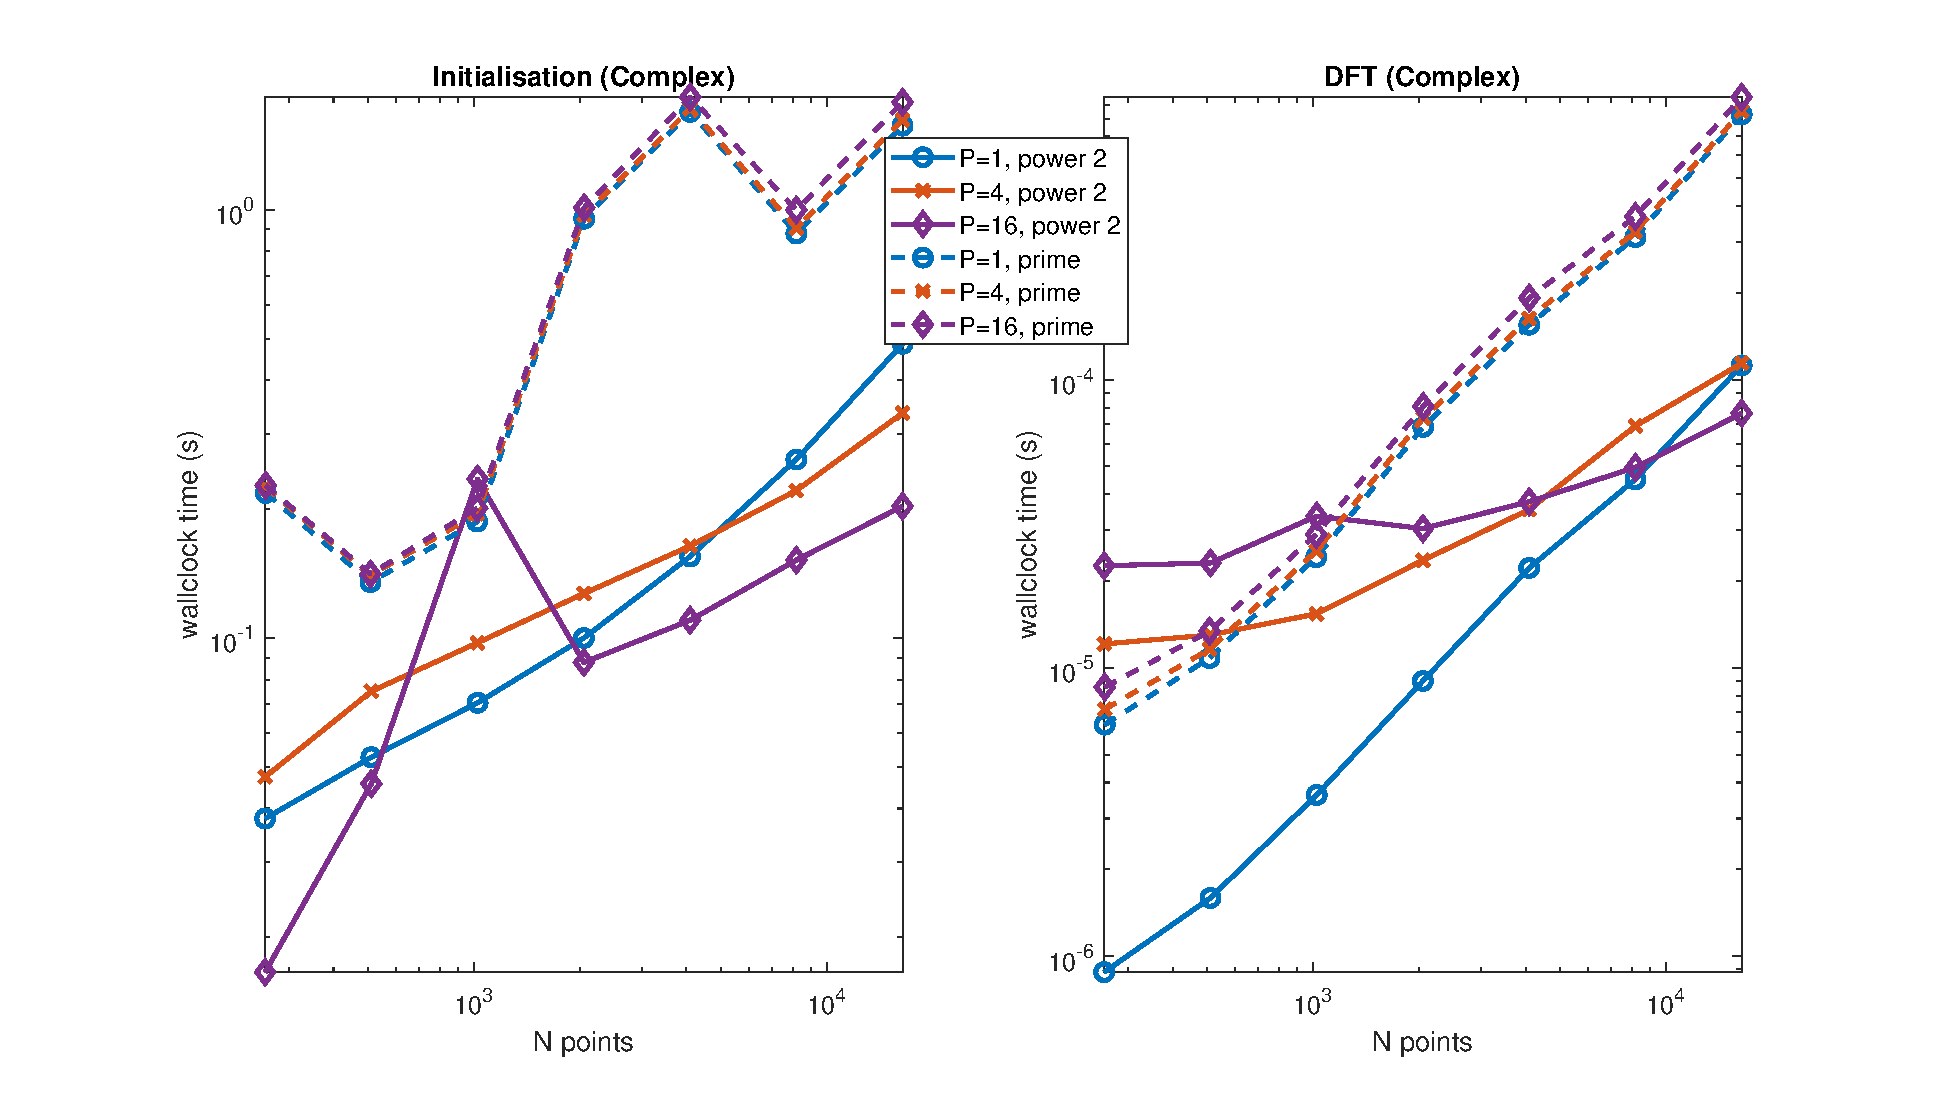
\includegraphics[width=\linewidth]{../results/fftw_1d_mpi.eps}
  \caption{Initialisation and DFT execution times of distributed FFTW library applied to 1D signal as a function of the
    number of points, $N,$ and varying the number of MPI processes, $P,$ with one thread per process.}
  \label{1DDistFFTW}
\end{figure}

In Figure~\ref{1DDistFFTW16}, we compare our benchmark test results
when $P\times thr=16$ and $P=1,$ 4 and 16, and observe that it was, in
general, better to use a single thread with 16 MPI processes in the
benchmarks compared. For $N=16381,$ we provide all of the data and
ratios relative to using $P=1$ and $thr=1$ in
Table~\ref{Tbl:FFT1d16381} and find that the combination of one MPI
process with four threads was optimal. In Table~\ref{Tbl:FFT1d16384}
we provide the data for $N=16384$ and discover that 16 MPI processes
and a single thread per MPI process was optimal. However, we cannot
take $N$ large enough to find a general trend.

\begin{figure}[htb]
    \centering
    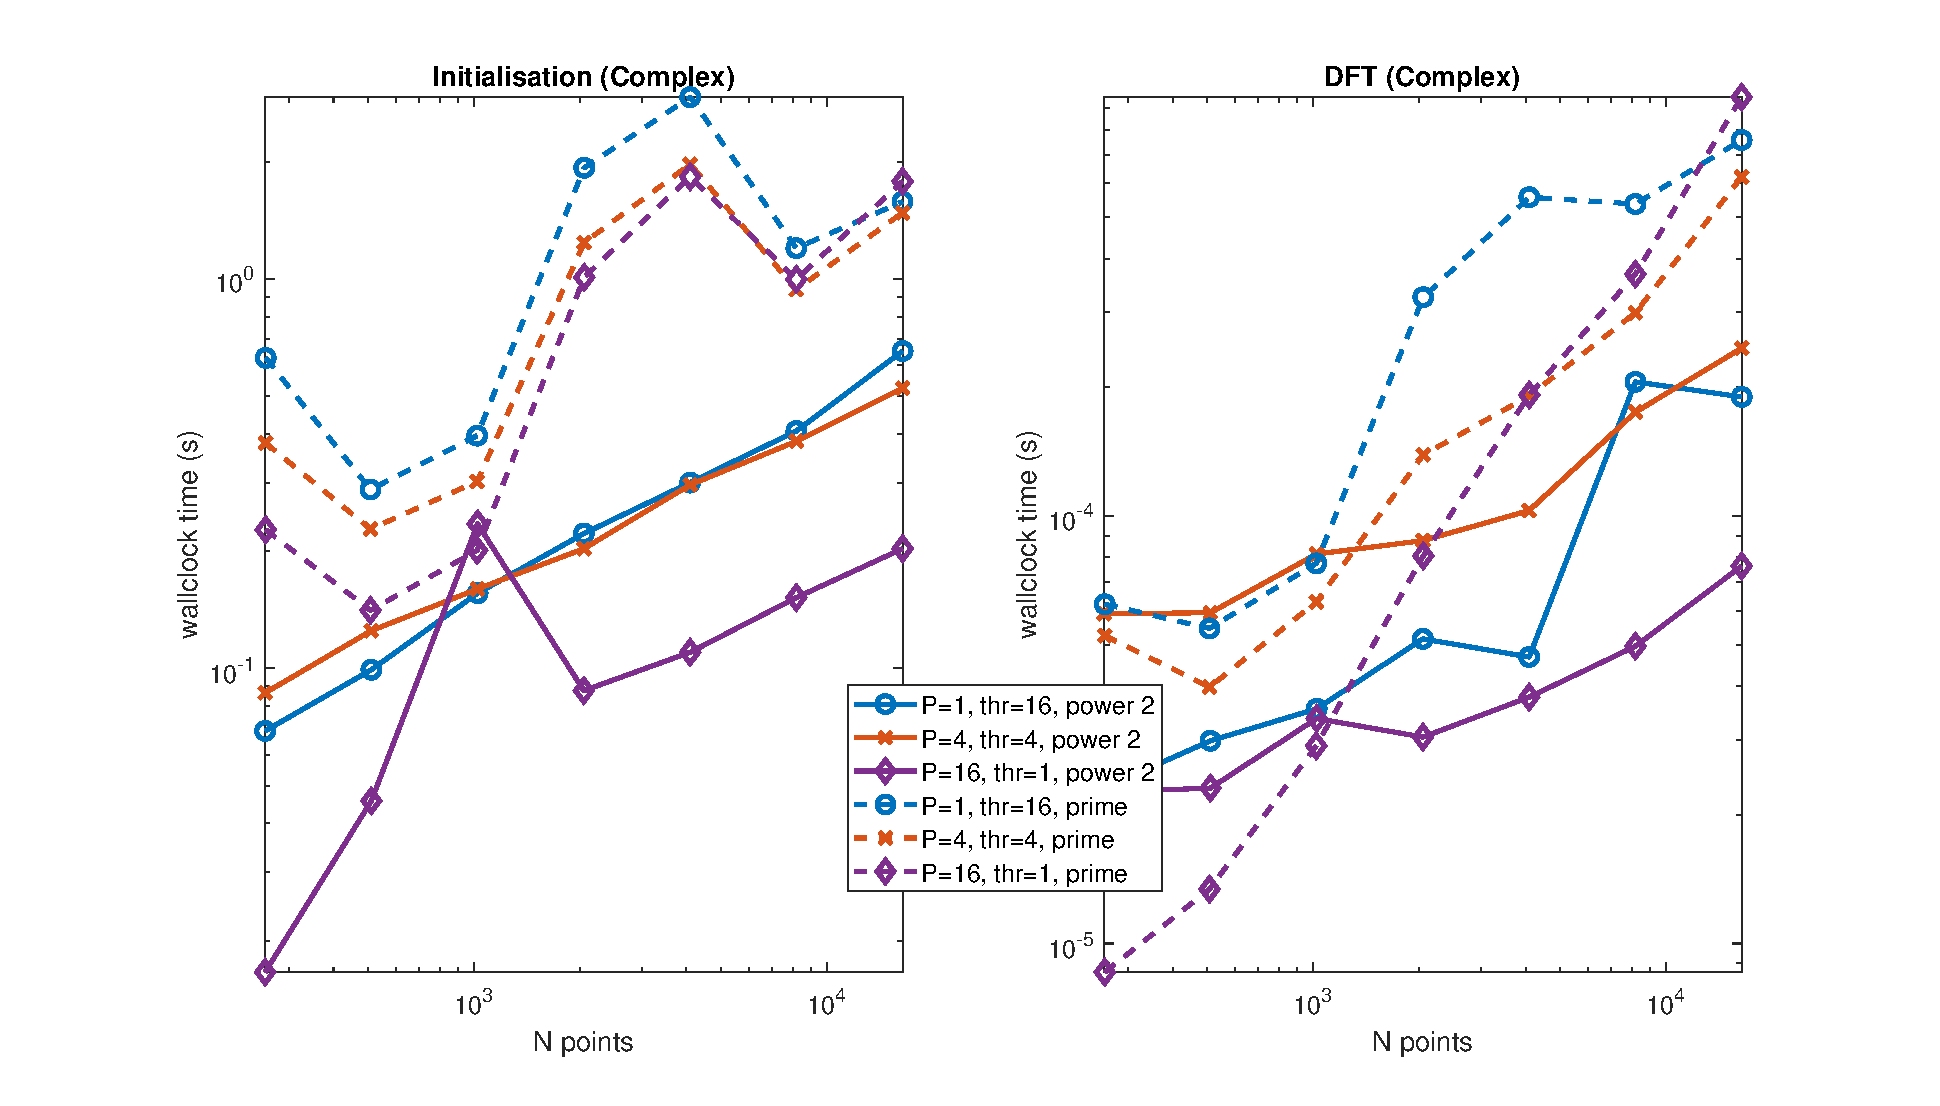
\includegraphics[width=\linewidth]{../results/fftw_1d_mpi_thr.eps}
  \caption{Initialisation and DFT execution times of distributed FFTW library applied to 1D signal as a function of the
    number of points, $N,$ and varying the number of MPI processes, $P,$ and threads, $thr,$ whilst maintaining $P\times thr=16.$}
  \label{1DDistFFTW16}
\end{figure}









\subsection{1D Distributed MKL Library}\label{Sec:1DDistMKL}
In contrast to the distributed FFTW library, the distributed MKL
library has 1D interfaces for both real and complex input
signals. However, the interface does not allow prime values of $N.$


Using one thread per MPI process, we compare our benchmark results for
$P=1,$ 4 and 16 in Figure~\ref{1DDistMKL}. For $N<10^4,$ the
initialisation times remain almost constant as the size of $N$
increases with $P=4$ having an initialisation time that is roughly 15
times larger than that of a single process and $P=16$ being roughly 30
times larger that the single process, with the real and complex
benchmarks having very similar values. In Table~\ref{Tbl:MKL1d16384},
we provide the data for $N=16384$ and ratios with respect to $P=1$ and
$thr=1.$ We start by observing that, for a single thread per MPI
process, increasing the number of processes has a larger effect on
initialisation time when the input signal is real instead of being
complex and, hence, the initialisation times are slightly lower for
the complex case when a large number of processes are used. For
$N>10^4,$ the difference in initialisation times for different numbers
of MPI processes appears to narrow in Figure~\ref{1DDistMKL}: the data
for $N=1048576$ is provided for in Table~\ref{Tbl:MKL1d1048576} and
the values of iratio are much lower than those in
Table~\ref{Tbl:MKL1d16384} but increasing the number of processes
still, in general, increases the initialisation times.

Comparing the DFT wallclock execution times in Figure~\ref{1DDistMKL}



\begin{figure}[htb]
    \centering
    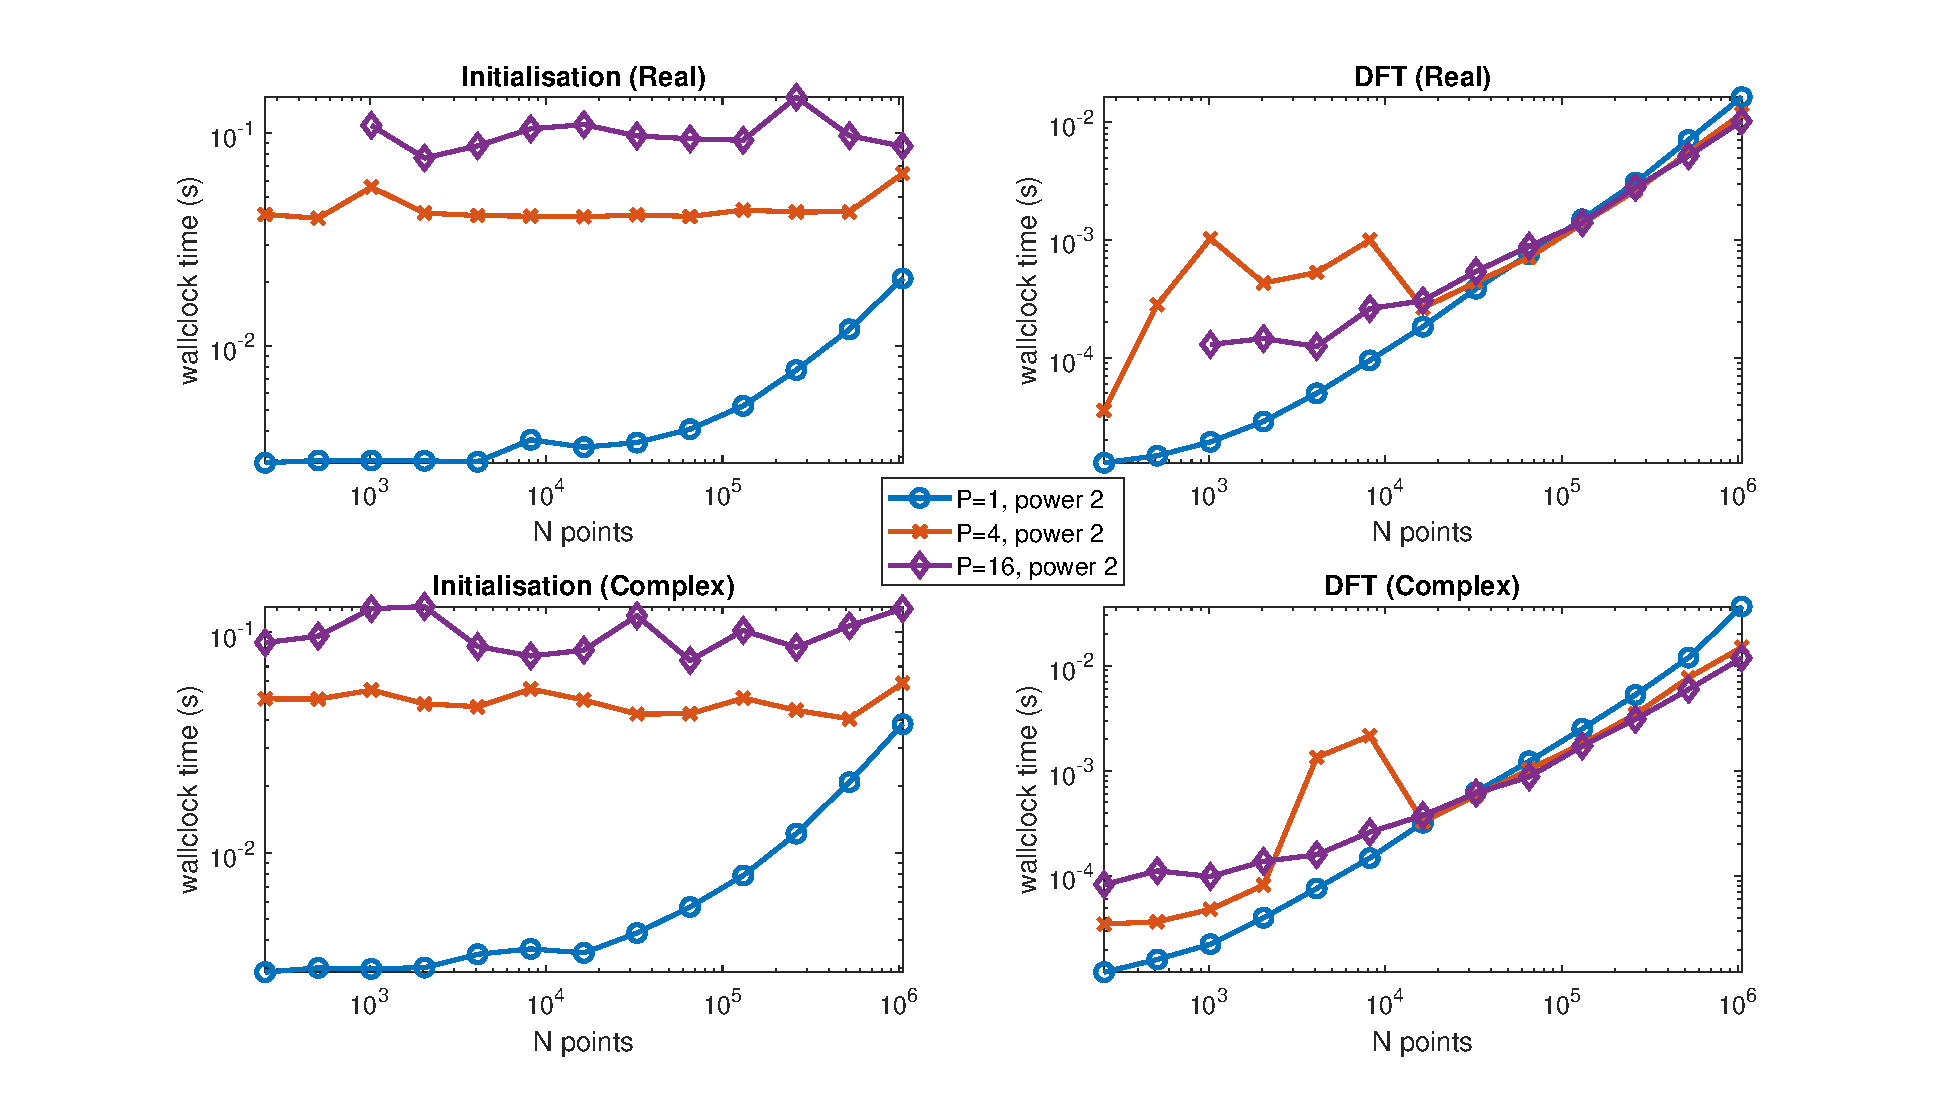
\includegraphics[width=\linewidth]{../results/mkl_1d_mpi.eps}
  \caption{Initialisation and DFT execution times of distributed MKL library applied to 1D signal as a function of the
    number of points, $N,$ and varying the number of MPI processes, $P,$ with one thread per process.}
  \label{1DDistMKL}
\end{figure}

\begin{figure}[htb]
    \centering
    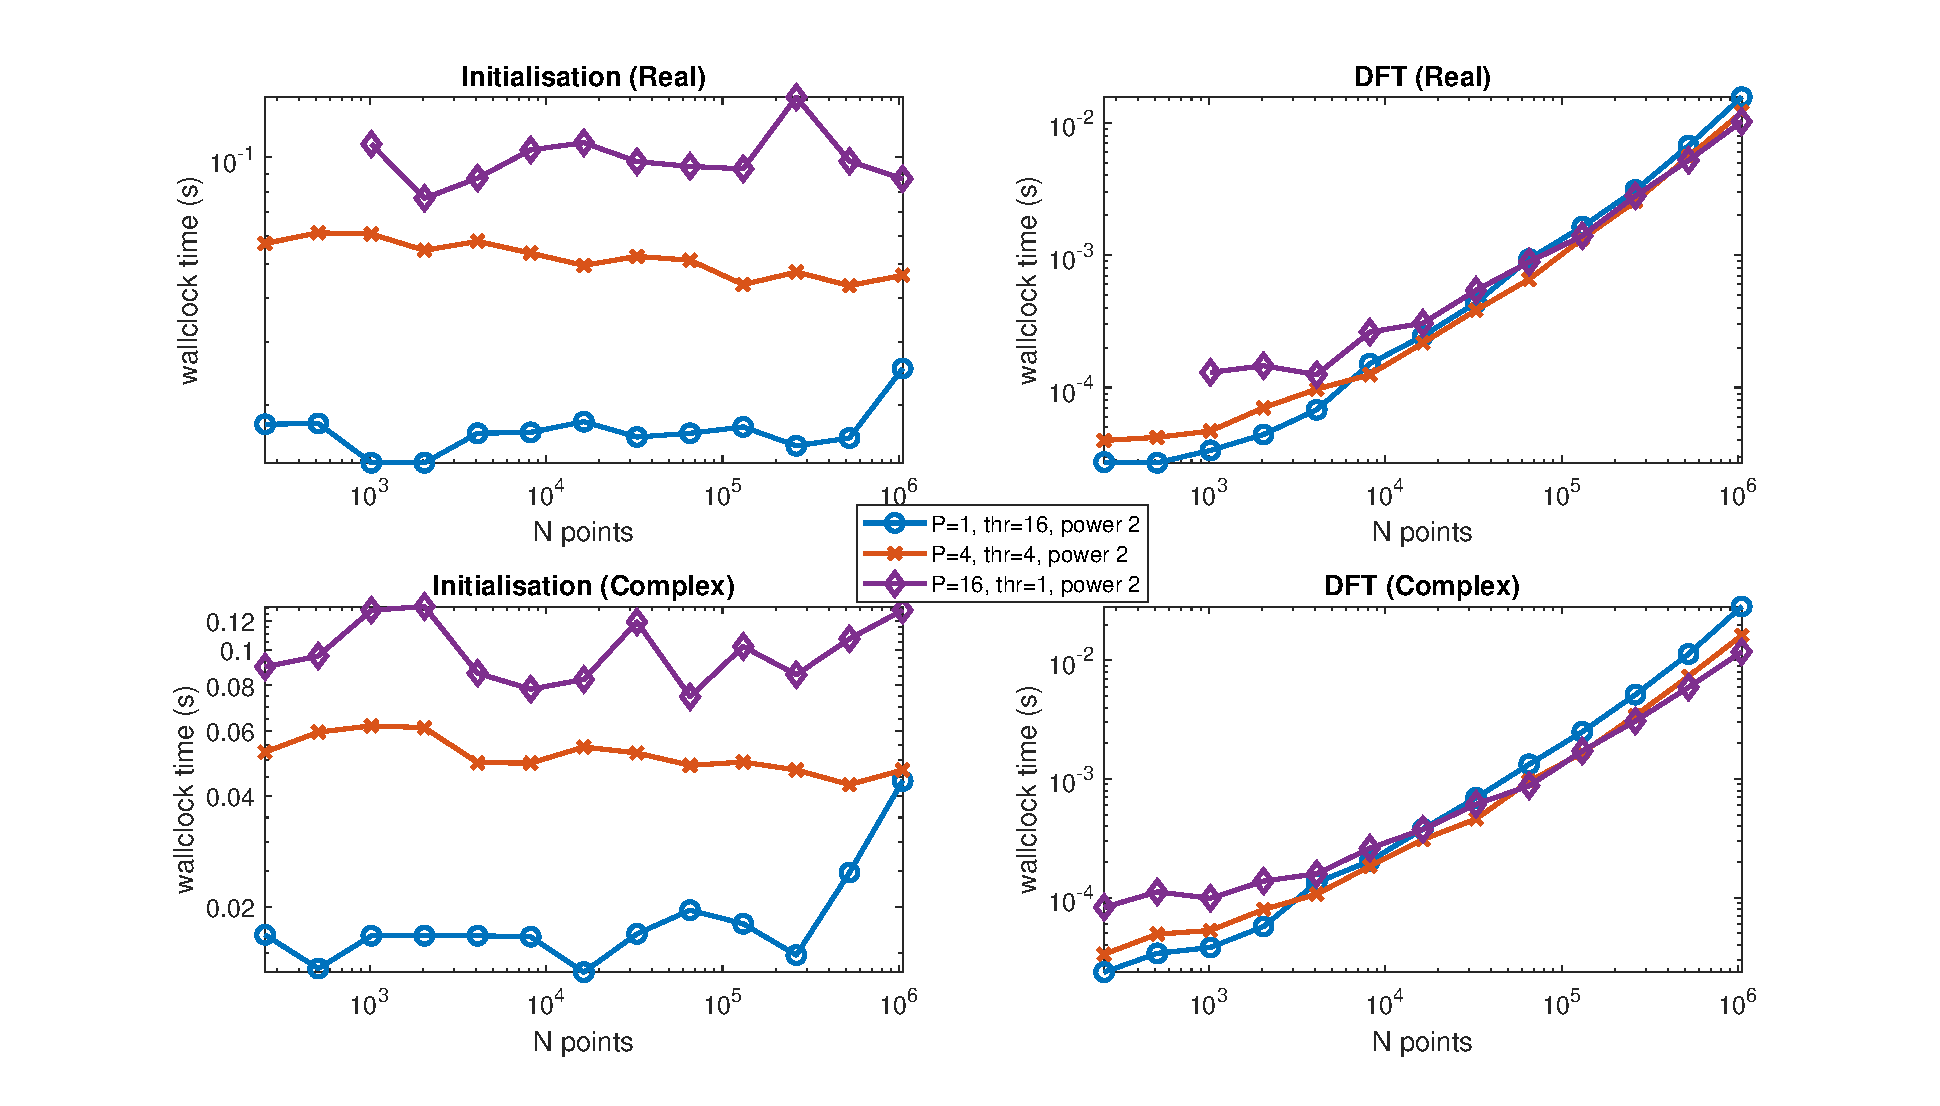
\includegraphics[width=\linewidth]{../results/mkl_1d_mpi_thr.eps}
  \caption{Initialisation and DFT execution times of distributed MKL library applied to 1D signal as a function of the
    number of points, $N,$ and varying the number of MPI processes, $P,$ and threads, $thr,$ whilst maintaining $P\times thr=16.$}
  \label{1DDistMKL16}
\end{figure}






\subsection{Comparison of distributed libraries for 1D benchmark}\label{Sec:1DDistComp}


\begin{figure}[htb]
    \centering
    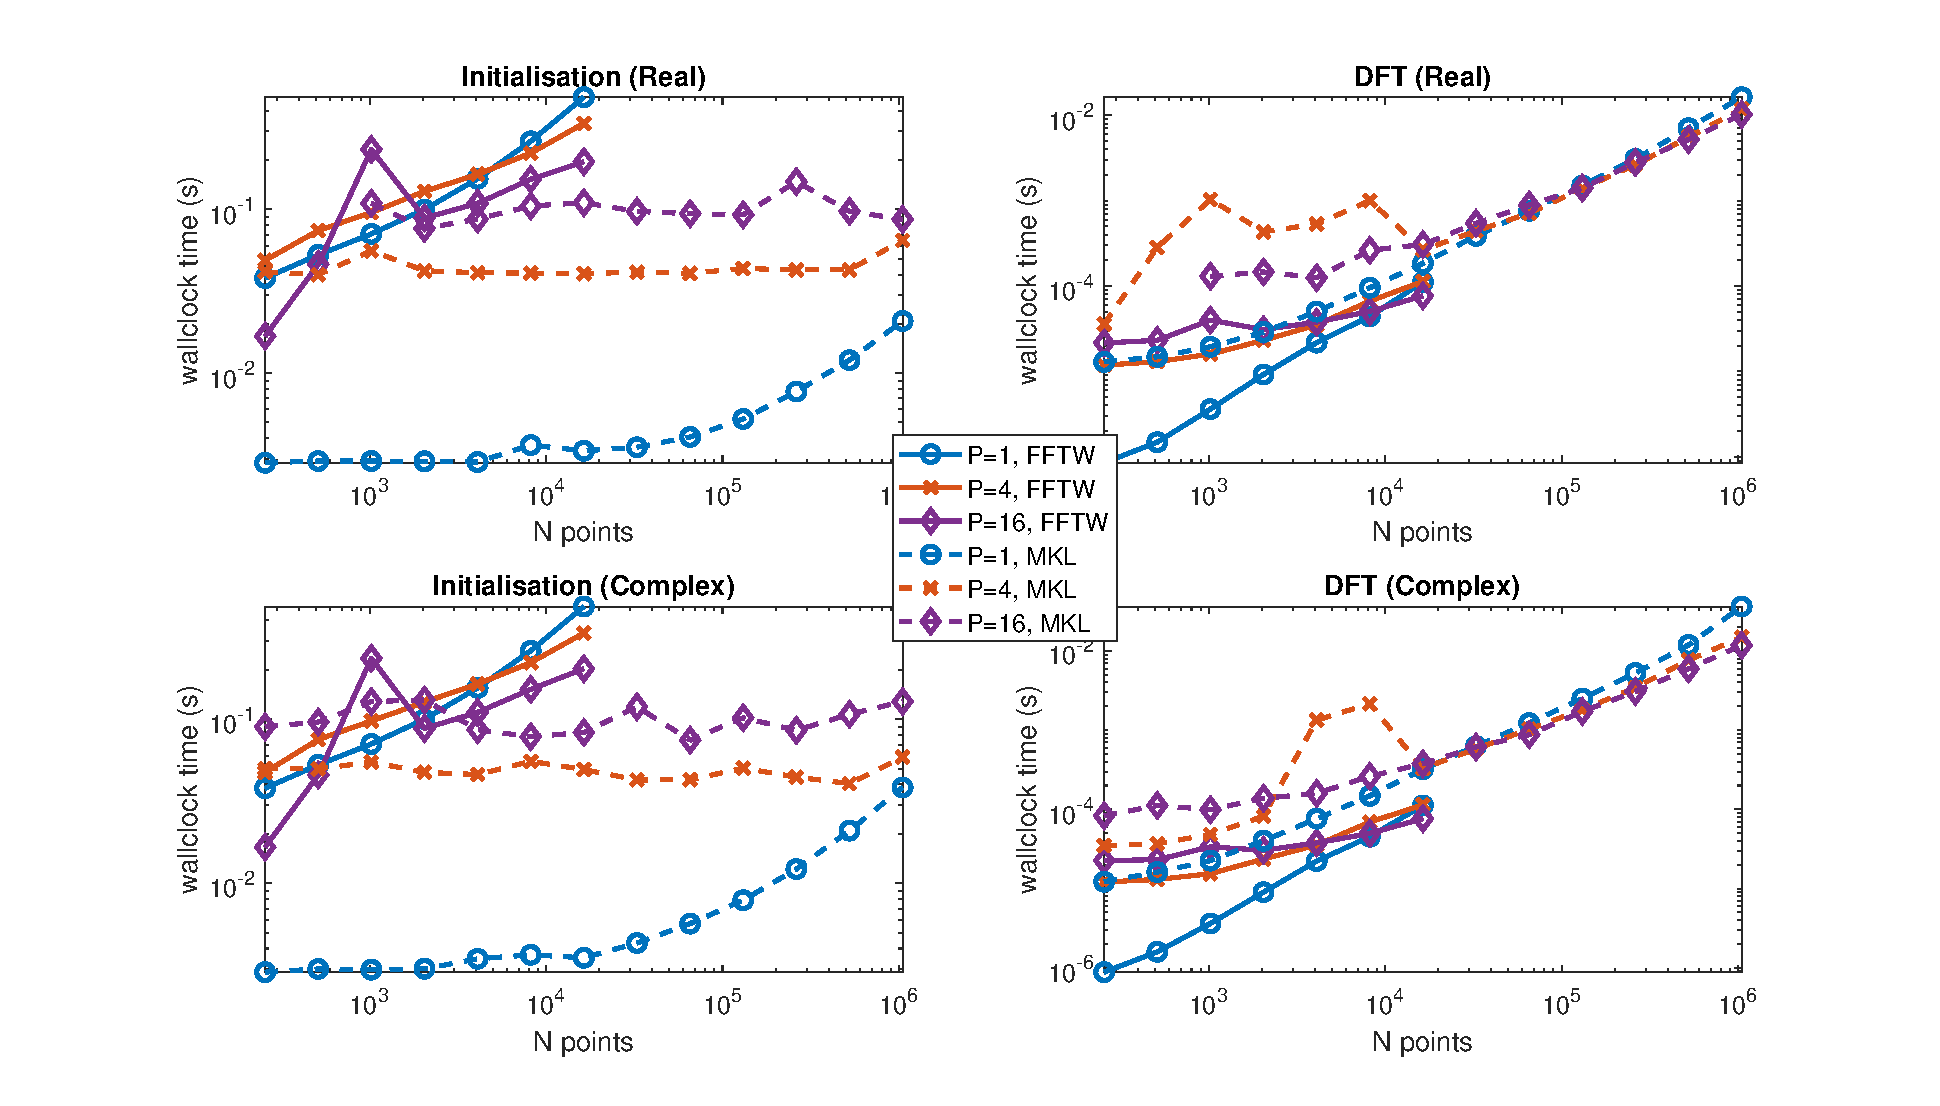
\includegraphics[width=\linewidth]{../results/fftw_mkl_2_1d_mpi.eps}
  \caption{Initialisation and DFT execution times of distributed FFTW and MKL libraries applied to 1D signal as a function of the
    number of points, $N,$ and varying the number of MPI processes, $P,$ with one thread per process. $N$ is a power of 2.}
  \label{1DDistFFTWMKL2}
\end{figure}


No prime comparison because MKL doesn't do prime N. Real values for FFTW were reals converted to complex values.


\section{Effect of domain size and distributed parallelisation for 2D benchmarks}\label{Sec:2DDistr}

\subsection{2D Distributed FFTW Library}\label{Sec:2DDistFFTW}

\begin{figure}[htb]
    \centering
    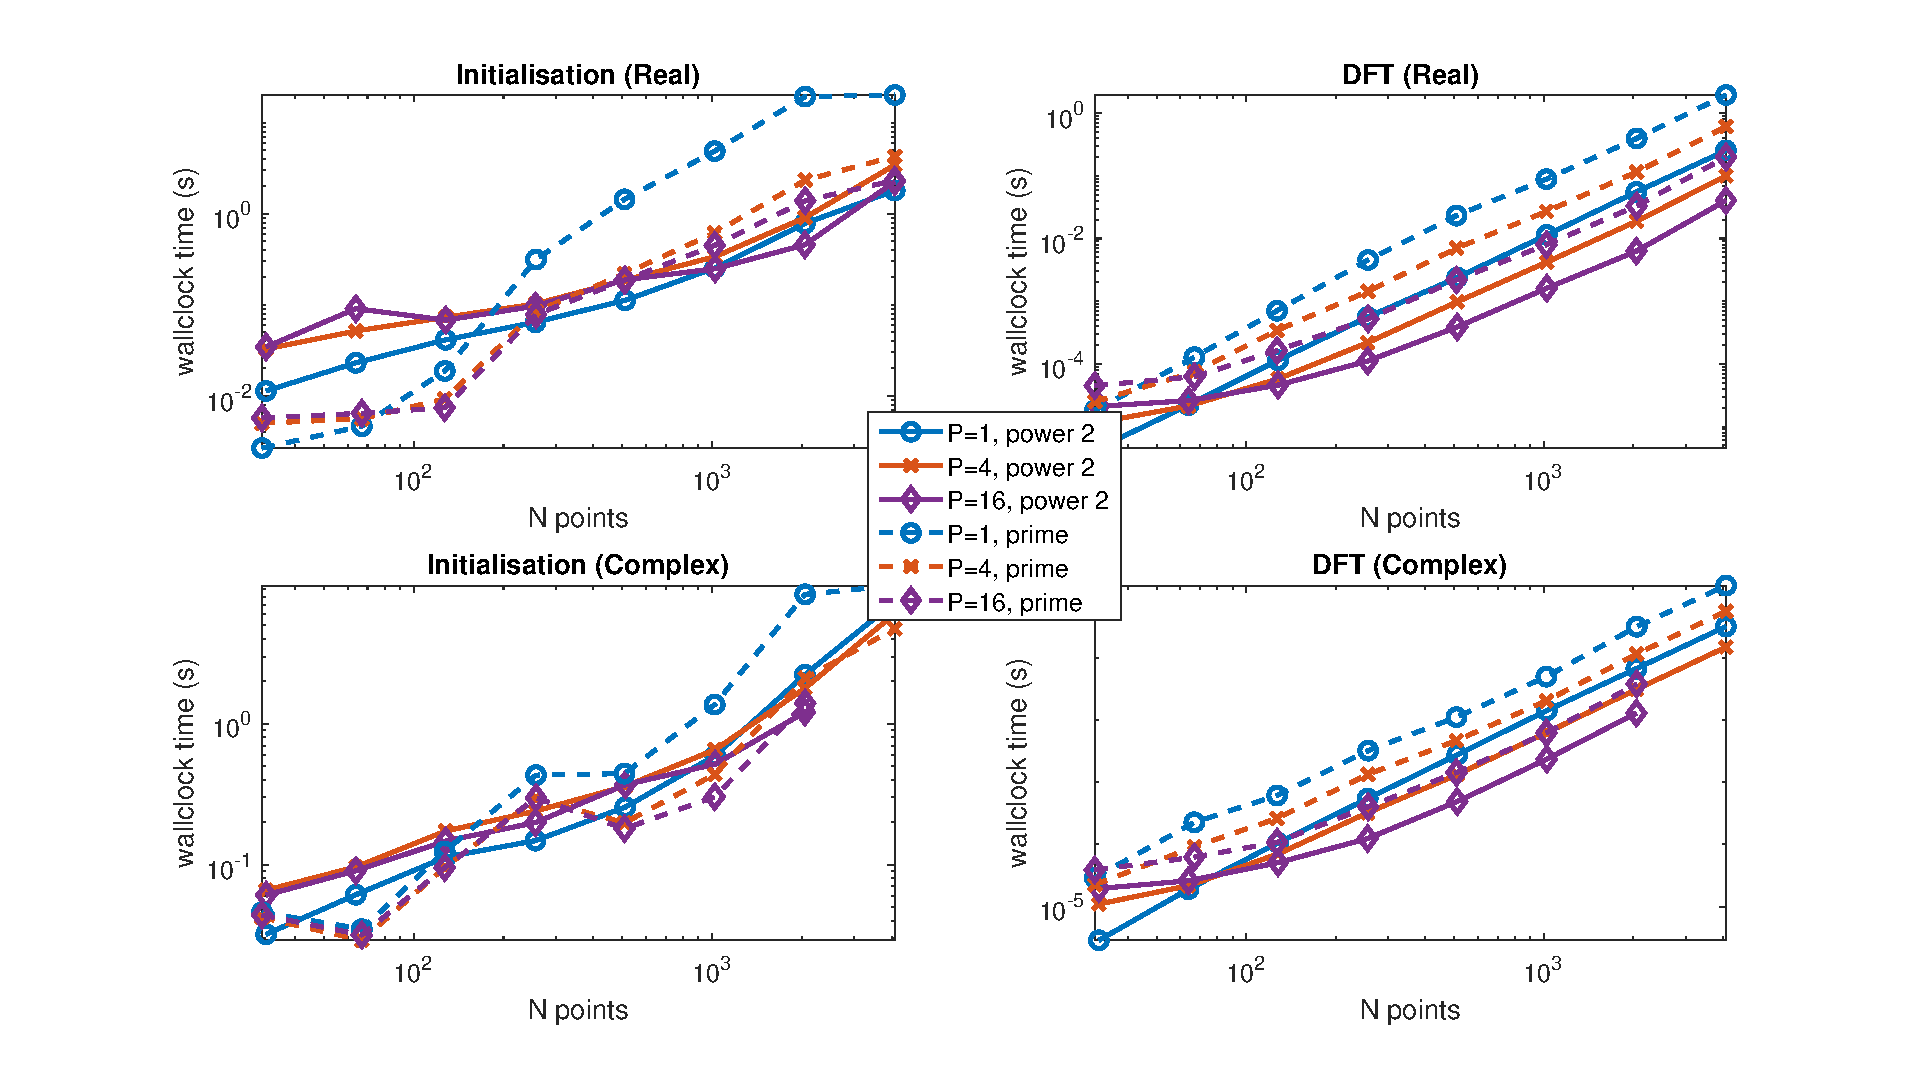
\includegraphics[width=\linewidth]{../results/fftw_2d_mpi.eps}
  \caption{Initialisation and DFT execution times of distributed FFTW library applied to 2D signal as a function of the
    number of points, $N,$ and varying the number of MPI processes, $P,$ with one thread per process.}
  \label{2DDistFFTW}
\end{figure}

\begin{figure}[htb]
    \centering
    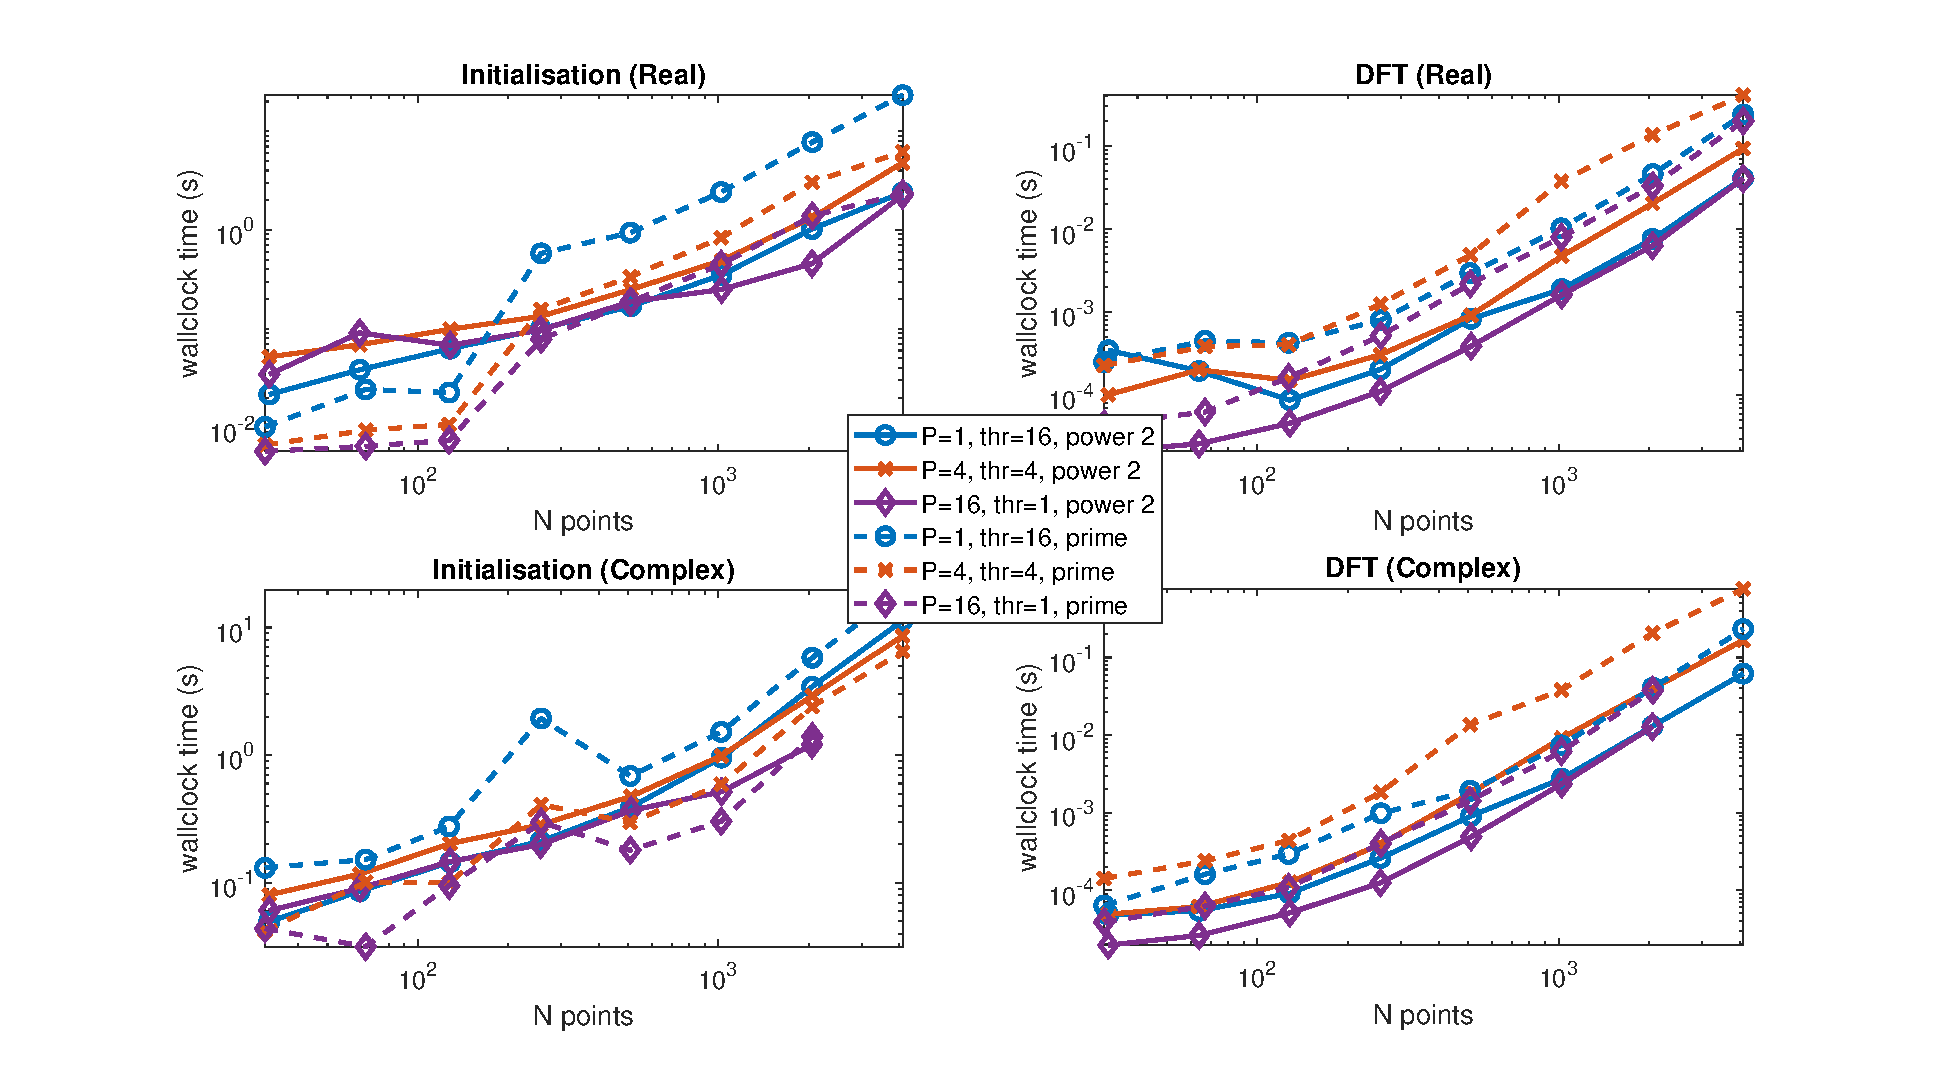
\includegraphics[width=\linewidth]{../results/fftw_2d_mpi_thr.eps}
  \caption{Initialisation and DFT execution times of distributed FFTW library applied to 2D signal as a function of the
    number of points, $N,$ and varying the number of MPI processes, $P,$ and threads, $thr,$ whilst maintaining $P\times thr=16.$}
  \label{2DDistFFTW16}
\end{figure}



\subsection{2D Distributed MKL Library}\label{Sec:2DDistMKL}

\begin{figure}[htb]
    \centering
    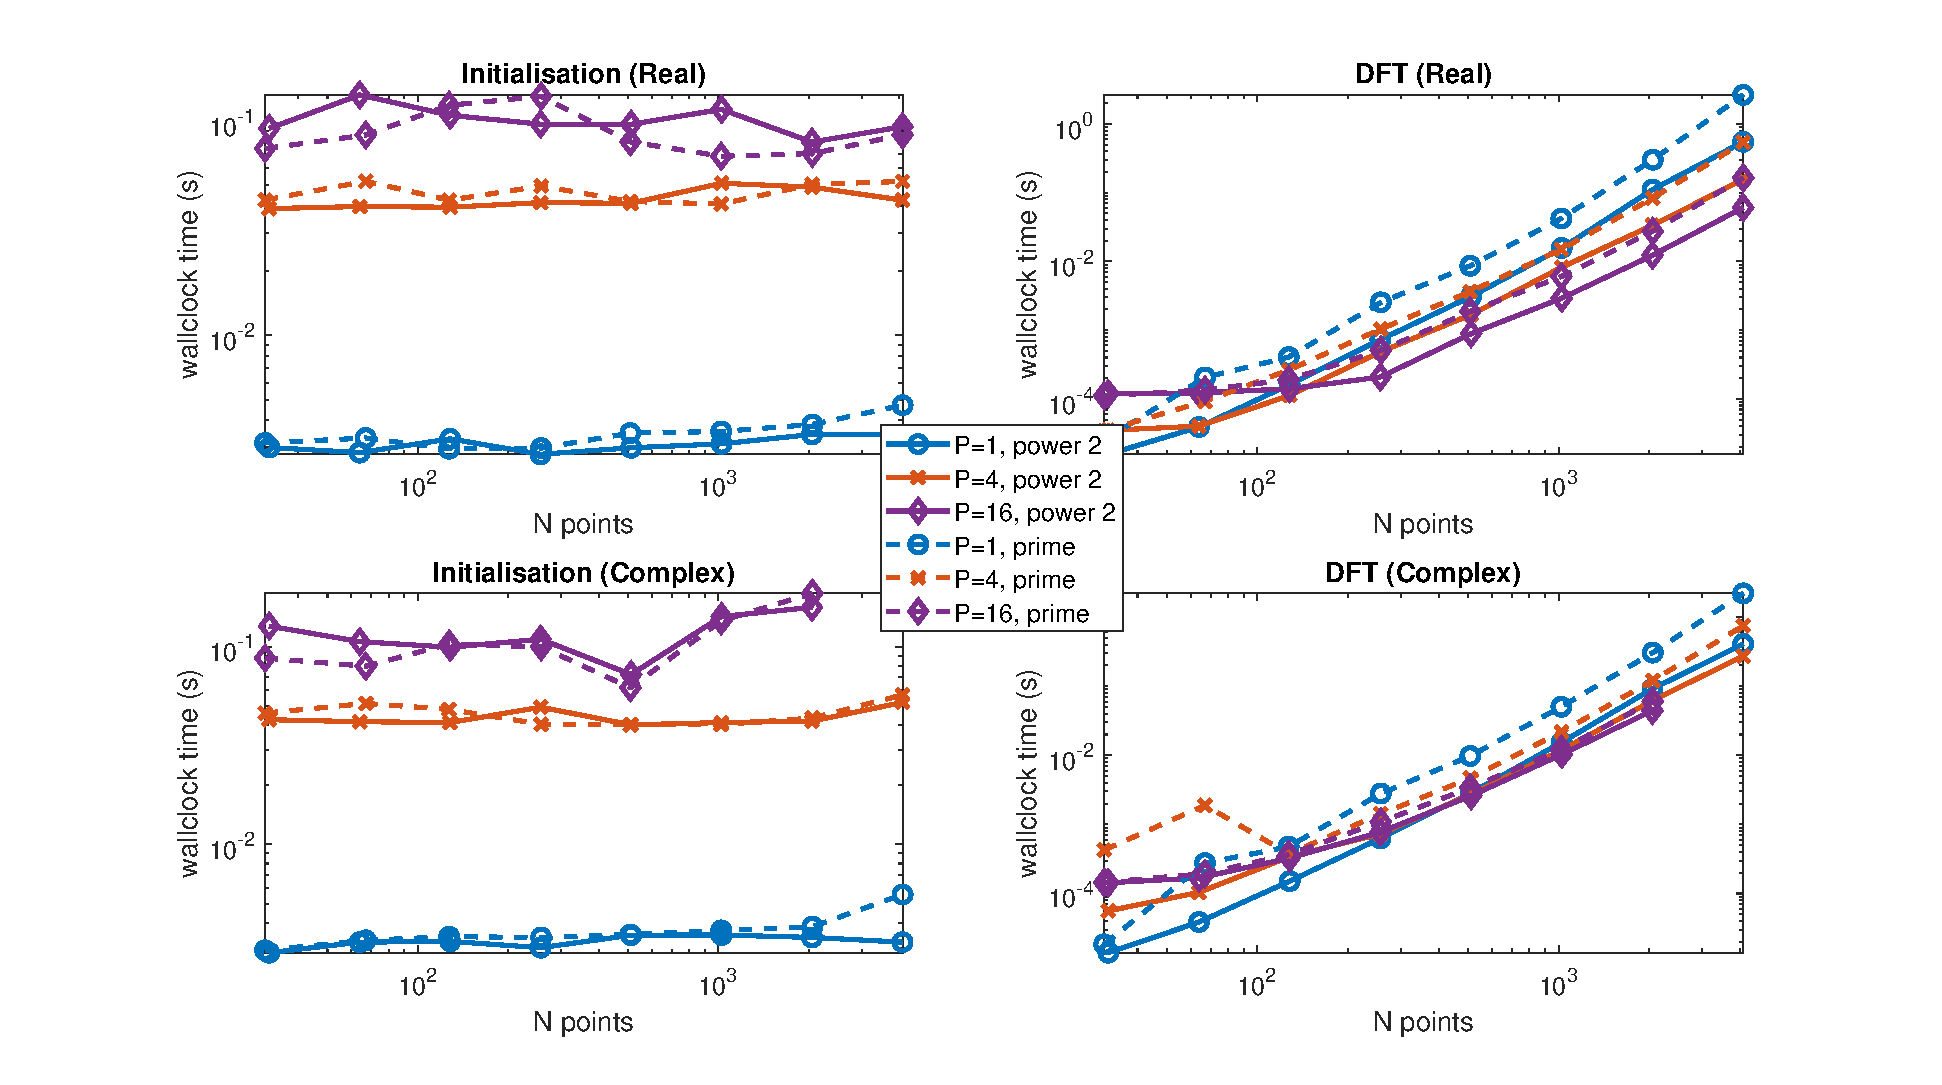
\includegraphics[width=\linewidth]{../results/mkl_2d_mpi.eps}
  \caption{Initialisation and DFT execution times of distributed MKL library applied to 2D signal as a function of the
    number of points, $N,$ and varying the number of MPI processes, $P,$ with one thread per process.}
  \label{2DDistMKL}
\end{figure}

\begin{figure}[htb]
    \centering
    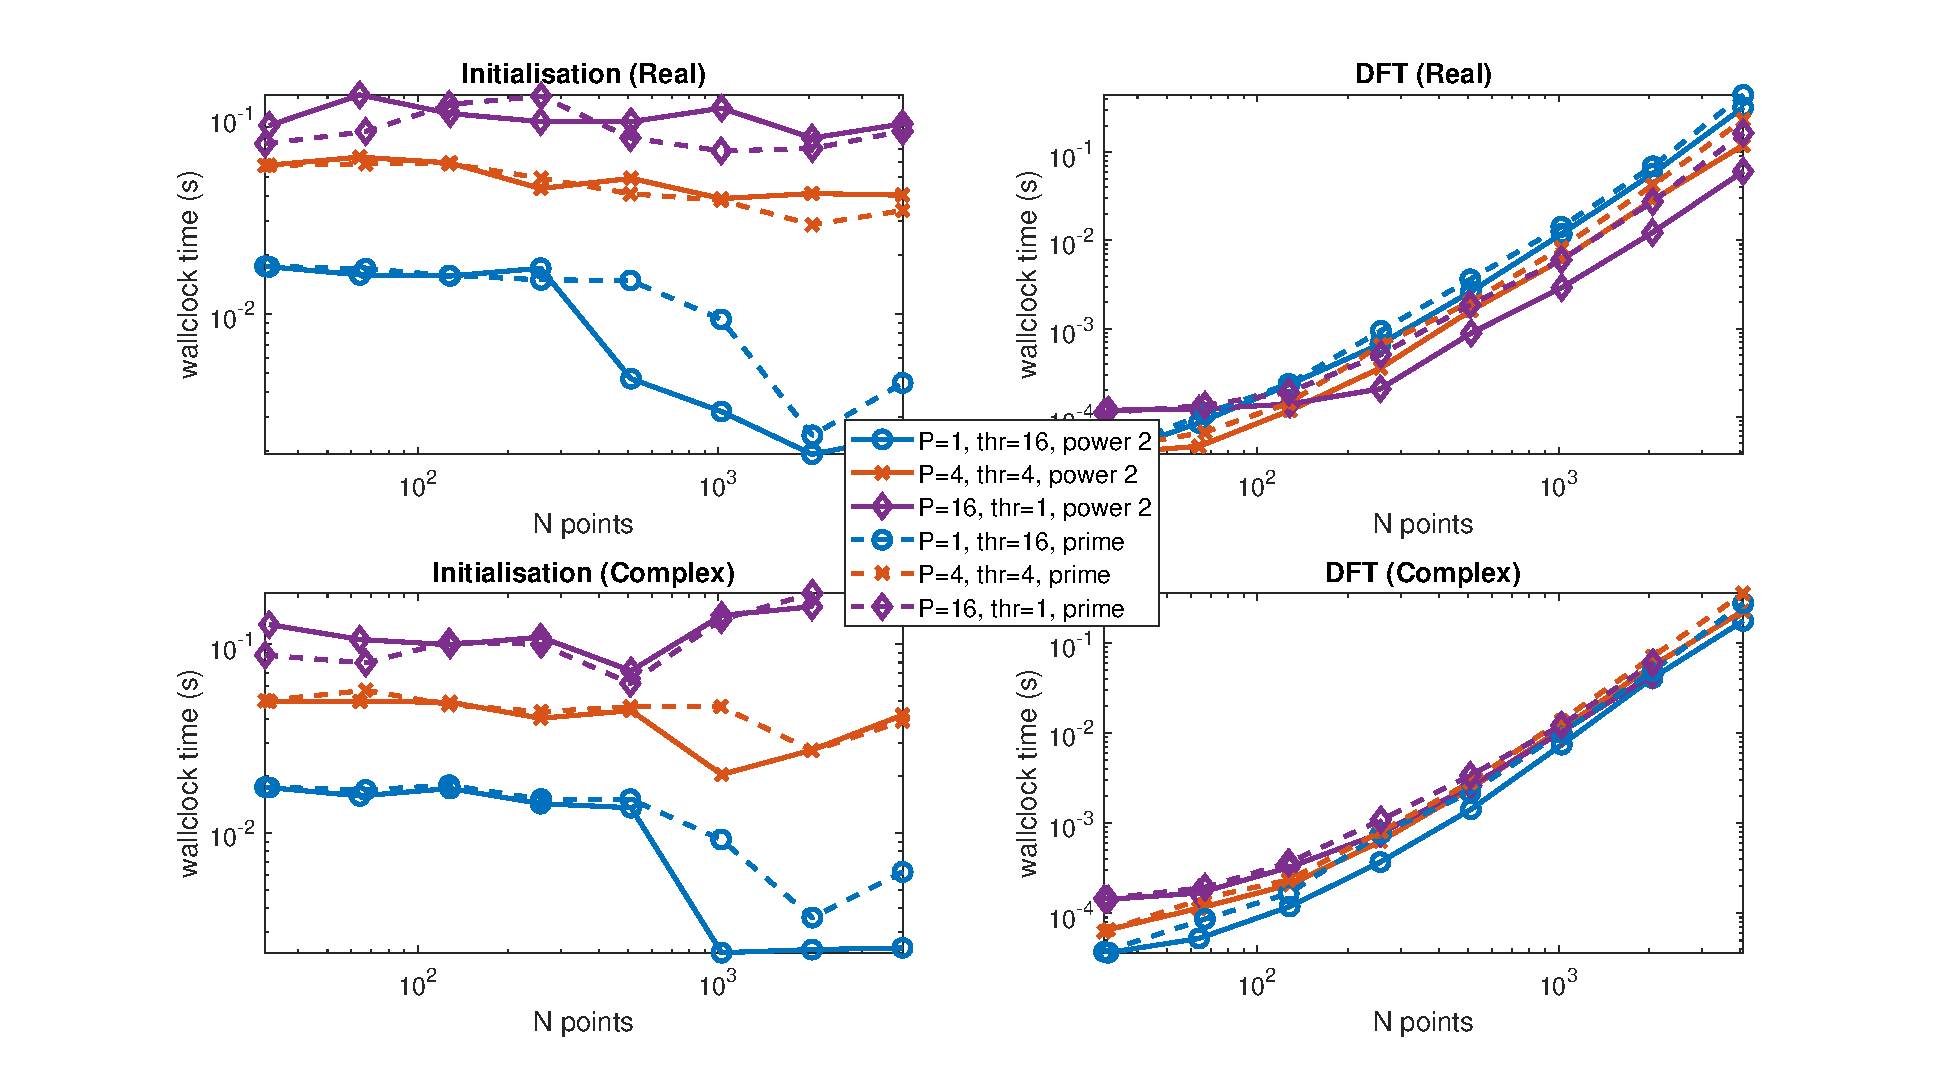
\includegraphics[width=\linewidth]{../results/mkl_2d_mpi_thr.eps}
  \caption{Initialisation and DFT execution times of distributed MKL library applied to 2D signal as a function of the
    number of points, $N,$ and varying the number of MPI processes, $P,$ and threads, $thr,$ whilst maintaining $P\times thr=16.$}
  \label{2DDistMKL16}
\end{figure}

\subsection{Comparison of distributed libraries for 2D benchmark}\label{Sec:2DDistComp}


\begin{figure}[htb]
    \centering
    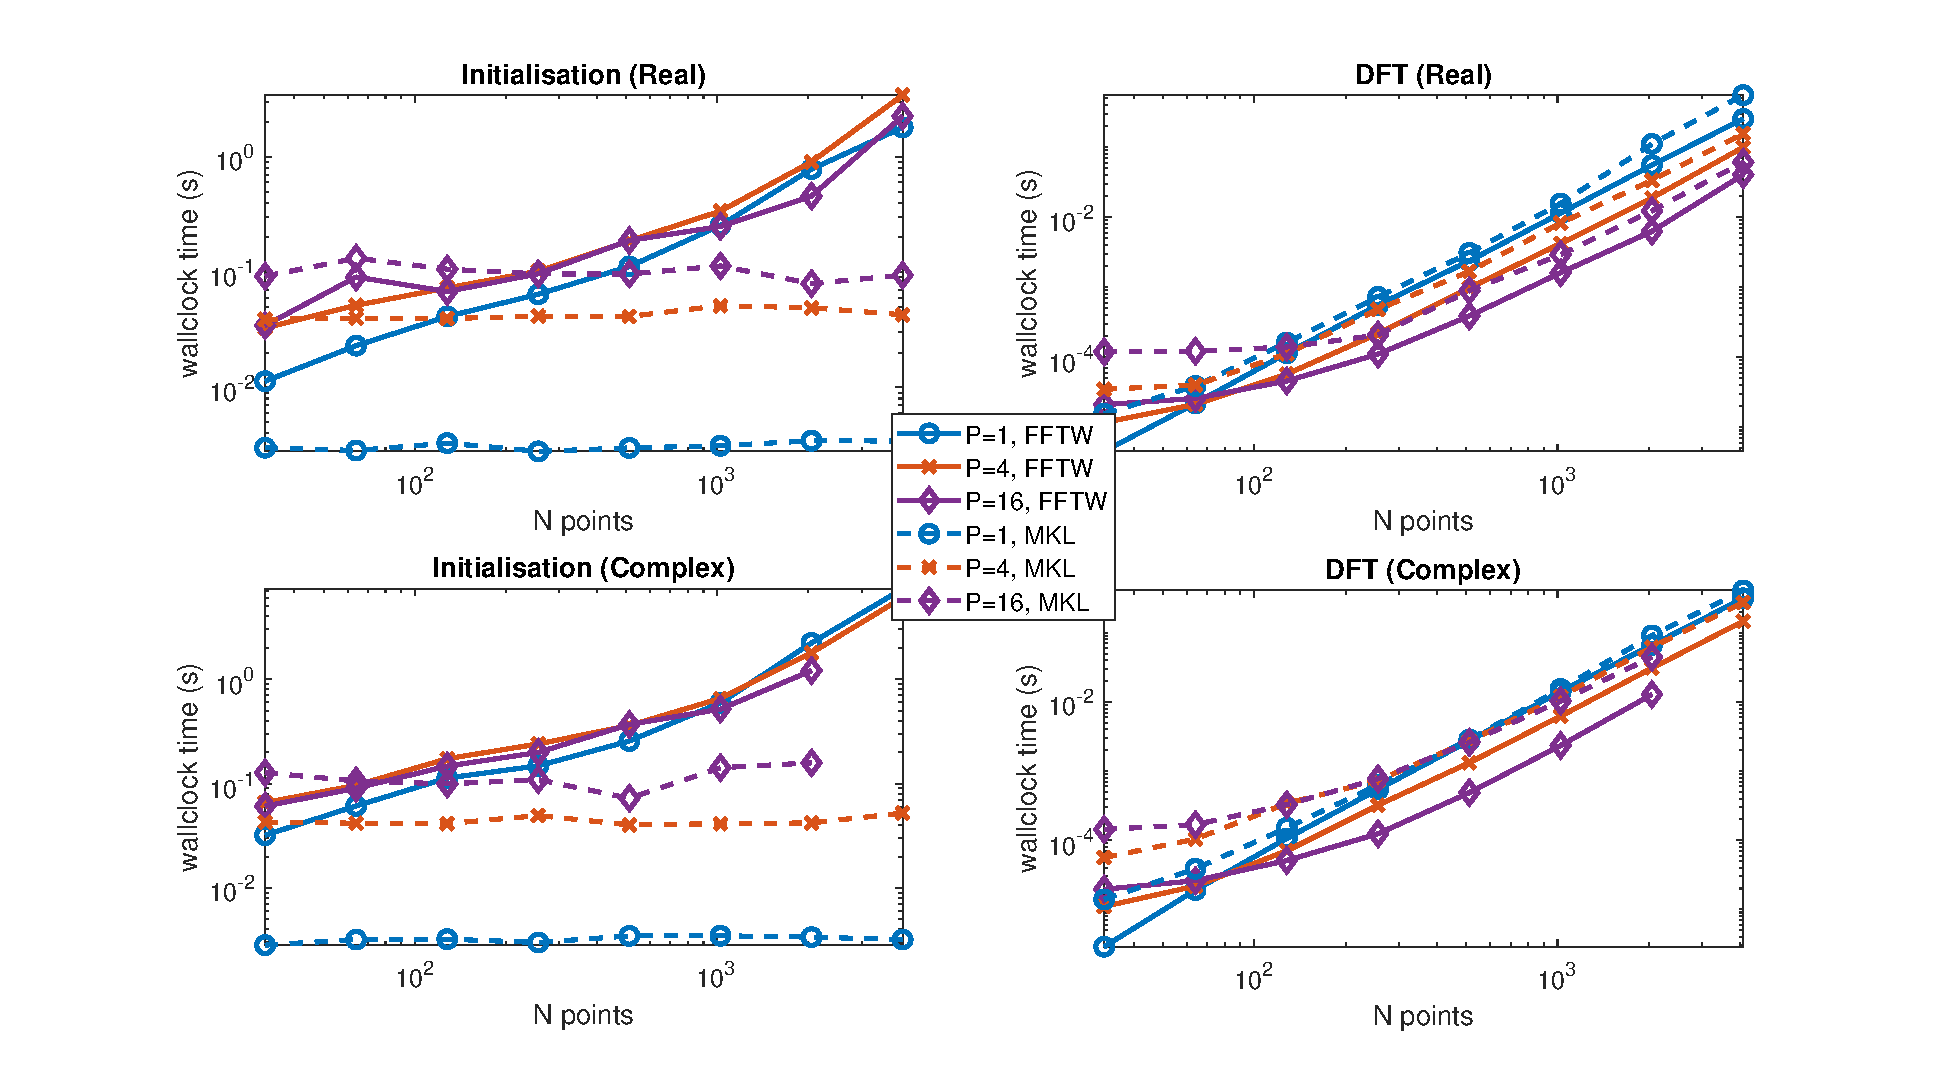
\includegraphics[width=\linewidth]{../results/fftw_mkl_2_2d_mpi.eps}
  \caption{Initialisation and DFT execution times of distributed FFTW and MKL libraries applied to 2D signal as a function of the
    number of points, $N,$ and varying the number of MPI processes, $P,$ with one thread per process. $N$ is a power of 2.}
  \label{2DDistFFTWMKL2}
\end{figure}


\begin{figure}[htb]
    \centering
    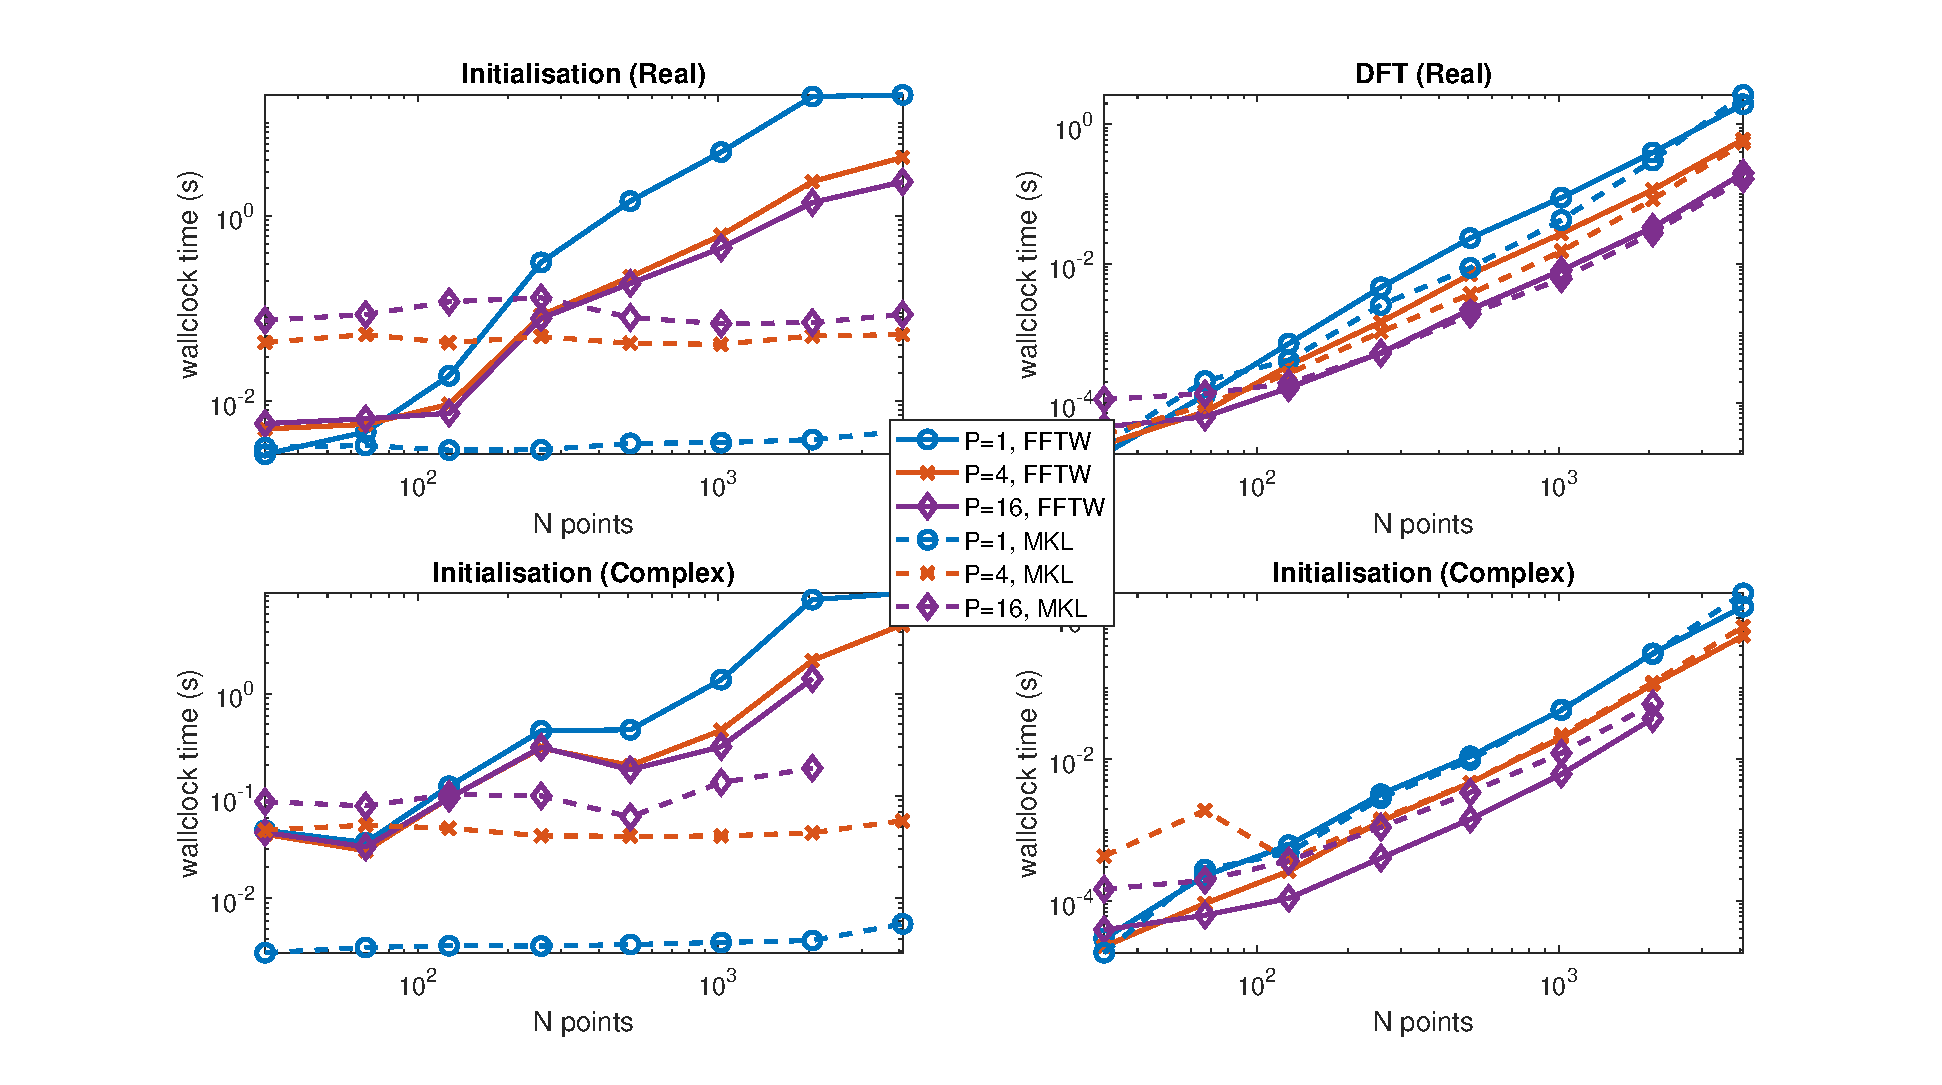
\includegraphics[width=\linewidth]{../results/fftw_mkl_prime_2d_mpi.eps}
  \caption{Initialisation and DFT execution times of distributed FFTW and MKL libraries applied to 2D signal as a function of the
    number of points, $N,$ and varying the number of MPI processes, $P,$ with one thread per process. $N$ is a prime number.}
  \label{2DDistFFTWMKLprime}
\end{figure}



\section{Effect of domain size and distributed parallelisation for 3D benchmarks}\label{Sec:3DDistr}

\subsection{3D Distributed FFTW Library}\label{Sec:3DDistFFTW}

\begin{figure}[htb]
    \centering
    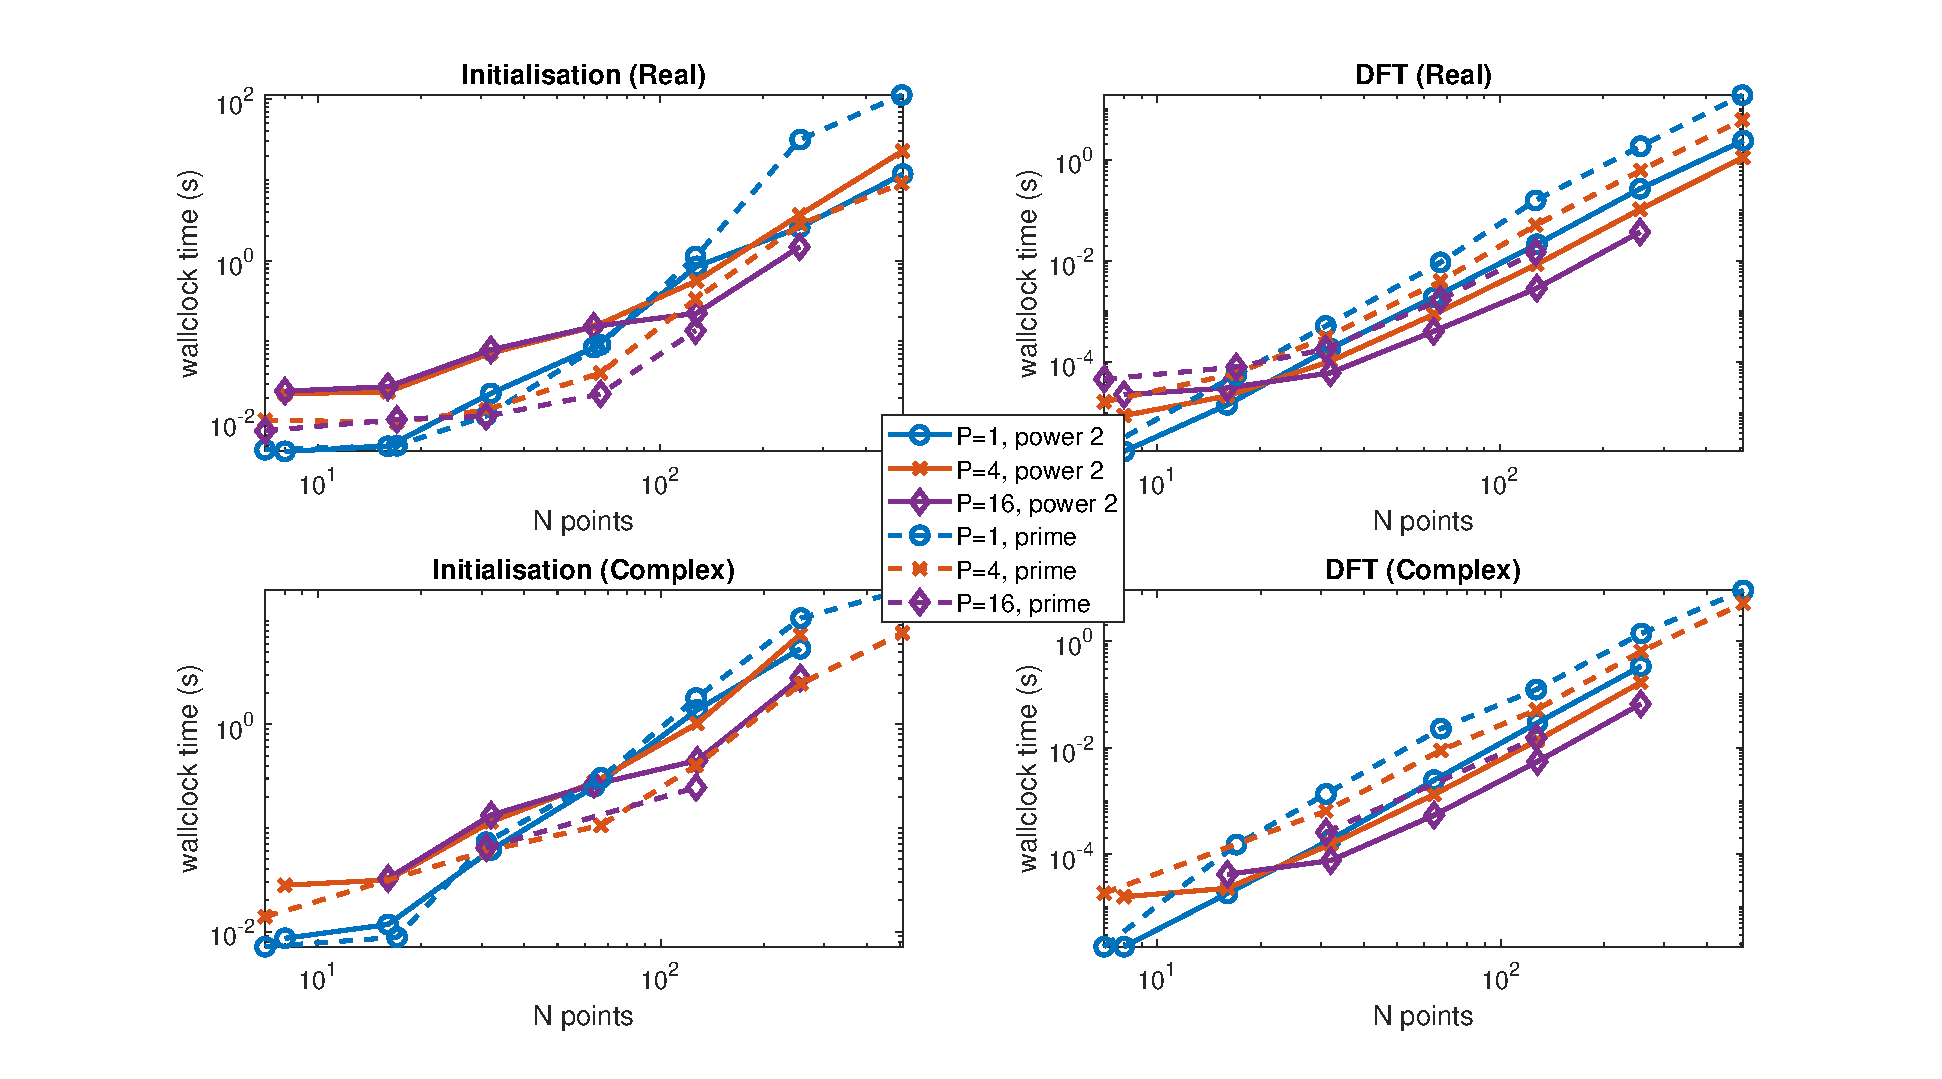
\includegraphics[width=\linewidth]{../results/fftw_3d_mpi.eps}
  \caption{Initialisation and DFT execution times of distributed FFTW library applied to 3D signal as a function of the
    number of points, $N,$ and varying the number of MPI processes, $P,$ with one thread per process.}
  \label{3DDistFFTW}
\end{figure}

\begin{figure}[htb]
    \centering
    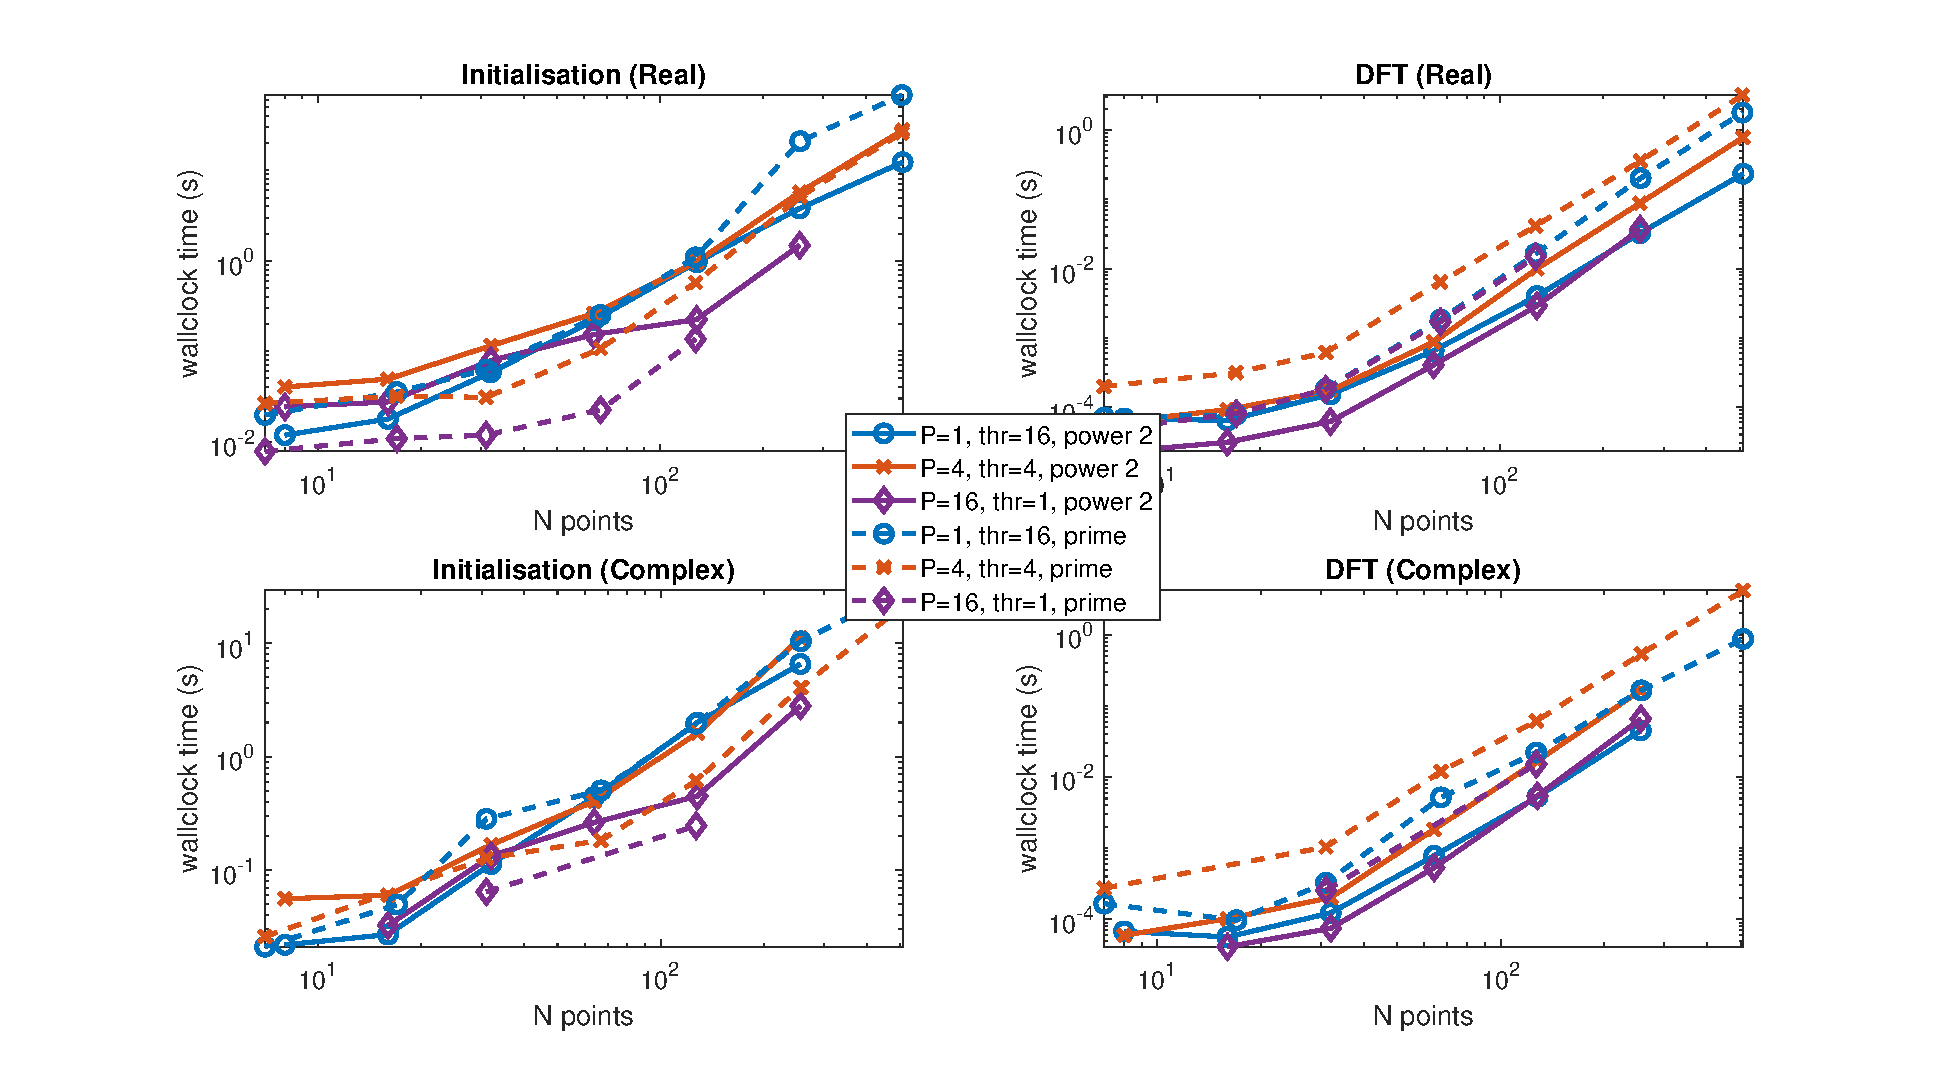
\includegraphics[width=\linewidth]{../results/fftw_3d_mpi_thr.eps}
  \caption{Initialisation and DFT execution times of distributed FFTW library applied to 3D signal as a function of the
    number of points, $N,$ and varying the number of MPI processes, $P,$ and threads, $thr,$ whilst maintaining $P\times thr=16.$}
  \label{3DDistFFTW16}
\end{figure}



\subsection{3D Distributed MKL Library}\label{Sec:3DDistMKL}

\begin{figure}[htb]
    \centering
    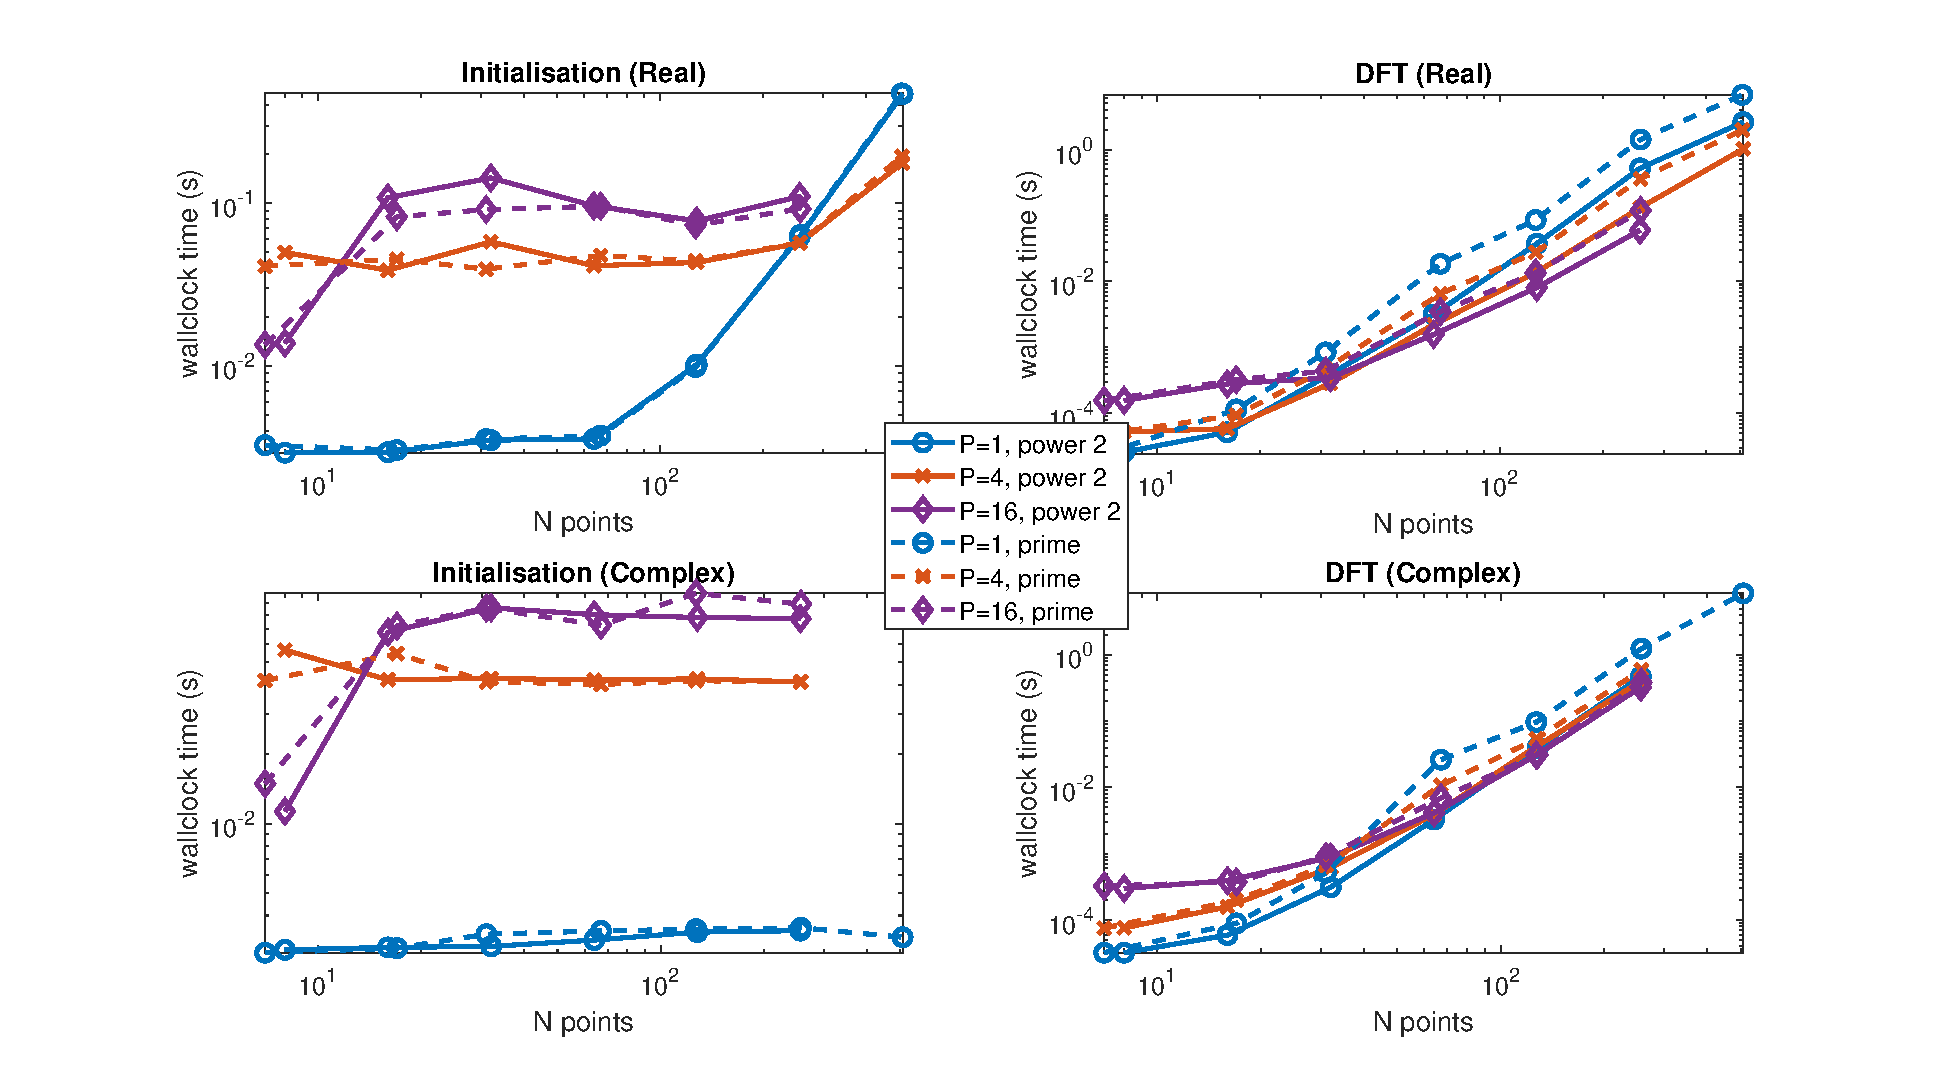
\includegraphics[width=\linewidth]{../results/mkl_3d_mpi.eps}
  \caption{Initialisation and DFT execution times of distributed MKL library applied to 3D signal as a function of the
    number of points, $N,$ and varying the number of MPI processes, $P,$ with one thread per process.}
  \label{3DDistMKL}
\end{figure}

\begin{figure}[htb]
    \centering
    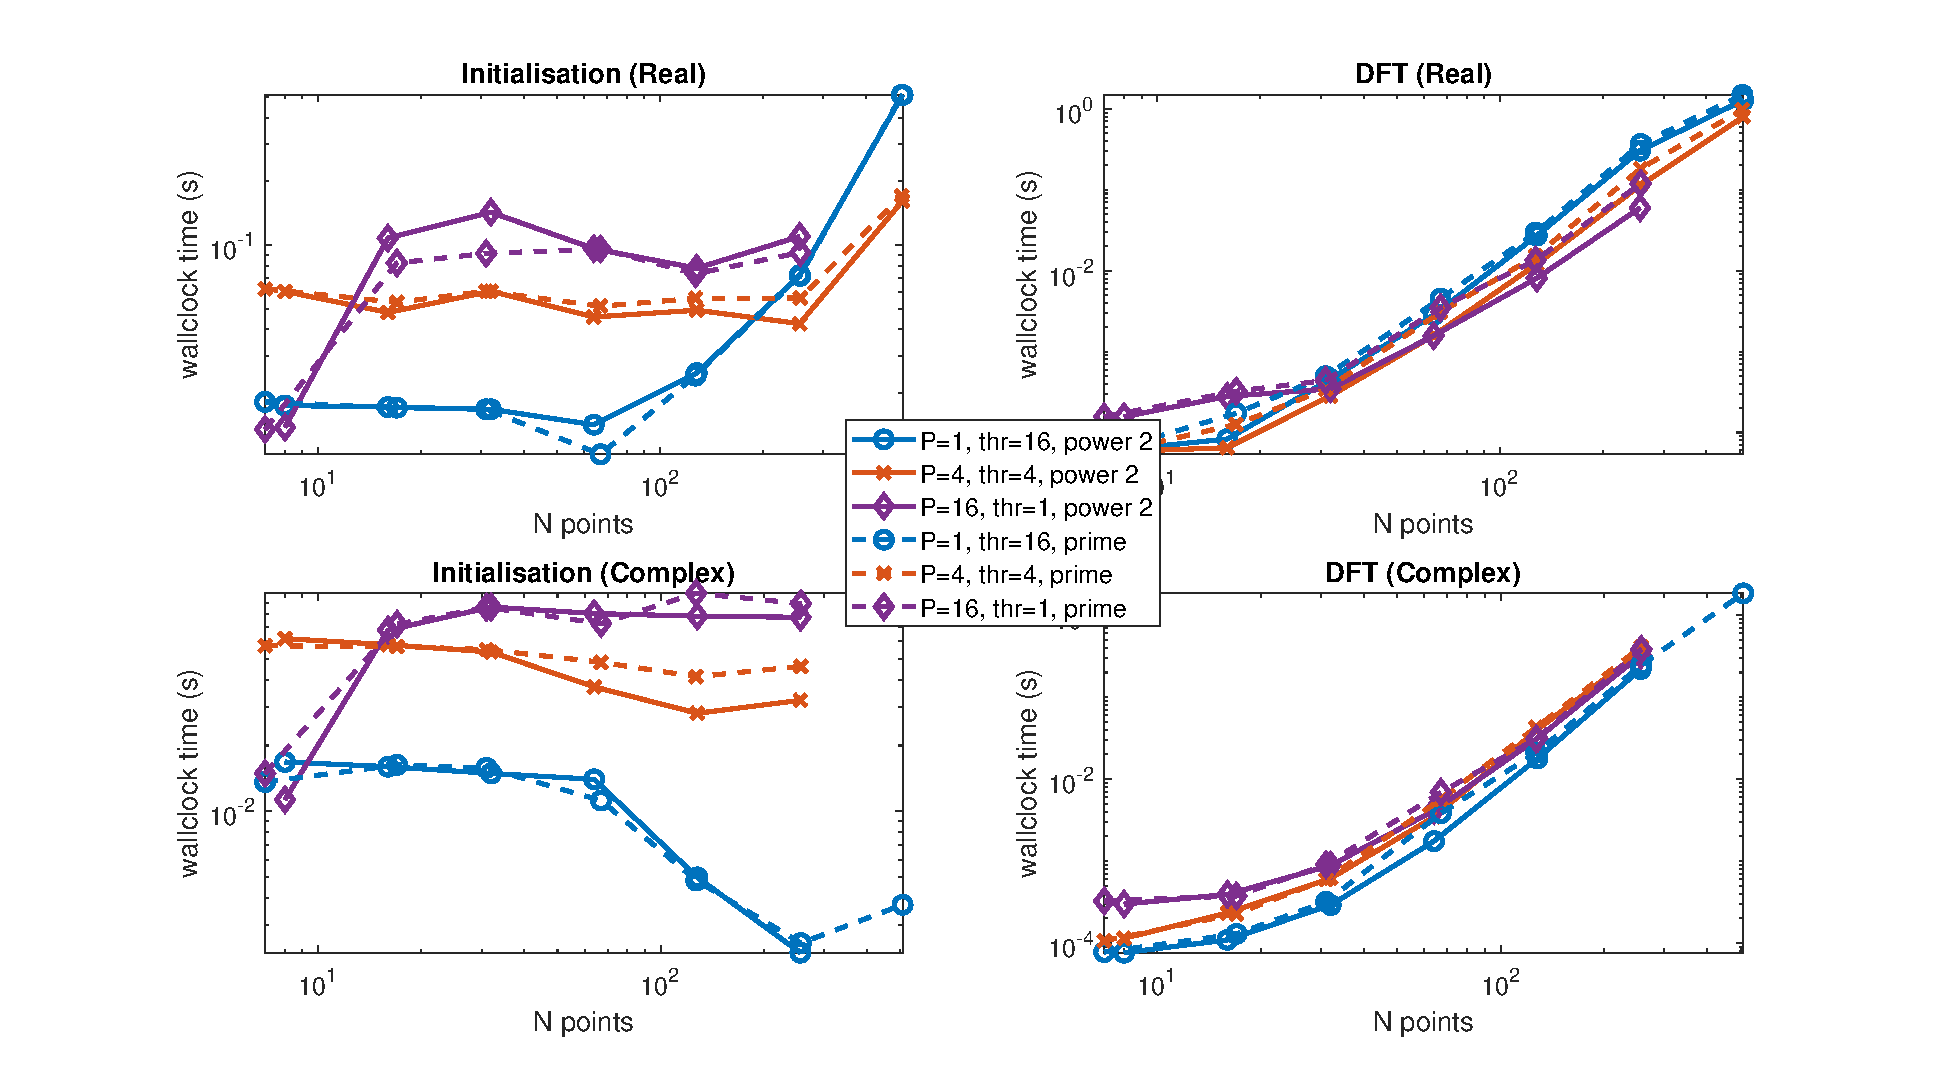
\includegraphics[width=\linewidth]{../results/mkl_3d_mpi_thr.eps}
  \caption{Initialisation and DFT execution times of distributed MKL library applied to 3D signal as a function of the
    number of points, $N,$ and varying the number of MPI processes, $P,$ and threads, $thr,$ whilst maintaining $P\times thr=16.$}
  \label{3DDistMKL16}
\end{figure}




\subsection{3D Distributed P3DFFT Library}\label{Sec:3DDistP3DFFT}

\begin{figure}[htb]
    \centering
    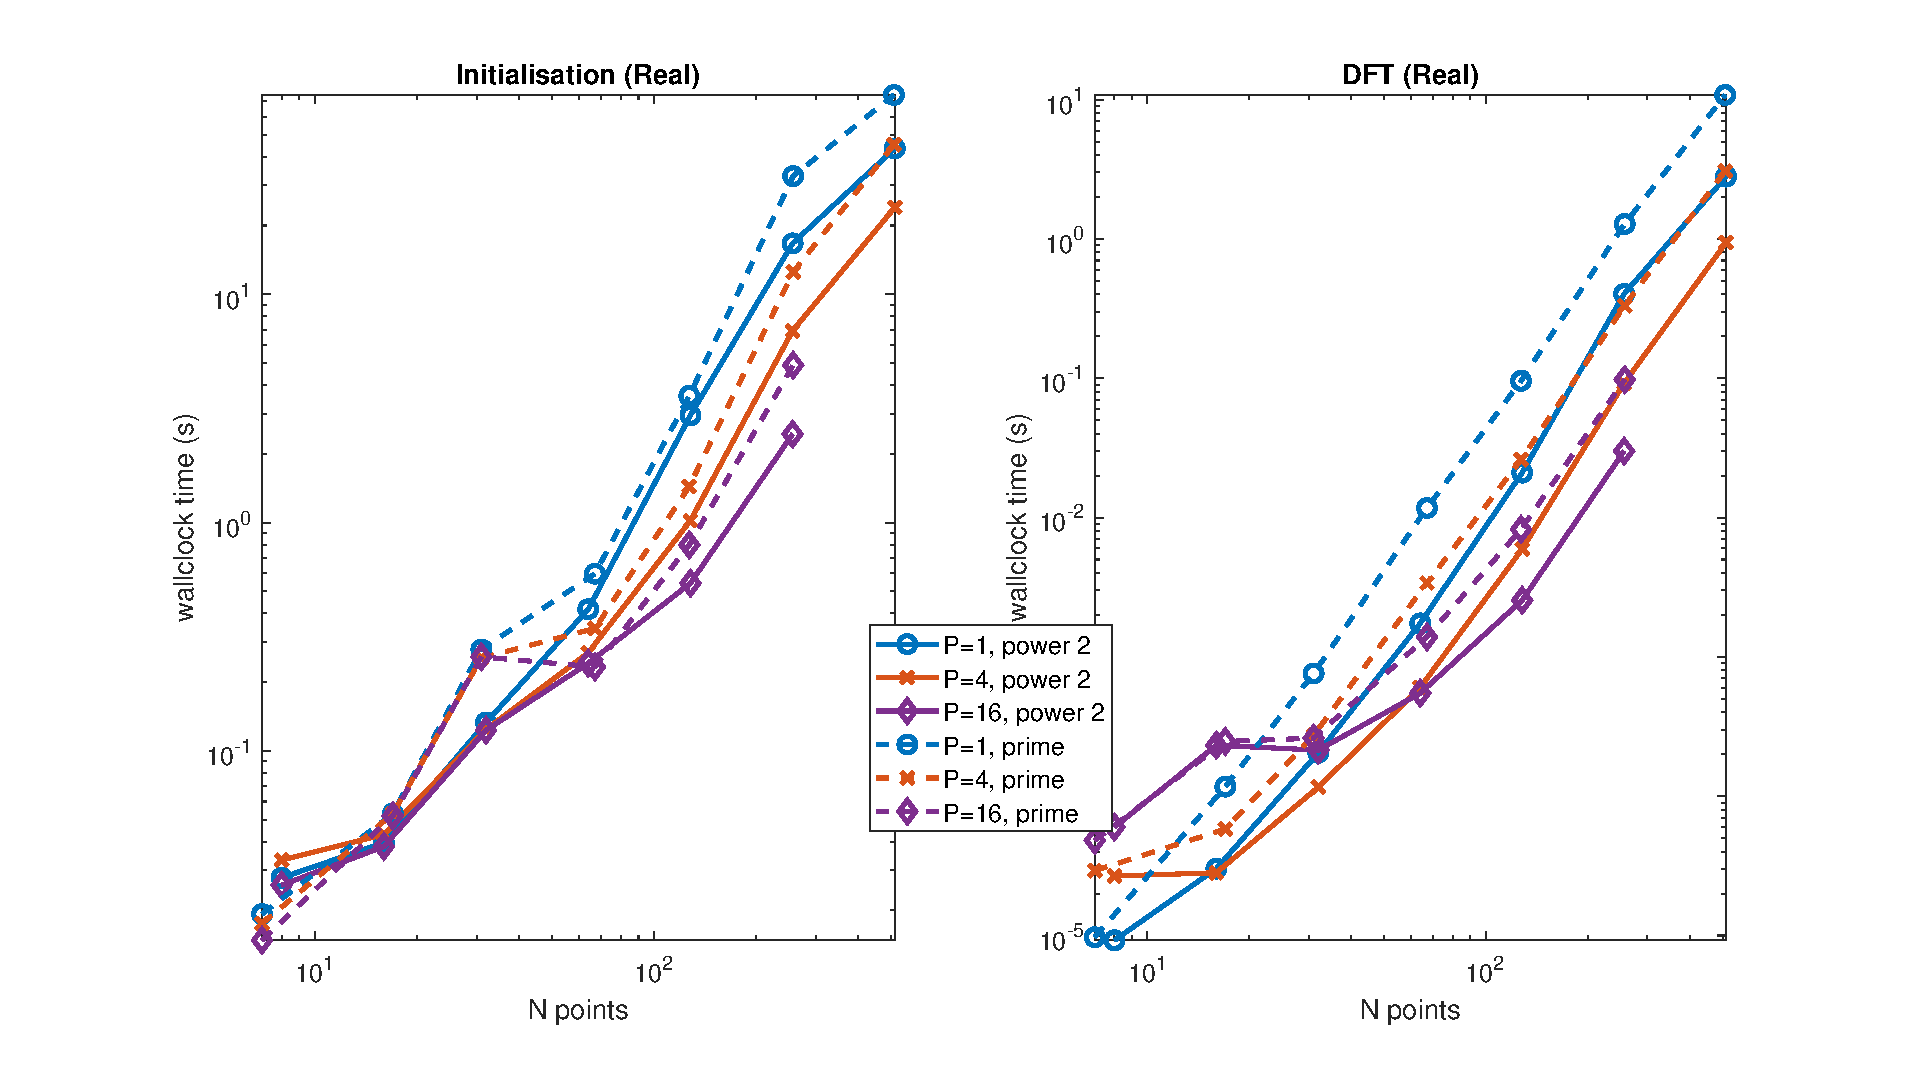
\includegraphics[width=\linewidth]{../results/p3dfft_3d_mpi.eps}
  \caption{Initialisation and DFT execution times of distributed P3DFFT library applied to 3D signal as a function of the
    number of points, $N,$ and varying the number of MPI processes, $P,$ with one thread per process.}
  \label{3DDistP3DFFT}
\end{figure}

\begin{figure}[htb]
    \centering
    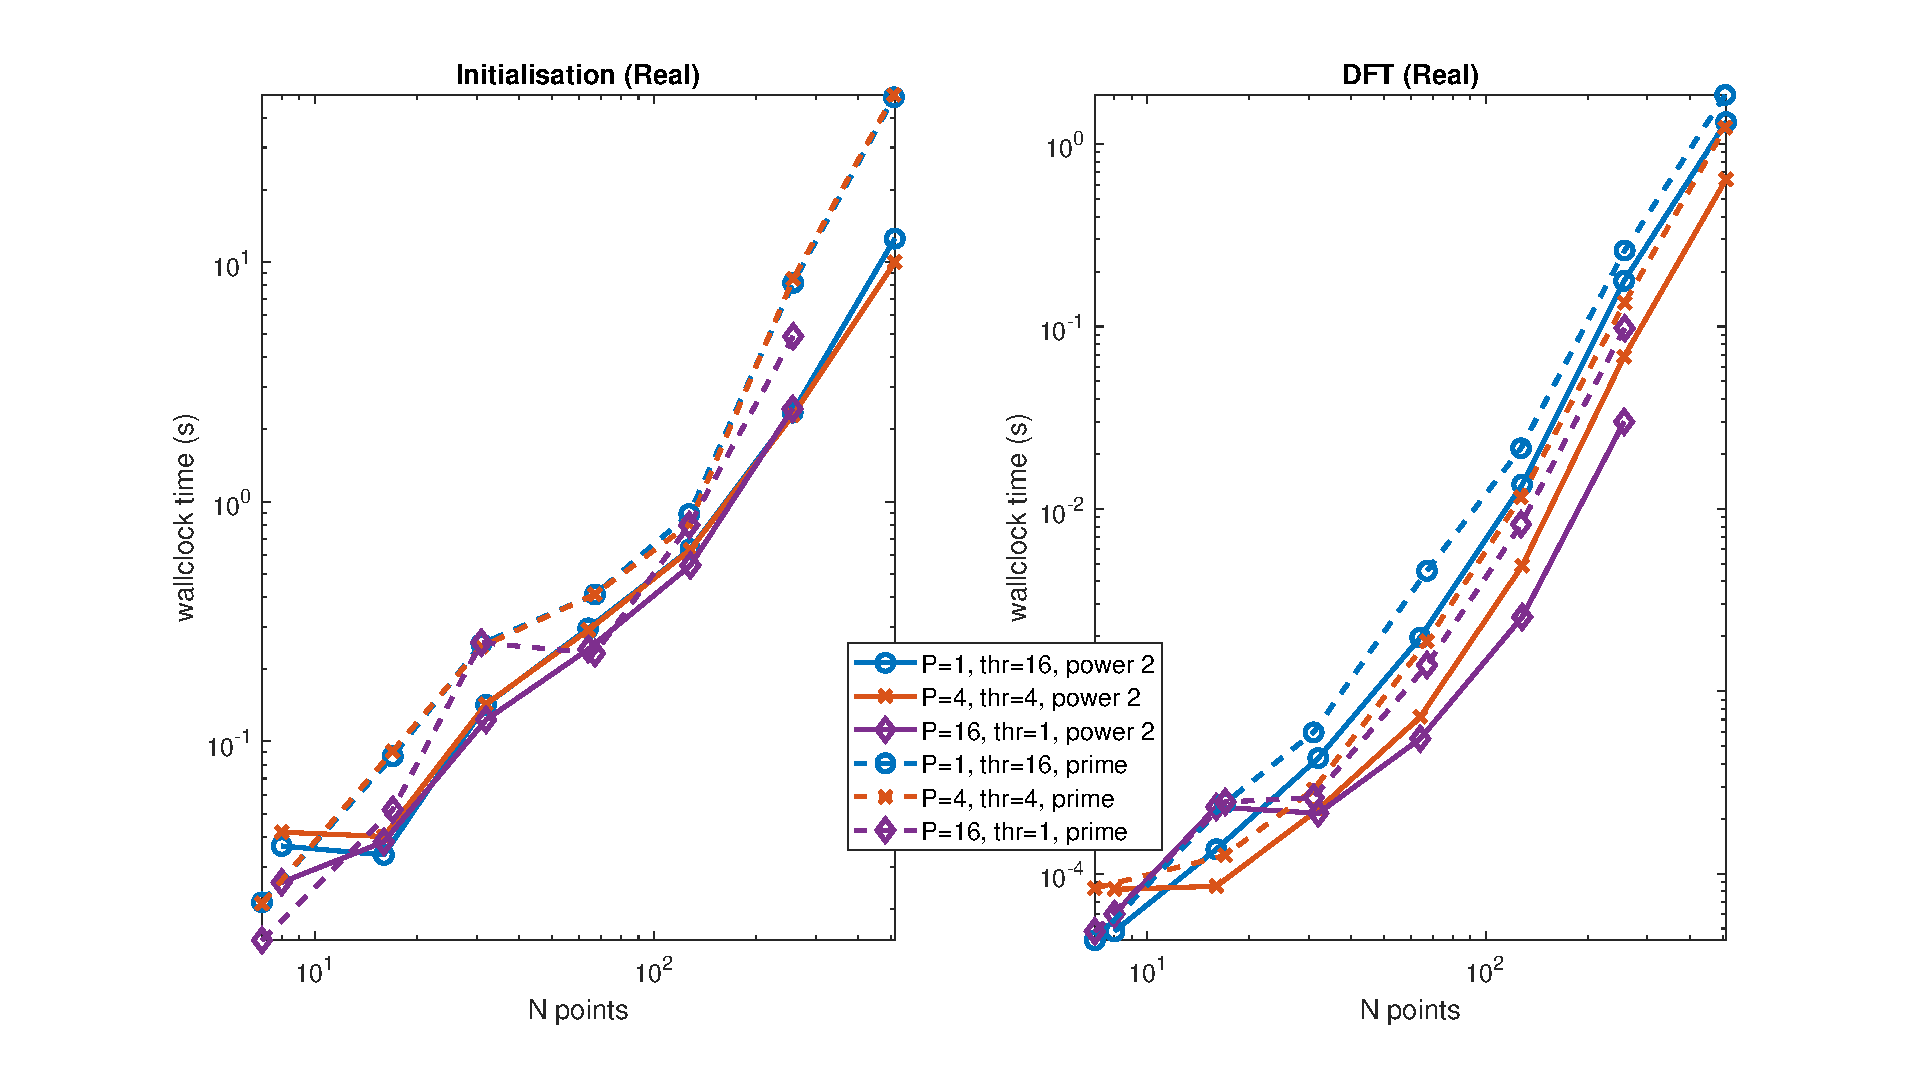
\includegraphics[width=\linewidth]{../results/p3dfft_3d_mpi_thr.eps}
  \caption{Initialisation and DFT execution times of distributed P3DFFT library applied to 3D signal as a function of the
    number of points, $N,$ and varying the number of MPI processes, $P,$ and threads, $thr,$ whilst maintaining $P\times thr=16.$}
  \label{3DDistP3DFFT16}
\end{figure}

\subsection{Comparison of distributed libraries for 3D benchmark}\label{Sec:3DDistComp}


\begin{figure}[htb]
    \centering
    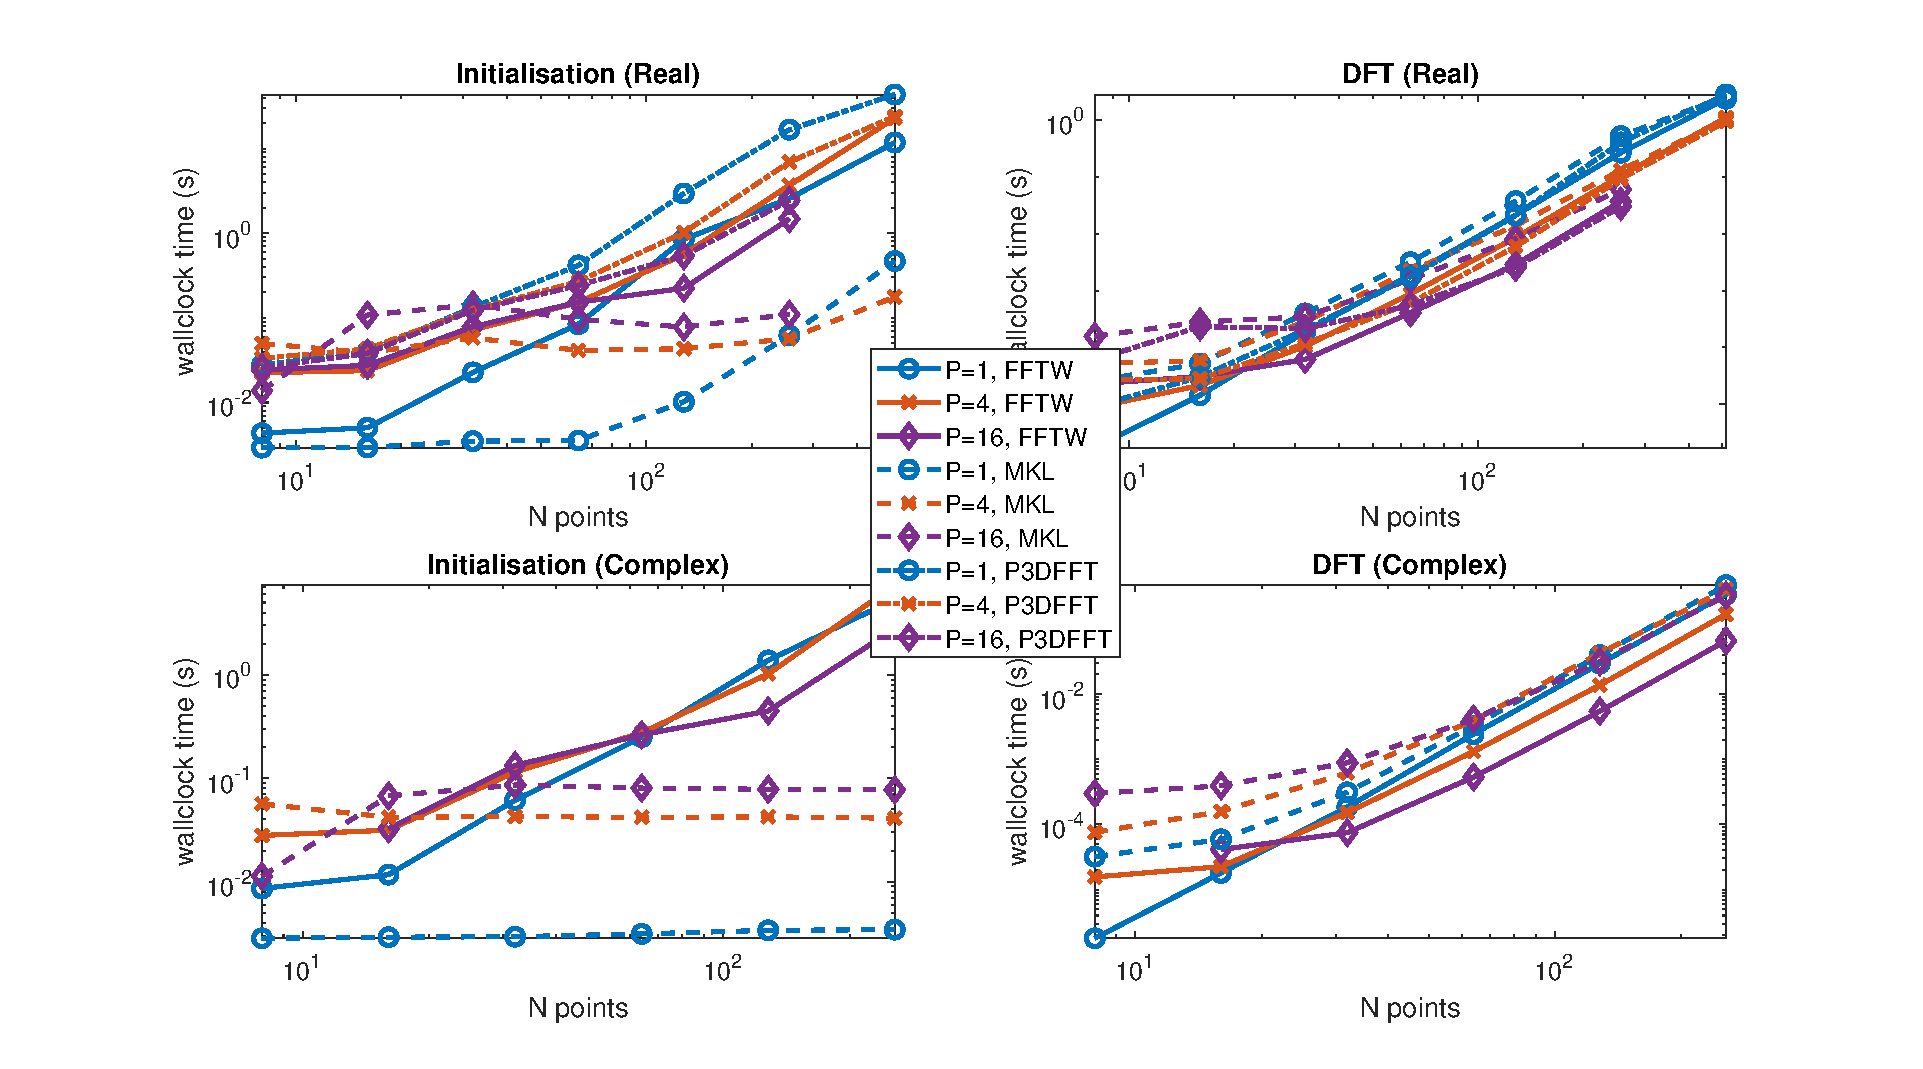
\includegraphics[width=\linewidth]{../results/fftw_mkl_p3dfft_2_3d_mpi.eps}
  \caption{Initialisation and DFT execution times of distributed FFTW, MKL and P3DFFT libraries applied to 3D signal as a function of the
    number of points, $N,$ and varying the number of MPI processes, $P,$ with one thread per process. $N$ is a power of 2.}
  \label{3DDistFFTWMKLP3DFFT2}
\end{figure}


\begin{figure}[htb]
    \centering
    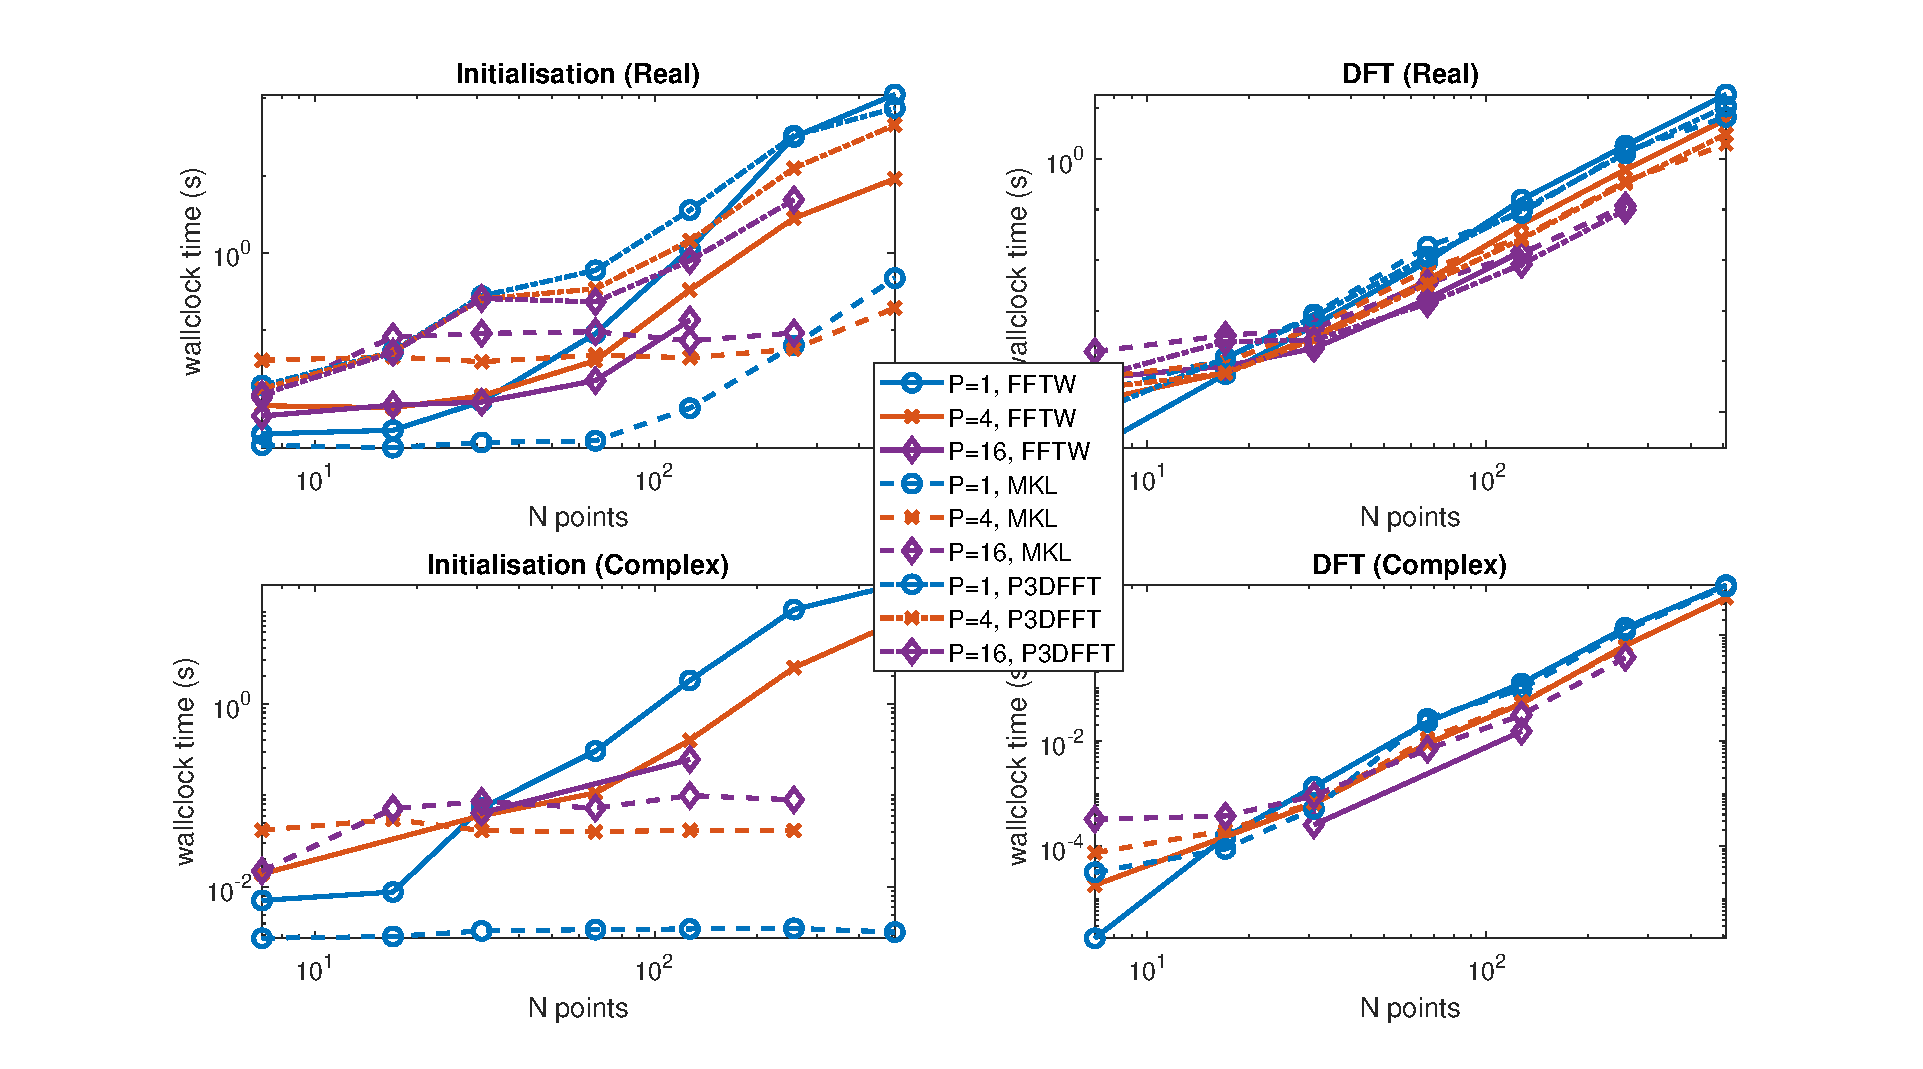
\includegraphics[width=\linewidth]{../results/fftw_mkl_p3dfft_prime_3d_mpi.eps}
  \caption{Initialisation and DFT execution times of distributed FFTW, MKL and P3DFFT libraries applied to 3D signal as a function of the
    number of points, $N,$ and varying the number of MPI processes, $P,$ with one thread per process. $N$ is a prime number.}
  \label{3DDistFFTWMKLP3DFFTprime}
\end{figure}



\section{Conclusions}\label{Sec:Conclusions}


\section*{Acknowledgements}
This work made use of computational support by CoSeC, the
Computational Science Centre for Research Communities, through its
Software Outlook activity.

\bibliographystyle{siam}
\bibliography{bib2017}

\clearpage

\appendix

\section{1D Multithreaded Data}\label{App:1Dthr}


\begin{table}[h]
\begin{center}
%\being{small}
\begin{tabular}{|r|r|r|r|r|r|r|r|r|r|}
\hline 
     \multicolumn{3}{|c|}{ } & \multicolumn{7}{c|}{$thr$} \\ \hline
    $N$  & & R/C  & 1           & 2    & 4    & 8    & 12   & 16    & 24  \\ \hline\hline
    2048  & ftime & R  &  1.09e-5 &   1.71e-5 &   3.00e-5 &   3.49e-5 &   4.05e-5 &   4.54e-5 &   6.26e-5   \\ 
      & fratio & & 1.00 &    1.57 &    2.75 &    3.20 &    3.72 &    4.17 &    5.74   \\ 
     & itime & &  8.13e-2 &    1.09e-1 &   1.18e-1 &   1.42e-1 &   1.72e-1 &   1.62e-1 &   2.14e-1    \\ 
     & iratio & &   1.00 &    1.34 &    1.45 &    1.75 &    2.12 &    1.99 &    2.63    \\ \hline 
    2053  & ftime & R &  1.03e-4 &   1.20e-4 &   1.73e-4 &   1.93e-4 &   2.50e-4 &   3.81e-4 &   7.14e-4    \\ 
      & fratio & & 1.00 &   1.17 &   1.68 &   1.87 &   2.43 &   3.70 &   6.93    \\ 
     & itime &  &   1.08e0 &   1.71e0 &   2.07e0 &   2.51e0 &   2.93e0 &   3.21e0 &   3.79e0   \\ 
    & iratio &  &     1.00 &   1.58 &   1.92 &   2.32 &   2.71 &   2.97 &   3.51     \\ \hline 
  16381  & ftime & R &  7.97e-4 &   7.98e-4 &   8.19e-4 &   8.25e-4 &   8.30e-4 &   8.47e-4 &   9.57e-4     \\ 
      & fratio & &  1.00 &   1.00 &   1.03 &   1.04 &   1.04 &   1.06 &   1.20    \\ 
     & itime & &  1.51e0 &   2.05e0 &   2.29e0 &   2.56e0 &   2.84e0 &   3.07e0 &   3.67e0     \\ 
     & iratio & &  1.00 &   1.36 &   1.52 &   1.70 &   1.88 &   2.03 &   2.43     \\ \hline 
 16384  & ftime & R & 1.11e-4 &   8.58e-5 &   9.49e-5 &   8.59e-5 &   9.79e-5 &   2.06e-4 &   5.42e-4   \\ 
      & fratio & & 1.00 &   0.77 &   0.85 &   0.77 &   0.88 &   1.86 &   4.88  \\
     & itime & & 1.90e-1 &   2.62e-1 &   2.55e-1 &   2.60e-1 &   3.07e-1 &   2.90e-1 &   3.98e-1   \\ 
 & iratio & & 1.00 &   1.38 &   1.34 &   1.37 &   1.62 &   1.53 &   2.09   \\  \hline \hline
    2048  & ftime & C  &  1.01e-5 &   1.84e-5 &   2.98e-5 &   3.39e-5 &   3.72e-5 &   4.94e-5 &   5.92e-5   \\ 
      & fratio & &  1.00 &   1.82 &   2.95 &   3.36 &   3.68 &   4.89 &   5.86  \\ 
     & itime & &   1.07e-1 &   1.16e-1 &   1.55e-1 &   1.80e-1 &   2.10e-1 &   2.12e-1 &   2.68e-1   \\ 
     & iratio & &  1.00 &   1.08 &   1.45 &   1.68 &   1.96 &   1.98 &   2.50     \\ \hline 
    2053  & ftime & C &  7.76e-5 &   1.03e-4 &   1.32e-4 &   1.81e-4 &   1.83e-4 &   2.30e-4 &   4.48e-4     \\ 
      & fratio & &  1.00 &   1.33 &   1.70 &   2.33 &   2.36 &   2.96 &   5.77   \\ 
     & itime &  &  1.03e0 &   1.06e0 &   1.24e0 &   1.47e0 &   1.74e0 &   1.89e0 &   2.21e0    \\ 
    & iratio &  &  1.00 &   1.03 &   1.20 &   1.43 &   1.69 &   1.84 &   2.15       \\ \hline
  16381  & ftime & C &   1.03e-3 &   6.76e-4 &   6.62e-4 &   6.40e-4 &   6.74e-4 &   6.07e-4 &   7.91e-4     \\ 
      & fratio & &  1.00 &   0.66 &  0.64 &   0.62 &  0.65 &   0.59 &  0.77   \\ 
     & itime & &   1.72e0 &   1.64e0 &   1.52e0 &   1.58e0 &   1.51e0 &   1.38e0 &   1.78e0    \\ 
     & iratio & &   1.00 &   0.95 &  0.88 &  0.92 &  0.88 &  0.80 &  1.03    \\ \hline
 16384  & ftime & C &  1.21e-4 &   8.86e-5 &   1.09e-4 &   8.21e-5 &   8.88e-5 &   7.61e-5 &   2.39e-4  \\ 
      & fratio & & 1.00 &   0.73 &  0.90 &  0.68 &  0.73 &  0.63 &  1.98  \\
     & itime & &  5.30e-1 &   5.01e-1 &   5.07e-1 &   5.22e-1 &   5.37e-1 &   5.53e-1 &   6.53e-1   \\ 
 & iratio & &  1.00 &   0.95 &  0.96 &  0.98 &  1.01 &   1.04 &   1.23  \\  \hline 
\end{tabular}
\caption{1D FFTW applied to real (R) and complex (C) valued one-dimensional arrays of length $N=2048,$ 2053, 16381, 16384, 1048573 and 1048576 using $thr$ threads. The wallclock DFT computation time, ftime, and wallclock DFT initialisation time, itime, both in seconds, are provided. Additionally,  the ratio, fratio, of ftime  with ftime($thr=1$) and the ratio, iratio, of itime  with itime($thr=1$) is provided. }\label{Tbl:FFTW1d}
%\end{small}
\end{center}
\end{table}




\begin{table}[htbp]
\begin{center}
%\being{small}
\begin{tabular}{|r|r|r|r|r|r|r|r|r|r|}
\hline 
     \multicolumn{3}{|c|}{ } & \multicolumn{7}{c|}{$thr$} \\ \hline
    $N$  & & R/C  & 1           & 2    & 4    & 8    & 12   & 16    & 24  \\ \hline\hline
    2048  & ftime & R  &  6.21e-6 &   8.79e-6 &   6.05e-6 &   6.38e-6 &   7.32e-6 &   6.69e-6 &   7.08e-6  \\ 
      & fratio & & 1.00 &   1.42 &   0.97 &   1.03 &   1.13 &   1.03 &   1.14   \\ 
     & itime & &    2.82e-3 &   1.27e-2 &   1.83e-2 &   1.72e-2 &   1.75e-2 &   1.67e-2 &   1.66e-2   \\ 
     & iratio & &   1.00 &   4.50 &   6.49 &   6.10 &   6.21 &   5.92 &   5.89    \\ \hline 
    2053  & ftime & R &  7.74e-5 & 7.99e-5 &   7.77e-5 &   1.06e-4 &   8.25e-5 &   8.11e-5 &   8.33e-5    \\ 
      & fratio & &  1.00 &   1.03 &   1.00 &   1.37 &   1.07 &   1.05 &   1.08   \\ 
     & itime &  &   2.85e-3 &   1.26e-2 &   2.19e-2 &   2.59e-2 &   1.40e-2 &   1.75e-2 &   1.69e-2    \\ 
    & iratio &  &     1.00 &   4.42 &   7.68 &   9.09 &   4.91 &   6.14 &   5.93     \\ \hline 
  16381  & ftime & R &  6.68e-4 &   6.47e-4 &   6.73e-4 &   6.81e-4 &   6.68e-4 &   6.84e-4 &   7.32e-4      \\ 
      & fratio & &  1.00 &   0.97 &   1.01 &   1.02 &   1.00 &   1.02 &   1.10    \\ 
     & itime & &   4.14e-3 &   1.31e-2 &   1.91e-2 &   2.75e-2 &   1.92e-2 &   1.90e-2 &   2.29e-2    \\ 
     & iratio & &  1.00 &   3.16 &   4.61 &   6.64 &   4.64 &   4.59 &   5.53     \\ \hline 
 16384  & ftime & R &  6.30e-5 &   6.74e-5 &   6.98e-5 &   5.49e-5 &   6.03e-5 &   5.41e-5 &   6.23e-5   \\ 
      & fratio & &   1.00 &   1.07 &   1.11 &   0.87 &  0.96 &   0.86 &   0.99 \\
     & itime & &  2.80e-3 &   2.68e-3 &   1.53e-2 &   2.59e-2 &   1.70e-2 &   1.71e-2 &   1.60e-2   \\ 
 & iratio & &  1.00 &   0.96 &   5.46 &   9.25 &   6.07 &   6.11 &   5.71   \\  \hline 
  1048573  & ftime & R &    7.78e-2 &   7.74e-2 &   7.84e-2 &   7.97e-2 &   8.04e-2 &   8.03e-2 &   8.02e-2    \\ 
      & fratio & &  1.00 &   0.99 &   1.01 &   1.02 &   1.03 &   1.03 &   1.03    \\ 
     & itime & &   1.46e-1 &   1.48e-1 &   1.54e-1 &   1.57e-1 &   1.49e-1 &   1.51e-1 &   1.58e-1    \\ 
     & iratio & &   1.00 &   1.01 &   1.05 &   1.08 &   1.02 &   1.03 &   1.08    \\ \hline 
 1048576  & ftime & R &  6.71e-3 &   6.21e-3 &   3.59e-3 &   2.17e-3 &   2.31e-3 &   1.55e-3 &   1.78e-3   \\ 
      & fratio & & 1.00 &   0.93 &   0.54 &   0.32 &   0.34 &   0.23 &   0.27  \\
     & itime & & 1.01e-2 &   1.79e-2 &   1.11e-2 &   1.20e-2 &   6.88e-3 &   1.53e-2 &   1.81e-2    \\ 
 & iratio & &  1.00 &   1.77 &   1.10 &   1.19 &   0.68 &   1.51 &   1.79   \\  \hline \hline
    2048  & ftime & C  &  1.17e-5 &   1.99e-5 &   2.76e-5 &   3.92e-5 &   3.78e-5 &   4.06e-5 &   3.64e-5   \\ 
      & fratio & &  1.00 &   1.70 &   2.36 &   3.35 &   3.23 &   3.47 &   3.11   \\ 
     & itime & &  2.99e-3 &   1.26e-2 &   1.83e-2 &   1.86e-2 &   1.76e-2 &   1.75e-2 &   1.63e-2   \\ 
     & iratio & &  1.00 &   4.21 &   6.12 &   6.22 &   5.89 &   5.85 &   5.45    \\ \hline 
    2053  & ftime & C &  7.81e-5 &   7.73e-5 &   7.77e-5 &   7.87e-5 &   7.92e-5 &   7.76e-5 &   8.06e-5     \\ 
      & fratio & & 1.00 &   0.99 &   0.99 &   1.01 &   1.01 &   0.99 &   1.03    \\ 
     & itime &  & 3.33e-3 &   1.32e-2 &   1.87e-2 &   2.25e-2 &   2.21e-2 &   1.78e-2 &   1.74e-2    \\ 
    & iratio &  &    1.00 &   3.96 &   5.62 &   6.76 &   6.64 &   5.35 &   5.23     \\ \hline
  16381  & ftime & C &    6.42e-4 &   6.65e-4 &   6.66e-4 &   6.77e-4 &   6.67e-4 &   6.74e-4 &   7.02e-4     \\ 
      & fratio & & 1.00 &   1.04 &   1.04 &   1.05 &   1.04 &   1.05 &   1.09    \\ 
     & itime & &    5.33e-3 &   1.29e-2 &   1.74e-2 &   2.69e-2 &   2.32e-2 &   1.91e-2 &   1.91e-2    \\ 
     & iratio & &    1.00 &   2.42 &   3.26 &   5.05 &   4.35 &   3.58 &   3.58  \\ \hline
 16384  & ftime & C &  1.23e-4 &   1.15e-4 &   1.49e-4 &   1.39e-4 &   1.38e-4 &   1.45e-4 &   1.17e-4   \\ 
      & fratio & & 1.00 &   0.93 &   1.21 &   1.13 &   1.12 &   1.18 &   0.95  \\
     & itime & &  3.29e-3 &   1.07e-2 &   1.96e-2 &   1.70e-2 &   1.68e-2 &   1.69e-2 &   1.59e-2   \\ 
 & iratio & & 1.00 &   3.25 &   5.96 &   5.17 &   5.11 &   5.14 &   4.83   \\  \hline 
  1048573  & ftime & C &  7.80e-2 &   7.78e-2 &   7.88e-2 &   8.01e-2 &   8.06e-2 &   8.13e-2 &   8.25e-2      \\ 
      & fratio & &  1.00 &   1.00 &   1.01 &   1.03 &   1.03 &   1.04 &   1.06    \\ 
     & itime & &   1.46e-1 &   1.49e-1 &   1.52e-1 &   1.60e-1 &   1.50e-1 &   1.47e-1 &   1.59e-1   \\ 
     & iratio & &    1.00 &   1.02 &   1.04 &   1.10 &   1.03 &   1.01 &   1.09    \\ \hline 
 1048576  & ftime & C &  1.35e-2 &   1.37e-2 &   7.80e-3 &   5.64e-3 &   5.54e-3 &   6.83e-3 &   7.87e-3   \\ 
      & fratio & &  1.00 &   1.01 &   0.58 &   0.42 &   0.41 &   0.51 &   0.58  \\
     & itime & &  1.28e-2 &   3.83e-3 &   3.80e-3 &   1.52e-2 &   1.49e-2 &   4.15e-3 &   1.69e-2   \\ 
 & iratio & &  1.00 &   0.30 &   0.30 &   1.19 &   1.16 &   0.32 &   1.32 
  \\  \hline 
\end{tabular}
\caption{1D MKL applied to real (R) and complex (C) valued one-dimensional arrays of length $N=2048,$ 2053, 16381, 16384, 1048573 and 1048576  using $thr$ threads. The wallclock DFT computation time, ftime, and wallclock DFT initialisation time, itime, both in seconds, are provided. Additionally,  the ratio, fratio, of ftime  with ftime($thr=1$) and the ratio, iratio, of itime  with itime($thr=1$) is provided. }\label{Tbl:MKL1d}
%\end{small}
\end{center}
\end{table}

\clearpage

\section{2D Multithreaded Data}\label{App:2Dthr}


\begin{table}[htbp]
\begin{center}
%\being{small}
\begin{tabular}{|r|r|r|r|r|r|r|r|r|r|}
\hline 
     \multicolumn{3}{|c|}{ } & \multicolumn{7}{c|}{$thr$} \\ \hline
    $N$  & & R/C  & 1           & 2    & 4    & 8    & 12   & 16    & 24  \\ \hline\hline
    31  & ftime & R  &  1.26e-5 &   3.50e-5 &   2.81e-5 &   3.39e-5 &   6.63e-5 &   5.16e-5 &   7.92e-5   \\ 
      & fratio & &      1.00 &   2.78 &   2.23 &   2.69 &   5.26 &   4.10 &   6.29     \\ 
     & itime & &        2.59e-3 &   8.92e-3 &   8.00e-3 &   9.38e-3 &   1.55e-2 &   9.68e-3 &   1.39e-2     \\ 
     & iratio & &       1.00 &   3.44 &   3.09 &   3.62 &   5.98 &   3.74 &   5.37      \\ \hline 
    32  & ftime & R  &  3.05e-6 &   2.28e-5 &   2.34e-5 &   3.47e-5 &   5.42e-5 &   5.36e-5 &   8.02e-5   \\ 
      & fratio & &      1.00 &   7.48 &   7.67 &   11.4 &   17.8 &   17.6 &   26.3     \\ 
     & itime & &        1.11e-2 &   1.51e-2 &   1.46e-2 &   1.80e-2 &   4.30e-2 &   2.08e-2 &   2.55e-2     \\ 
     & iratio & &       1.00 &   1.36 &   1.32 &   1.62 &   3.87 &   1.87 &   2.30      \\ \hline 
   256  & ftime & R  &  5.38e-4 &   3.57e-4 &   2.63e-4 &   2.23e-4 &   2.08e-4 &   2.09e-4 &   2.36e-4   \\ 
      & fratio & &      1.00 &   0.66 &   0.49 &   0.41 &   0.39 &   0.39 &   0.44     \\ 
     & itime & &        6.39e-2 &   7.77e-2 &   7.55e-2 &   8.82e-2 &   1.09e-1 &   9.52e-2 &   1.38e-1     \\ 
     & iratio & &       1.00 &   1.22 &   1.18 &   1.38 &   1.71 &   1.49 &   2.16      \\ \hline 
   257  & ftime & R  &  4.55e-3 &   2.56e-3 &   1.67e-3 &   1.26e-3 &   7.97e-4 &   8.17e-4 &   8.08e-4   \\ 
      & fratio & &      1.00 &   0.56 &   0.37 &   0.28 &   0.18 &   0.18 &   0.18     \\ 
     & itime & &        1.44e-1 &   2.47e-1 &   3.43e-1 &   3.81e-1 &   4.80e-1 &   4.92e-1 &   6.23e-1     \\ 
     & iratio & &       1.00 &   1.72 &   2.38 &   2.65 &   3.33 &   3.42 &   4.33      \\ \hline 
  2048  & ftime & R  &  5.71e-2 &   3.30e-2 &   2.09e-2 &   1.04e-2 &   1.22e-2 &   1.10e-2 &   1.04e-2   \\ 
      & fratio & &      1.00 &   0.58 &   0.37 &   0.18 &   0.21 &   0.19 &   0.18     \\ 
     & itime & &        8.09e-1 &   1.31e0 &   1.06e0 &   1.02e0 &   1.42e0 &   1.13e0 &   1.28e0     \\ 
     & iratio & &       1.00 &   1.62 &   1.31 &   1.26 &   1.76 &   1.40 &   1.58      \\ \hline 
  2053  & ftime & R  &  4.05e-1 &   2.44e-1 &   1.39e-1 &   8.00e-2 &   5.74e-2 &   4.66e-2 &   3.28e-2   \\ 
      & fratio & &      1.00 &   0.60 &   0.34 &   0.20 &   0.14 &   0.12 &   0.08    \\ 
     & itime & &        6.62e0 &   7.76e0 &   5.77e0 &   4.95e0 &   4.03e0 &   4.61e0 &   4.96e0     \\ 
     & iratio & &       1.00 &   1.17 &   0.87 &   0.75 &   0.61 &   0.70 &   0.75      \\ \hline \hline
    31  & ftime & C  &  2.86e-5 &   2.89e-5 &   3.37e-5 &   4.04e-5 &   6.06e-5 &   7.31e-5 &   1.10e-4   \\ 
      & fratio & &      1.00 &   1.01 &   1.18 &   1.41 &   2.12 &   2.56 &   3.85     \\ 
     & itime & &        4.60e-2 &   5.31e-2 &   5.12e-2 &   8.48e-2 &   9.37e-2 &   1.29e-1 &   1.61e-1     \\ 
     & iratio & &       1.00 &   1.15 &   1.11 &   1.84 &   2.04 &   2.80 &   3.50      \\ \hline 
    32  & ftime & C  &  2.91e-6 &   1.33e-5 &   2.37e-5 &   3.49e-5 &   6.83e-5 &   5.98e-5 &   8.59e-5   \\ 
      & fratio & &      1.00 &   4.57 &   8.14 &   12.0 &   23.5 &   20.6 &   29.5     \\ 
     & itime & &        3.18e-2 &   3.82e-2 &   3.73e-2 &   3.80e-2 &   5.56e-2 &   4.73e-2 &   5.17e-2     \\ 
     & iratio & &       1.00 &   1.20 &   1.17 &   1.20 &   1.75 &   1.49 &   1.63      \\ \hline 
   256  & ftime & C  &  5.46e-4 &   3.52e-4 &   3.79e-4 &   3.39e-4 &   2.56e-4 &   2.31e-4 &   3.10e-4   \\ 
      & fratio & &      1.00 &   0.64 &   0.69 &   0.62 &   0.47 &   0.42 &   0.57     \\ 
     & itime & &        1.48e-1 &   1.85e-1 &   1.82e-1 &   1.85e-1 &   2.08e-1 &   2.04e-1 &   2.47e-1     \\ 
     & iratio & &       1.00 &   1.25 &   1.23 &   1.25 &   1.41 &   1.38 &   1.67      \\ \hline 
   257  & ftime & C  &  3.19e-3 &   2.06e-3 &   1.14e-3 &   1.12e-3 &   9.98e-4 &   9.11e-4 &   9.06e-4   \\ 
      & fratio & &      1.00 &   0.65 &   0.36 &   0.35 &   0.31 &   0.29 &   0.28     \\ 
     & itime & &        4.33e-1 &   6.85e-1 &   9.20e-1 &   1.33e0 &   1.53e0 &   1.88e0 &   2.36e0     \\ 
     & iratio & &       1.00 &   1.58 &   2.12 &   3.07 &   3.53 &   4.34 &   5.45      \\ \hline 
  2048  & ftime & C  &  6.70e-2 &   4.04e-2 &   2.28e-2 &   1.55e-2 &   1.32e-2 &   1.41e-2 &   1.27e-2   \\ 
      & fratio & &      1.00 &   0.60 &   0.34 &   0.23 &   0.20 &   0.21 &   0.19     \\ 
     & itime & &        2.26e0 &   3.85e0 &   3.33e0 &   3.34e0 &   3.55e0 &   3.49e0 &   3.66e0     \\ 
     & iratio & &       1.00 &   1.70 &   1.47 &   1.48 &   1.57 &   1.54 &   1.62      \\ \hline 
  2053  & ftime & C  &  3.14e-1 &   1.95e-1 &   1.25e-1 &   5.44e-2 &   4.64e-2 &   4.33e-2 &   3.41e-2   \\ 
      & fratio & &      1.00 &   0.62 &   0.40 &   0.17 &   0.15 &   0.14 &   0.11     \\ 
     & itime & &        8.30e0 &   1.11e+1 &   7.21e0 &   6.07e0 &   5.49e0 &   5.78e0 &   6.33e0     \\ 
     & iratio & &       1.00 &   1.34 &   0.87 &   0.73 &   0.66 &   0.70 &   0.76      \\ \hline
\end{tabular}
\caption{2D FFTW applied to real (R) and complex (C) valued two-dimensional square arrays with length $N=31,$ 32, 256, 257, 2048 and 2053 along each side and using $thr$ threads. The wallclock DFT computation time, ftime, and wallclock DFT initialisation time, itime, both in seconds, are provided. Additionally,  the ratio, fratio, of ftime  with ftime($thr=1$) and the ratio, iratio, of itime  with itime($thr=1$) is provided. }\label{Tbl:FFTW2d}
%\end{small}
\end{center}
\end{table}




\begin{table}[htbp]
\begin{center}
%\being{small}
\begin{tabular}{|r|r|r|r|r|r|r|r|r|r|}
\hline 
     \multicolumn{3}{|c|}{ } & \multicolumn{7}{c|}{$thr$} \\ \hline
    $N$  & & R/C  & 1           & 2    & 4    & 8    & 12   & 16    & 24  \\ \hline\hline
    31  & ftime & R  &  1.78e-5 &   1.91e-5 &   1.85e-5 &   2.17e-5 &   2.35e-5 &   2.73e-5 &   3.44e-5    \\ 
    & fratio & &      1.00 &   1.07 &   1.04 &   1.22 &   1.32 &   1.53 &   1.93      \\ 
     & itime & &        3.31e-3 &   1.40e-2 &   1.84e-2 &   1.77e-2 &   1.75e-2 &   1.71e-2 &   1.67e-2      \\ 
     & iratio & &       1.00 &   4.23 &   5.56 &   5.35 &   5.29 &   5.17 &   5.05       \\ \hline 
    32  & ftime & R  &  3.11e-6 &   7.51e-6 &   1.08e-5 &   1.44e-5 &   1.82e-5 &   2.17e-5 &   2.89e-5    \\ 
      & fratio & &      1.00 &   2.41 &   3.47 &   4.63 &   5.85 &   6.98 &   9.29      \\ 
     & itime & &        3.00e-3 &   2.83e-3 &   1.50e-2 &   2.17e-2 &   1.72e-2 &   1.72e-2 &   1.72e-2      \\ 
     & iratio & &       1.00 &   0.94 &   5.00 &   7.23 &   5.73 &   5.73 &   5.73      \\ \hline 
   256  & ftime & R  &  2.21e-4 &   1.79e-4 &   1.37e-4 &   9.04e-5 &   8.02e-5 &   8.07e-5 &   7.55e-5    \\ 
      & fratio & &      1.00 &   0.81 &   0.62 &   0.41 &   0.36 &   0.37 &   0.34      \\ 
     & itime & &        3.26e-3 &   5.30e-3 &   1.46e-2 &   1.23e-2 &   1.53e-2 &   1.40e-2 &   1.52e-2     \\ 
     & iratio & &       1.00 &   1.63 &   4.48 &   3.77 &   4.69 &   4.29 &   4.66      \\ \hline 
   257  & ftime & R  &  2.03e-3 &   1.06e-3 &   7.14e-4 &   4.48e-4 &   3.81e-4 &   4.01e-4 &   4.78e-4    \\ 
      & fratio & &      1.00 &   0.52 &   0.35 &   0.22 &   0.19 &   2.00 &   0.24      \\ 
     & itime & &        3.00e-3 &   3.67e-3 &   1.63e-2 &   2.19e-2 &   2.00e-2 &   1.34e-2 &   1.70e-2      \\ 
     & iratio & &       1.00 &   1.22 &   5.43 &   7.30 &   6.67 &   4.47 &   5.67      \\ \hline 
  2048  & ftime & R  &  4.00e-2 &   2.23e-2 &   1.21e-2 &   6.80e-3 &   4.91e-3 &   4.05e-3 &   3.20e-3   \\ 
      & fratio & &      1.00 &   0.56 &   0.30 &   0.17 &   0.12 &   0.10 &   0.08      \\ 
     & itime & &        3.97e-3 &   3.20e-3 &   2.98e-3 &   2.70e-3 &   2.41e-3 &   2.12e-3 &   1.93e-3     \\ 
     & iratio & &       1.00 &   0.81 &   0.75 &   0.68 &   0.61 &   0.53 &   0.49       \\ \hline 
  2053  & ftime & R  &  2.03e-1 &   1.03e-1 &   5.49e-2 &   2.91e-2 &   2.07e-2 &   1.60e-2 &   2.13e-2    \\ 
      & fratio & &      1.00 &   0.51 &   0.27 &   0.14 &   0.10 &   0.08 &   0.10    \\ 
     & itime & &        4.39e-3 &   3.61e-3 &   3.32e-3 &   3.07e-3 &   2.70e-3 &   2.52e-3 &   2.28e-3      \\ 
     & iratio & &       1.00 &   0.82 &   0.76 &   0.70 &   0.62 &   0.57 &   0.52      \\ \hline \hline
    31  & ftime & C  &  1.10e-5 &   1.30e-5 &   1.89e-5 &   2.13e-5 &   2.50e-5 &   3.17e-5 &   3.44e-5    \\ 
      & fratio & &      1.00 &   1.18 &   1.72 &   1.94 &   2.27 &   2.88 &   3.13      \\ 
     & itime & &        3.58e-3 &   1.46e-2 &   1.83e-2 &   1.77e-2 &   1.73e-2 &   1.63e-2 &   1.74e-2      \\ 
     & iratio & &       1.00 &   4.08 &   5.11 &   4.94 &   4.83 &   4.55 &   4.86       \\ \hline 
    32  & ftime & C  &  4.65e-6 &   9.27e-6 &   1.51e-5 &   1.64e-5 &   2.03e-5 &   2.44e-5 &   2.91e-5    \\ 
      & fratio & &      1.00 &   1.99 &   3.25 &   3.53 &   4.37 &   5.25 &   6.26      \\ 
     & itime & &        2.80e-3 &   1.45e-2 &   2.24e-2 &   1.81e-2 &   1.70e-2 &   1.69e-2 &   1.71e-2      \\ 
     & iratio & &       1.00 &   5.18 &   8.00 &   6.46 &   6.07 &   6.04 &   6.11       \\ \hline 
   256  & ftime & C  &  4.82e-4 &   3.00e-4 &   2.51e-4 &   1.80e-4 &   1.32e-4 &   1.31e-4 &   1.18e-4    \\ 
      & fratio & &      1.00 &   0.62 &   0.52 &   0.37 &   0.27 &   0.27 &   0.24      \\ 
     & itime & &        3.43e-3 &   3.39e-3 &   1.76e-2 &   1.61e-2 &   1.34e-2 &   6.16e-3 &   1.44e-2     \\ 
     & iratio & &       1.00 &   0.99 &   5.13 &   4.69 &   3.91 &   1.80 &   4.1983       \\ \hline 
   257  & ftime & C  &  2.62e-3 &   1.41e-3 &   7.83e-4 &   5.30e-4 &   3.99e-4 &   3.91e-4 &   3.82e-4    \\ 
      & fratio & &      1.00 &   0.54 &   0.30 &   0.21 &   0.15 &   0.15 &   0.15     \\ 
     & itime & &        3.29e-3 &   5.03e-3 &   1.66e-2 &   1.81e-2 &   7.75e-3 &   1.11e-2 &   1.61e-2      \\ 
     & iratio & &       1.00 &   1.53 &   5.05 &   5.50 &   2.36 &   3.37 &   4.89       \\ \hline 
  2048  & ftime & C  &  1.31e-1 &   7.41e-2 &   4.13e-2 &   2.73e-2 &   1.69e-2 &   2.00e-2 &   1.29e-2    \\ 
      & fratio & &      1.00 &   0.57 &   0.32 &   0.21 &   0.13 &   0.15 &   0.10    \\ 
     & itime & &        3.92e-3 &   3.01e-3 &   2.75e-3 &   2.41e-3 &   2.14e-3 &   1.88e-3 &   1.58e-3      \\ 
     & iratio & &       1.00 &   0.77 &   0.70 &   0.61 &   0.55 &   0.48 &   0.40       \\ \hline 
  2053  & ftime & C  &  2.81e-1 &   1.48e-1 &   7.67e-2 &   4.07e-2 &   2.92e-2 &   2.27e-2 &   1.89e-2    \\ 
      & fratio & &      1.00 &   0.53 &   0.27 &   0.14 &   0.10 &   0.08 &   0.07      \\ 
     & itime & &        3.75e-3 &   3.36e-3 &   3.14e-3 &   2.86e-3 &   2.51e-3 &   2.34e-3 &   2.02e-3     \\ 
     & iratio & &       1.00 &   0.90 &   0.84 &   0.76 &   0.67 &   0.62 &   0.54       \\ \hline
\end{tabular}
\caption{2D MKL applied to real (R) and complex (C) valued two-dimensional square arrays with length $N=31,$ 32, 256, 257, 2048 and 2053 along each side and using $thr$ threads. The wallclock DFT computation time, ftime, and wallclock DFT initialisation time, itime, both in seconds, are provided. Additionally,  the ratio, fratio, of ftime  with ftime($thr=1$) and the ratio, iratio, of itime  with itime($thr=1$) is provided. }\label{Tbl:MKL2d}
%\end{small}
\end{center}
\end{table}


\clearpage


\section{3D Multithreaded Data}\label{App:3Dthr}


\begin{table}[htbp]
\begin{center}
%\being{small}
\begin{tabular}{|r|r|r|r|r|r|r|r|r|r|}
\hline 
     \multicolumn{3}{|c|}{ } & \multicolumn{7}{c|}{$thr$} \\ \hline
    $N$  & & R/C  & 1           & 2    & 4    & 8    & 12   & 16    & 24  \\ \hline\hline
    7  & ftime & R  &  1.55e-6 &   1.08e-5 &   2.21e-5 &   3.10e-5 &   4.00e-5 &   7.90e-5 &   9.62e-5     \\ 
    & fratio & &       1.00 &   6.97 &   14.3 &   20.0 &   25.1 &   51.0 &   62.1    \\ 
     & itime & &       4.23e-3 &   1.09e-2 &   1.37e-2 &   2.17e-2 &   2.57e-2 &   1.98e-2 &   2.24e-2       \\ 
     & iratio & &      1.00 &   2.58 &   3.24 &   5.13 &   6.08 &   4.68 &   5.30         \\ \hline 
    8  & ftime & R  &  1.55e-6 &   1.92e-5 &   2.20e-5 &   2.47e-5 &   9.62e-5 &   6.28e-5 &   7.21e-5     \\ 
      & fratio & &     1.00 &   12.4 &   14.2 &   15.9 &   62.1 &   40.5 &   46.5      \\ 
     & itime & &       4.44e-3 &   8.54e-3 &   9.18e-3 &   7.37e-3 &   1.70e-2 &   1.17e-2 &   2.35e-2        \\ 
     & iratio & &      1.00 &   1.92 &   2.07 &   1.66 &   3.83 &   2.64 &   5.29        \\ \hline 
   31  & ftime & R  &  5.30e-4 &   3.49e-4 &   2.07e-4 &   2.05e-4 &   1.97e-4 &   1.94e-4 &   2.98e-4   \\ 
      & fratio & &     1.00 &   0.66 &   0.39 &   0.39 &   0.37 &   0.37 &   0.56       \\ 
     & itime & &       1.21e-2 &   3.71e-2 &   4.88e-2 &   3.89e-2 &   6.16e-2 &   6.09e-2 &   6.82e-2       \\ 
     & iratio & &      1.00 &   3.07 &   4.03 &   3.21 &   5.09 &   5.03 &   5.64       \\ \hline 
   32  & ftime & R  &  1.90e-4 &   1.61e-4 &   1.49e-4 &   1.90e-4 &   1.87e-4 &   2.19e-4 &   2.33e-4    \\ 
      & fratio & &     1.00 &   0.85 &   0.78 &   1.00 &   0.98 &   1.15 &   1.23        \\ 
     & itime & &       2.21e-2 &   4.60e-2 &   4.60e-2 &   4.39e-2 &   6.52e-2 &   6.38e-2 &   7.07e-2        \\ 
     & iratio & &      1.00 &   2.08 &   2.08 &   1.99 &   2.95 &   2.89 &   3.20      \\ \hline 
  509  & ftime & R  &  1.87e+1 &   9.93e+0 &   5.27e+0 &   3.15e+0 &   2.03e+0 &   1.99e+0 &   1.23e+0    \\ 
      & fratio & &     1.00 &   0.53 &   0.28 &   0.17 &   0.11 &   0.11 &   0.07        \\ 
     & itime & &       2.42e+1 &   3.16e+1 &   3.38e+1 &   2.48e+1 &   3.09e+1 &   2.50e+1 &   2.39e+1       \\ 
     & iratio & &      1.00 &   1.31 &   1.40 &   1.02 &   1.28 &   1.03 &   0.99         \\ \hline 
  512  & ftime & R  &  2.34e+0 &   1.28e+0 &   6.78e-1 &   3.67e-1 &   2.88e-1 &   2.35e-1 &   2.46e-1     \\ 
      & fratio & &     1.00 &   0.55 &   0.29 &   0.16 &   0.12 &   0.10 &   0.11     \\ 
     & itime & &       1.17e+1 &   1.96e+1 &   1.74e+1 &   1.53e+1 &   1.84e+1 &   1.24e+1 &   1.78e+1        \\ 
     & iratio & &      1.00 &   1.68 &   1.49 &   1.31 &   1.57 &   1.06 &   1.52        \\ \hline \hline
    7  & ftime & C  &  2.26e-6 &   1.30e-5 &   2.31e-5 &   1.61e-4 &   8.95e-5 &   1.31e-4 &   1.70e-4    \\ 
      & fratio & &     1.00 &   5.75 &   10.2 &   71.2 &   39.6 &   58.0 &   75.2     \\ 
     & itime & &       7.09e-3 &   1.83e-2 &   2.05e-2 &   2.56e-2 &   2.41e-2 &   2.31e-2 &   2.14e-2      \\ 
     & iratio & &      1.00 &   2.58 &   2.89 &   3.61 &   3.40 &   3.26 &   3.02        \\ \hline 
    8  & ftime & C  &  2.21e-6 &   2.07e-5 &   2.24e-5 &   4.24e-5 &   1.47e-4 &   7.30e-5 &   1.81e-4      \\ 
      & fratio & &     1.00 &   9.37 &   10.1 &   19.2 &   66.5 &   33.0 &   81.9      \\ 
     & itime & &       8.55e-3 &   1.62e-2 &   1.68e-2 &   1.35e-2 &   2.63e-2 &   2.12e-2 &   2.68e-2       \\ 
     & iratio & &      1.00 &   1.89 &   1.96 &   1.58 &   3.08 &   2.48 &   3.13        \\ \hline 
   31  & ftime & C  &  1.35e-3 &   7.81e-4 &   4.19e-4 &   4.10e-4 &   3.34e-4 &   3.85e-4 &   3.98e-4     \\ 
      & fratio & &     1.00 &   0.58 &   0.31 &   0.30 &   0.25 &   0.29 &   0.29      \\ 
     & itime & &       7.20e-2 &   1.68e-1 &   1.53e-1 &   1.96e-1 &   2.32e-1 &   2.61e-1 &   3.03e-1     \\ 
     & iratio & &      1.00 &   2.33 &   2.13 &   2.72 &   3.22 &   3.63 &   4.21         \\ \hline 
   32  & ftime & C  &  1.88e-4 &   1.31e-4 &   1.12e-4 &   1.40e-4 &   1.35e-4 &   1.62e-4 &   2.22e-4    \\ 
      & fratio & &     1.00 &   0.70 &   0.60 &   0.74 &   0.72 &   0.86 &   1.18      \\ 
     & itime & &       6.07e-2 &   8.46e-2 &   9.01e-2 &   7.76e-2 &   1.23e-1 &   1.11e-1 &   1.19e-1        \\ 
     & iratio & &      1.00 &   1.39 &   1.48 &   1.28 &   2.03 &   1.83 &   1.96       \\ \hline 
  509  & ftime & C  &  8.99e+0 &   4.95e+0 &   2.78e+0 &   1.45e+0 &   1.06e+0 &   8.66e-1 &   7.25e-1    \\ 
      & fratio & &     1.00 &   0.55 &   0.31 &   0.16 &   0.12 &   0.10 &   0.08    \\ 
     & itime & &       1.97e+1 &   4.28e+1 &   3.35e+1 &   3.18e+1 &   3.22e+1 &   2.96e+1 &   2.50e+1       \\ 
     & iratio & &      1.00 &   2.17 &   1.70 &   1.61 &   1.63 &   1.50 &   1.27       \\ \hline 
  512  & ftime & C  &  2.91e+0 &   1.67e+0 &   8.98e-1 &   5.29e-1 &   4.38e-1 &   4.61e-1 &   3.87e-1     \\ 
      & fratio & &     1.00 &   0.57 &   0.31 &   0.18 &   0.15 &   0.16 &   0.13       \\ 
     & itime & &       1.83e+1 &   3.03e+1 &   2.59e+1 &   2.28e+1 &   3.03e+1 &   2.15e+1 &   2.57e+1       \\ 
     & iratio & &      1.00 &   1.66 &   1.42 &   1.25 &   1.66 &   1.17 &   1.40       \\ \hline
\end{tabular}
\caption{3D FFTW applied to real (R) and complex (C) valued three-dimensional square arrays with length
  $N=7,$ 8, 64, 67, 509 and 512 along each side and using $thr$ threads. The wallclock DFT computation time,
  ftime, and wallclock DFT initialisation time, itime, both in seconds, are provided. Additionally,  the ratio,
  fratio, of ftime  with ftime($thr=1$) and the ratio, iratio, of itime  with itime($thr=1$) is provided. }\label{Tbl:FFTW3d}
%\end{small}
\end{center}
\end{table}




\begin{table}[htbp]
\begin{center}
%\being{small}
\begin{tabular}{|r|r|r|r|r|r|r|r|r|r|}
\hline 
     \multicolumn{3}{|c|}{ } & \multicolumn{7}{c|}{$thr$} \\ \hline
    $N$  & & R/C  & 1           & 2    & 4    & 8    & 12   & 16    & 24  \\ \hline\hline
    7  & ftime & R  &   5.25e-6 &   5.48e-6 &   5.54e-6 &   5.78e-6 &   6.32e-6 &   6.02e-6 &   6.74e-6    \\ 
    & fratio & &        1.00 &   1.04 &   1.06 &   1.10 &   1.20 &   1.15 &   1.28   \\ 
     & itime & &        2.81e-3 &   2.64e-3 &   1.85e-2 &   1.80e-2 &   1.72e-2 &   1.72e-2 &   1.67e-2       \\ 
     & iratio & &       1.00 &   0.94 &   6.58 &   6.41 &   6.12 &   6.12 &   5.94         \\ \hline 
    8  & ftime & R  &   5.30e-6 &   5.48e-6 &   5.78e-6 &   5.54e-6 &   6.97e-6 &   6.97e-6 &   8.23e-6    \\ 
      & fratio & &      1.00 &   1.03 &   1.09 &   1.05 &   1.32 &   1.32 &   1.55     \\ 
     & itime & &        2.78e-3 &   2.63e-3 &   2.63e-2 &   2.56e-2 &   1.78e-2 &   1.71e-2 &   1.71e-2       \\ 
     & iratio & &       1.00 &   0.95 &   9.46 &   9.21 &   6.40 &   6.15 &   6.15      \\ \hline 
   31  & ftime & R  &   7.28e-4 &   4.14e-4 &   3.34e-4 &   2.23e-4 &   1.92e-4 &   2.14e-4 &   2.22e-4   \\ 
      & fratio & &      1.00 &   0.57 &   0.46 &   0.31 &   0.26 &   0.29 &   0.30      \\ 
     & itime & &        3.27e-3 &   1.33e-2 &   2.18e-2 &   2.51e-2 &   1.66e-2 &   1.51e-2 &   1.62e-2      \\ 
     & iratio & &       1.00 &   4.07 &   6.67 &   7.68 &   5.08 &   4.62 &   4.95     \\ \hline 
   32  & ftime & R  &   1.67e-4 &   1.46e-4 &   1.05e-4 &   8.95e-5 &   9.50e-5 &   9.17e-5 &   1.18e-4   \\ 
      & fratio & &      1.00 &   0.87 &   0.63 &   0.54 &   0.57 &   0.55 &   0.71       \\ 
     & itime & &        3.05e-3 &   1.24e-2 &   2.11e-2 &   2.18e-2 &   1.69e-2 &   1.27e-2 &   1.53e-2       \\ 
     & iratio & &       1.00 &   4.07 &   6.92 &   7.15 &   5.54 &   4.16 &   5.02     \\ \hline 
  509  & ftime & R  &   5.17e+0 &   2.64e+0 &   1.38e+0 &   7.36e-1 &   5.28e-1 &   4.11e-1 &   3.47e-1   \\ 
      & fratio & &      1.00 &   0.51 &   0.27 &   0.14 &   0.10 &   0.08 &   0.07       \\ 
     & itime & &        3.56e-3 &   3.60e-3 &   3.58e-3 &   4.06e-3 &   3.59e-3 &   3.55e-3 &   4.03e-3      \\ 
     & iratio & &       1.00 &   1.01 &   1.01 &   1.14 &   1.01 &   1.00 &   1.13        \\ \hline 
  512  & ftime & R  &   1.58e+0 &   9.15e-1 &   5.28e-1 &   3.24e-1 &   2.52e-1 &   2.01e-1 &   1.68e-1    \\ 
      & fratio & &      1.00 &   0.58 &   0.33 &   0.21 &   0.16 &   0.13 &   0.11    \\ 
     & itime & &        3.46e-3 &   3.77e-3 &   3.48e-3 &   3.36e-3 &   3.52e-3 &   3.49e-3 &   3.54e-3       \\ 
     & iratio & &       1.00 &   1.09 &   1.01 &   0.97 &   1.02 &   1.01 &   1.02       \\ \hline \hline
    7  & ftime & C  &   4.83e-6 &   4.59e-6 &   4.77e-6 &   4.71e-6 &   5.90e-6 &   5.48e-6 &   5.72e-6   \\ 
      & fratio & &      1.00 &   0.95 &   0.99 &   0.98 &   1.22 &   1.13 &   1.18    \\ 
     & itime & &        3.09e-3 &   1.34e-2 &   2.26e-2 &   1.77e-2 &   1.71e-2 &   1.69e-2 &   1.72e-2     \\ 
     & iratio & &       1.00 &   4.34 &   7.31 &   5.73 &   5.53 &   5.47 &   5.57       \\ \hline 
    8  & ftime & C  &   4.17e-6 &   4.17e-6 &   4.29e-6 &   4.41e-6 &   5.01e-6 &   4.95e-6 &   5.66e-6     \\ 
      & fratio & &      1.00 &   1.00 &   1.03 &   1.06 &   1.20 &   1.19 &   1.36     \\ 
     & itime & &        3.33e-3 &   2.64e-3 &   2.58e-2 &   1.78e-2 &   1.77e-2 &   1.70e-2 &   1.96e-2      \\ 
     & iratio & &       1.00 &   0.79 &   7.75 &   5.35 &   5.32 &   5.11 &   5.89       \\ \hline 
   31  & ftime & C  &   9.35e-4 &   5.29e-4 &   4.26e-4 &   2.51e-4 &   2.11e-4 &   1.86e-4 &   1.88e-4    \\ 
      & fratio & &      1.00 &   0.57 &   0.46 &   0.27 &   0.23 &   0.20 &   0.20     \\ 
     & itime & &        3.17e-3 &   1.31e-2 &   1.63e-2 &   2.07e-2 &   2.04e-2 &   1.69e-2 &   1.52e-2    \\ 
     & iratio & &       1.00 &   4.13 &   5.14 &   6.53 &   6.44 &   5.33 &   4.80        \\ \hline 
   32  & ftime & C  &   2.07e-4 &   1.28e-4 &   1.30e-4 &   8.47e-5 &   7.44e-5 &   6.82e-5 &   7.36e-5   \\ 
      & fratio & &      1.00 &   0.62 &   0.63 &   0.41 &   0.36 &   0.33 &   0.36     \\ 
     & itime & &        3.13e-3 &   1.25e-2 &   2.04e-2 &   2.16e-2 &   1.61e-2 &   1.57e-2 &   1.65e-2       \\ 
     & iratio & &       1.00 &   3.99 &   6.52 &   6.90 &   5.14 &   5.02 &   5.27      \\ \hline 
  509  & ftime & C  &   7.33e+0 &   3.85e+0 &   2.00e+0 &   1.07e+0 &   7.62e-1 &   5.86e-1 &   5.40e-1   \\ 
      & fratio & &      1.00 &   0.53 &   0.27 &   0.15 &   0.10 &   0.08 &   0.07   \\ 
     & itime & &        3.65e-3 &   3.68e-3 &   3.71e-3 &   3.93e-3 &   3.66e-3 &   4.02e-3 &   3.65e-3      \\ 
     & iratio & &       1.00 &   1.01 &   1.02 &   1.08 &   1.00 &   1.10 &   1.00      \\ \hline 
  512  & ftime & C  &   4.96e+0 &   3.14e+0 &   1.57e+0 &   9.91e-1 &   7.30e-1 &   7.72e-1 &   6.48e-1    \\ 
      & fratio & &      1.00 &   0.63 &   0.32 &   0.20 &   0.15 &   0.16 &   0.13      \\ 
     & itime & &        3.40e-3 &   3.54e-3 &   3.42e-3 &   3.59e-3 &   3.43e-3 &   3.83e-3 &   3.52e-3      \\ 
     & iratio & &       1.00 &   1.04 &   1.01 &   1.06 &   1.01 &   1.13 &   1.04      \\ \hline
\end{tabular}
\caption{3D MKL applied to real (R) and complex (C) valued three-dimensional square arrays with length
  $N=7,$ 8, 64, 67, 509 and 512 along each side and using $thr$ threads. The wallclock DFT computation time,
  ftime, and wallclock DFT initialisation time, itime, both in seconds, are provided. Additionally,  the ratio,
  fratio, of ftime  with ftime($thr=1$) and the ratio, iratio, of itime  with itime($thr=1$) is provided. }\label{Tbl:MKL3d}
%\end{small}
\end{center}
\end{table}




\begin{table}[htbp]
\begin{center}
%\being{small}
\begin{tabular}{|r|r|r|r|r|r|r|r|r|r|}
\hline 
     \multicolumn{3}{|c|}{ } & \multicolumn{7}{c|}{$thr$} \\ \hline
    $N$  & & R/C  & 1           & 2    & 4    & 8    & 12   & 16    & 24  \\ \hline\hline
    7  & ftime & R  &  9.72e-6 &   2.46e-5 &   3.22e-5 &   3.61e-5 &   4.00e-5 &   4.31e-5 &   4.37e-5     \\ 
    & fratio & &       1.00 &   2.53 &   3.31 &   3.71 &   4.12 &   4.43 &   4.50    \\ 
     & itime & &       1.93e-2 &   2.08e-2 &   1.47e-2 &   2.21e-2 &   2.24e-2 &   2.13e-2 &   2.14e-2        \\ 
     & iratio & &      1.00 &   1.08 &   0.76 &   1.15 &   1.16 &   1.10 &   1.11         \\ \hline 
    8  & ftime & R  &  9.24e-6 &   2.77e-5 &   4.00e-5 &   4.51e-5 &   4.83e-5 &   4.83e-5 &   5.15e-5     \\ 
      & fratio & &     1.00 &   3.00 &   4.33 &   4.88 &   5.23 &   5.23 &   5.57      \\ 
     & itime & &       2.78e-2 &   3.56e-2 &   3.33e-2 &   2.03e-2 &   3.77e-2 &   3.66e-2 &   3.32e-2        \\ 
     & iratio & &      1.00 &   1.28 &   1.20 &   0.73 &   1.36 &   1.32 &   1.19        \\ \hline 
   31  & ftime & R  &  7.60e-4 &   6.82e-4 &   5.39e-4 &   5.70e-4 &   6.02e-4 &   5.95e-4 &   6.35e-4    \\ 
      & fratio & &     1.00 &   0.90 &   0.71 &   0.75 &   0.79 &   0.78 &   0.84       \\ 
     & itime & &       2.78e-1 &   2.69e-1 &   2.51e-1 &   2.48e-1 &   4.03e-1 &   2.55e-1 &   3.70e-1       \\ 
     & iratio & &      1.00 &   0.97 &   0.90 &   0.89 &   1.45 &   0.92 &   1.33       \\ \hline 
   32  & ftime & R  &  2.05e-4 &   3.91e-4 &   3.38e-4 &   3.63e-4 &   4.04e-4 &   4.30e-4 &   4.41e-4    \\ 
      & fratio & &     1.00 &   1.91 &   1.65 &   1.77 &   1.97 &   2.10 &   2.15        \\ 
     & itime & &       1.33e-1 &   1.57e-1 &   1.48e-1 &   1.45e-1 &   2.27e-1 &   1.42e-1 &   1.53e-1        \\ 
     & iratio & &      1.00 &   1.18 &   1.11 &   1.09 &   1.71 &   1.07 &   1.15      \\ \hline 
  509  & ftime & R  &  1.08e+1 &   6.12e+0 &   3.66e+0 &   2.47e+0 &   2.13e+0 &   1.86e+0 &   1.70e+0    \\ 
      & fratio & &     1.00 &   0.57 &   0.34 &   0.23 &   0.20 &   0.17 &   0.16        \\ 
     & itime & &       7.46e+1 &   1.01e+2 &  9.02e+1  &   6.82e+1 &   5.82e+1 &   4.86e+1 &   3.95e+1       \\ 
     & iratio & &      1.00 &   1.35 &   1.21 &   0.91 &   0.78 &   0.65 &   0.53         \\ \hline 
  512  & ftime & R  &  2.80e+0 &   2.14e+0 &   1.60e+0 &   1.39e+0 &   1.31e+0 &   1.32e+0 &   1.30e+0     \\ 
      & fratio & &     1.00 &   0.76 &   0.57 &   0.50 &   0.47 &   0.47 &   0.46     \\ 
     & itime & &       4.35e+1 &   3.50e+1 &   2.60e+1 &   1.91e+1 &   3.30e+1 &   1.25e+1 &   1.99e+1        \\ 
     & iratio & &      1.00 &   0.80 &   0.60 &   0.44 &   0.76 &   0.29 &   0.46        \\ \hline
\end{tabular}
\caption{3D P3DFFT applied to real (R) valued three-dimensional square arrays with length
  $N=7,$ 8, 64, 67, 509 and 512 along each side and using $thr$ threads. The wallclock DFT computation time,
  ftime, and wallclock DFT initialisation time, itime, both in seconds, are provided. Additionally,  the ratio,
  fratio, of ftime  with ftime($thr=1$) and the ratio, iratio, of itime  with itime($thr=1$) is provided. }\label{Tbl:P3DFFT3d}
%\end{small}
\end{center}
\end{table}


\clearpage

\section{1D Distributed Data}\label{App:1Ddist}


\begin{table}[htbp]
\begin{center}
%\being{small}
\begin{tabular}{|r|r|r|r|r|r|r|r|r|}
\hline 
     &  & \multicolumn{7}{c|}{$thr$} \\ \hline
    $p$  &  & 1           & 2    & 4    & 8    & 12   & 16    & 24  \\ \hline\hline
   1 &  ftime &   8.32e-4 &   6.22e-4 &   5.72e-4 &   6.10e-4 &   7.86e-4 &   7.58e-4 &   9.64e-4 \\
   &  fratio &   1.00 &   0.75 &   0.69 &   0.73 &   0.94 &   0.91 &   1.16 \\
   &  itime &   1.57e+0 &   1.51e+0 &   1.45e+0 &   1.50e+0 &   1.60e+0 &   1.58e+0 &   1.85e+0 \\
   &  iratio &   1.00 &   0.96 &   0.92 &   0.96 &   1.02 &   1.01 &   1.18 \\\hline
   2 &  ftime &   7.86e-4 &   6.30e-4 &   6.28e-4 &   6.10e-4 &   8.72e-4 &  - &  - \\
   &  fratio &   0.94 &   0.76 &   0.75 &   0.73 &   1.05 &  - &  - \\
   &  itime &   1.58e+0 &   1.54e+0 &   1.51e+0 &   1.49e+0 &   1.66e+0 &  - &  - \\
   &  iratio &   1.01 &   0.98 &   0.96 &   0.95 &   1.06 &  - &  - \\\hline
   4 &  ftime &   8.53e-4 &   6.36e-4 &   6.21e-4 &  - &  - &  - &  - \\
   &  fratio &   1.03 &   0.76 &   0.75 &  - &  - &  - &  - \\
   &  itime &   1.62e+0 &   1.60e+0 &   1.48e+0 &  - &  - &  - &  - \\
   &  iratio &   1.03 &   1.02 &   0.94 &  - &  - &  - &  - \\\hline
   8 &  ftime &   8.56e-4 &   6.89e-4 &  - &  - &  - &  - &  -\\ 
   &  fratio &   1.03 &   0.83 &  - &  - &  - &  - &  - \\
   &  itime &   1.71e+0 &   1.71e+0 &  - &  - &  - &  - &  - \\
   &  iratio &   1.09 &   1.09 &  - &  - &  - &  - &  - \\\hline
   16 &  ftime &   9.55e-4 &  - &  - &  - &  - &  - &  - \\
   &  fratio &   1.15 &  - &  - &  - &  - &  - &  - \\
   &  itime &   1.78e+0 &  - &  - &  - &  - &  - &  - \\
   &  iratio &   1.13 &  - &  - &  - &  - &  - &  - \\\hline
   \end{tabular}
\caption{1D FFTW applied to complex valued one-dimensional arrays of length $N=16381$ using $p$ MPI processes and $thr$ threads. The wallclock DFT computation time, ftime, and wallclock FFT initialisation time, itime, both in seconds, are provided. Additionally, the ratio, fratio, of ftime  with ftime($p=1,t=1$) and the ratio, iratio, of itime  with itime($p=1,t=1$) are provided.) }\label{Tbl:FFT1d16381}
%\end{small}
\end{center}
\end{table}


\begin{table}[htbp]
\begin{center}
%\being{small}
\begin{tabular}{|r|r|r|r|r|r|r|r|r|}
\hline 
     &  & \multicolumn{7}{c|}{$thr$} \\ \hline
    $p$  &  & 1           & 2    & 4    & 8    & 12   & 16    & 24  \\ \hline\hline
   1 &  ftime &   1.12e-4 &   7.98e-5 &   8.45e-5 &   8.29e-5 &   2.08e-4 &   1.90e-4 &   5.81e-4 \\
     &  fratio &   1.00 &   0.71 &   0.75 &   0.74 &   1.86 &   1.70 &   5.19 \\
     &  itime &   4.86e-1 &   4.61e-1 &   4.95e-1 &   5.49e-1 &   6.33e-1 &   6.53e-1 &   7.95e-1 \\
     &  iratio &   1.00 &   0.95 &   1.02 &   1.13 &   1.30 &   1.34 &   1.64 \\ \hline
   2 &  ftime &   1.92e-4 &   2.66e-4 &   2.98e-4 &   4.07e-4 &   9.86e-4 &  - &  - \\
     &  fratio &   1.71 &   2.38 &   2.66 &   3.63 &   8.80 &  - &  - \\
     &  itime &   5.12e-1 &   6.60e-1 &   8.99e-1 &   8.97e-1 &   1.45e+0 &  - &  - \\
     &  iratio &   1.05 &   1.36 &   1.85 &   1.85 &   2.98 &  - &  - \\\hline
   4 &  ftime &   1.14e-4 &   1.98e-4 &   2.47e-4 &  - &  - &  - &  - \\
     &  fratio &   1.02 &   1.77 &   2.21 &  - &  - &  - &  - \\
     &  itime &   3.35e-1 &   4.77e-1 &   5.24e-1 &  - &  - &  - &  - \\
     &  iratio &   0.69 &   0.98 &   1.08 &  - &  - &  - &  - \\ \hline
   8 &  ftime &   8.31e-5 &   1.55e-4 &  - &  - &  - &  - &  - \\
     &  fratio &   0.74 &   1.38 &  - &  - &  - &  - &  - \\
     &  itime &   2.33e-1 &   3.51e-1 &  - &  - &  - &  - &  - \\
     &  iratio &   0.48 &   0.72 &  - &  - &  - &  - &  - \\ \hline
  16 &  ftime &   7.64e-5 &  - &  - &  - &  - &  - &  - \\
     &  fratio &   0.68 &  - &  - &  - &  - &  - &  - \\
     &  itime &   2.03e-1 &  - &  - &  - &  - &  - &  - \\
     &  iratio &   0.42 &  - &  - &  - &  - &  - &  - \\ \hline
\end{tabular}
\caption{1D FFTW applied to complex valued one-dimensional arrays of length $N=16384$ using $p$ MPI processes and $thr$ threads. The wallclock DFT computation time, ftime, and wallclock FFT initialisation time, itime, both in seconds, are provided. Additionally, the ratio, fratio, of ftime  with ftime($p=1,t=1$) and the ratio, iratio, of itime  with itime($p=1,t=1$) are provided.) }\label{Tbl:FFT1d16384}
%\end{small}
\end{center}
\end{table}








\begin{table}[htbp]
\begin{center}
%\being{small}
\begin{tabular}{|r|r|r|r|r|r|r|r|r|r|}
\hline 
     & & & \multicolumn{7}{c|}{$thr$} \\ \hline
    $p$ & R/C &  & 1           & 2    & 4    & 8    & 12   & 16    & 24  \\ \hline\hline
   1 &  R &  ftime &   1.84e-4 &   2.03e-4 &   2.12e-4 &   2.37e-4 &   2.44e-4 &   2.45e-4 &   3.12e-4 \\
           &          & fratio &   1.00 &   1.10 &   1.15 &   1.29 &   1.33 &   1.33 &   1.70 \\
           &          & itime &   3.35e-3 &   1.32e-2 &   1.98e-2 &   1.71e-2 &   1.72e-2 &   1.79e-2 &   1.60e-2 \\
           &          & iratio &   1.00 &   3.94 &   5.91 &   5.10 &   5.13 &   5.34 &   4.78 \\\hline
   2 &  R &  ftime &   2.15e-4 &   2.34e-4 &   2.43e-4 &   2.46e-4 &   2.63e-4 &  - &  - \\
           &          & fratio &   1.17 &   1.27 &   1.32 &   1.34 &   1.43 &  - &  - \\
           &          & itime &   2.13e-2 &   2.64e-2 &   3.12e-2 &   3.52e-2 &   2.50e-2 &  - &  - \\
           &          & iratio &   6.36 &   7.88 &   9.31 &   10.5 &   7.46 &  - &  - \\\hline
   4 &  R &  ftime &   2.65e-4 &   2.20e-4 &   2.17e-4 &  - &  - &  - &  - \\
           &          & fratio &   1.44 &   1.20 &   1.18 &  - &  - &  - &  - \\
           &          & itime &   4.05e-2 &   5.12e-2 &   4.95e-2 &  - &  - &  - &  - \\
           &          & iratio &   12.1 &   15.3 &   14.8 &  - &  - &  - &  - \\\hline
   8 &  R &  ftime &   2.67e-4 &   2.61e-4 &  - &  - &  - &  - &  - \\
           &          & fratio &   1.45 &   1.42 &  - &  - &  - &  - &  - \\
           &          & itime &   6.85e-2 &   5.52e-2 &  - &  - &  - &  - &  - \\
           &          & iratio &   20.4 &   16.5 &  - &  - &  - &  - &  - \\\hline
   16 & R &  ftime &   3.06e-4 &  - &  - &  - &  - &  - &  - \\
           &          & fratio &   1.66 &  - &  - &  - &  - &  - &  - \\
           &          & itime &   1.10e-1 &  - &  - &  - &  - &  - &  - \\
           &          & iratio &   32.8 &  - &  - &  - &  - &  - &  - \\\hline\hline
   1 &  C &  ftime &   3.21e-4 &   3.20e-4 &   3.25e-4 &   3.39e-4 &   4.20e-4 &   3.79e-4 &   4.47e-4 \\
           &          & fratio &   1.00 &   0.00 &   1.01 &   1.06 &   1.31 &   1.18 &   1.39 \\
           &          & itime &   3.51e-3 &   1.24e-2 &   1.94e-2 &   1.67e-2 &   1.74e-2 &   1.33e-2 &   1.68e-2 \\
           &          & iratio &   1.00 &   3.53 &   5.53 &   4.76 &   4.96 &   3.79 &   4.79 \\\hline
   2 &  C &  ftime &   2.91e-4 &   3.50e-4 &   3.28e-4 &   3.66e-4 &   3.51e-4 &  - &  - \\
           &          & fratio &   0.91 &   1.09 &   1.02 &   1.14 &   1.09 &  - &  - \\
           &          & itime &   1.89e-2 &   3.32e-2 &   3.08e-2 &   3.35e-2 &   2.66e-2 &  - &  - \\
           &          & iratio &   5.38 &   9.46 &   8.77 &   9.54 &   7.58 &  - &  - \\\hline
   4 &  C &  ftime &   3.29e-4 &   3.02e-4 &   3.09e-4 &  - &  - &  - &  - \\
           &          & fratio &   1.02 &   0.94 &   0.96 &  - &  - &  - &  - \\
           &          & itime &   4.93e-2 &   5.08e-2 &   5.44e-2 &  - &  - &  - &  - \\
           &          & iratio &   14.0 &   14.5 &   15.5 &  - &  - &  - &  - \\\hline
   8 &  C &  ftime &   2.55e-4 &   2.53e-4 &  - &  - &  - &  - &  - \\
           &          & fratio &   0.79 &   0.79 &  - &  - &  - &  - &  - \\
           &          & itime &   4.38e-2 &   5.91e-2 &  - &  - &  - &  - &  - \\
           &          & iratio &   12.5 &   16.8 &  - &  - &  - &  - &  - \\\hline
   16 & C &  ftime &   3.76e-4 &  - &  - &  - &  - &  - &  - \\
           &          & fratio &   1.17 &  - &  - &  - &  - &  - &  - \\
           &          & itime &   8.30e-2 &  - &  - &  - &  - &  - &  - \\
           &          & iratio &   23.6 &  - &  - &  - &  - &  - &  - \\\hline
\end{tabular}
\caption{1D MKL applied to complex valued one-dimensional arrays of length $N=16384$ using $p$ MPI processes and $thr$ threads. The wallclock DFT computation time, ftime, and wallclock FFT initialisation time, itime, both in seconds, are provided. Additionally, the ratio, fratio, of ftime  with ftime($p=1,t=1$) and the ratio, iratio, of itime  with itime($p=1,t=1$) are provided.) }\label{Tbl:MKL1d16384}
%\end{small}
\end{center}
\end{table}




\begin{table}[htbp]
\begin{center}
%\being{small}
\begin{tabular}{|r|r|r|r|r|r|r|r|r|r|}
\hline 
     & & & \multicolumn{7}{c|}{$thr$} \\ \hline
    $p$ & R/C &  & 1           & 2    & 4    & 8    & 12   & 16    & 24  \\ \hline\hline
   1 &  R &  ftime &   1.63e-2 &   1.51e-2 &   1.56e-2 &   1.56e-2 &   1.59e-2 &   1.56e-2 &   1.70e-2 \\
           &          & fratio &   1.00 &   0.93 &   0.96 &   0.96 &   0.98 &   0.96 &   1.04 \\
           &          & itime &   2.08e-2 &   2.14e-2 &   2.43e-2 &   2.11e-2 &   2.31e-2 &   2.53e-2 &   2.58e-2 \\
           &          & iratio &   1.00 &   1.03 &   1.17 &   1.01 &   1.11 &   1.22 &   1.24 \\\hline
   2 &  R &  ftime &   1.35e-2 &   1.34e-2 &   1.34e-2 &   1.37e-2 &   1.43e-2 &  - &  - \\
           &          & fratio &   0.83 &   0.82 &   0.82 &   0.84 &   0.88 &  - &  - \\
           &          & itime &   2.75e-2 &   3.62e-2 &   2.98e-2 &   2.61e-2 &   2.81e-2 &  - &  - \\
           &          & iratio &   1.32 &   1.74 &   1.43 &   1.25 &   1.35 &  - &  - \\\hline
   4 &  R &  ftime &   1.18e-2 &   1.16e-2 &   1.20e-2 &  - &  - &  - &  - \\
           &          & fratio &   0.72 &   0.71 &   0.74 &  - &  - &  - &  - \\
           &          & itime &   6.47e-2 &   5.68e-2 &   4.64e-2 &  - &  - &  - &  - \\
           &          & iratio &   3.11 &   2.73 &   2.23 &  - &  - &  - &  - \\\hline
   8 &  R &  ftime &   1.09e-2 &   1.10e-2 &  - &  - &  - &  - &  - \\
           &          & fratio &   0.67 &   0.67 &  - &  - &  - &  - &  - \\
           &          & itime &   4.17e-2 &   9.07e-2 &  - &  - &  - &  - &  - \\
           &          & iratio &   2.00 &   4.36 &  - &  - &  - &  - &  - \\\hline
   16 & R &  ftime &   1.02e-2 &  - &  - &  - &  - &  - &  - \\
           &          & fratio &   0.63 &  - &  - &  - &  - &  - &  - \\
           &          & itime &   8.70e-2 &  - &  - &  - &  - &  - &  - \\
           &          & iratio &   4.18 &  - &  - &  - &  - &  - &  - \\\hline\hline
   1 &  C &  ftime &   3.64e-2 &   3.04e-2 &   2.91e-2 &   2.80e-2 &   2.87e-2 &   2.84e-2 &   2.93e-2 \\
           &          & fratio &   1.00 &   0.84 &   0.80 &   0.77 &   0.79 &   0.78 &   0.80 \\
           &          & itime &   3.83e-2 &   3.88e-2 &   4.24e-2 &   5.09e-2 &   4.47e-2 &   4.40e-2 &   5.22e-2 \\
           &          & iratio &   1.00 &   1.01 &   1.11 &   1.33 &   1.17 &   1.15 &   1.36 \\\hline
   2 &  C &  ftime &   2.09e-2 &   1.86e-2 &   2.06e-2 &   2.04e-2 &   2.12e-2 &  - &  - \\
           &          & fratio &   0.57 &   0.51 &   0.57 &   0.56 &   0.58 &  - &  - \\
           &          & itime &   3.61e-2 &   3.53e-2 &   3.77e-2 &   3.76e-2 &   3.70e-2 &  - &  - \\
           &          & iratio &   0.94 &   0.92 &   0.98 &   0.98 &   0.97 &  - &  - \\\hline
   4 &  C &  ftime &   1.49e-2 &   1.56e-2 &   1.62e-2 &  - &  - &  - &  - \\
           &          & fratio &   0.41 &   0.43 &   0.45 &  - &  - &  - &  - \\
           &          & itime &   5.87e-2 &   5.15e-2 &   4.71e-2 &  - &  - &  - &  - \\
           &          & iratio &   1.53 &   1.34 &   1.23 &  - &  - &  - &  - \\\hline
   8 &  C &  ftime &   1.29e-2 &   1.36e-2 &  - &  - &  - &  - &  - \\
           &          & fratio &   0.35 &   0.37 &  - &  - &  - &  - &  - \\
           &          & itime &   9.15e-2 &   8.33e-2 &  - &  - &  - &  - &  - \\
           &          & iratio &   2.39 &   2.17 &  - &  - &  - &  - &  - \\\hline
   16 & C &  ftime &   1.18e-2 &  - &  - &  - &  - &  - &  - \\
           &          & fratio &   0.32 &  - &  - &  - &  - &  - &  - \\
           &          & itime &   1.28e-1 &  - &  - &  - &  - &  - &  - \\
           &          & iratio &   3.34 &  - &  - &  - &  - &  - &  - \\\hline
   \end{tabular}
\caption{1D MKL applied to complex valued one-dimensional arrays of length $N=1048576$ using $p$ MPI processes and $thr$ threads. The wallclock DFT computation time, ftime, and wallclock FFT initialisation time, itime, both in seconds, are provided. Additionally, the ratio, fratio, of ftime  with ftime($p=1,t=1$) and the ratio, iratio, of itime  with itime($p=1,t=1$) are provided.) }\label{Tbl:MKL1d1048576}
%\end{small}
\end{center}
\end{table}

\clearpage

\section{2D Distributed Data}\label{App:2Ddist}




\clearpage

\section{3D Distributed Data}\label{App:3Ddist}













\end{document}
